\documentclass[a4paper,12pt,twoside]{article}
\usepackage[utf8]{inputenc}
\usepackage[italian]{babel}
\usepackage{amsmath}
\usepackage{bigints}
\usepackage{graphicx}
\usepackage{geometry} 
\usepackage{float}
\usepackage{url}
\geometry{a4paper,top=3cm,bottom=3cm,left=3cm,right=3cm}
\linespread{1.5}
\usepackage{setspace}
\usepackage{systeme}
\usepackage{mathtools}
\usepackage{amssymb}
\usepackage{subcaption}
\usepackage{multicol}
\usepackage[titletoc]{appendix}
\usepackage{biblatex}
\addbibresource{Bibliografia}

\DeclarePairedDelimiter\floor{\lfloor}{\rfloor}
%%%%% NUMERO PAGINE BEGIN
\usepackage{fancyhdr}
\fancyhf{} 
\pagestyle{fancy}
\renewcommand{\headrulewidth}{1pt}
\fancyfoot[LE,RO]{\thepage} 
\fancyhead[LE,RO]{\rightmark}
\renewcommand{\headrulewidth}{1pt}


%%%%%%% NUMERO PAGINE END
\setlength\parindent{24pt} % PER INDENTARE
%\hspace{\parindent} % DA METTERE NEI SINGOLI PARAGRAFI
\fancypagestyle{plain}{
  \fancyhf{}
  \renewcommand{\headrulewidth}{0pt}
  \fancyhf[lef,rof]{\thepage}
}

\usepackage{chngcntr}
\counterwithin{figure}{section}
\counterwithin{equation}{section}
\begin{document}

\begin{titlepage}

\noindent
\begin{minipage}[t]{0.19\textwidth}

\end{minipage}
\begin{minipage}[t]{0.81\textwidth}
{
	\setstretch{1.42}
	{\textsc{Università degli Studi di Bergamo}} \\
	\textbf{Scuola di Ingegneria} \\
	\textbf{Dipartimento di Ingegneria Gestionale, dell'Informazione e della Produzione} \\
	\textbf{Corso di Laurea Magistrale in Ingegneria Informatica} \\
	\par
}
\end{minipage}

\vspace{35mm}

\begin{center}
	{\LARGE{
			\setstretch{1.2}
			\textbf{Modellazione e manipolazione di un robot PKM 5R} \\
			\textbf{}
			\par
	}}
\end{center}

\vspace{40mm}

\noindent
{\large} \\

\vspace{20mm}

\begin{flushright}
	{\large \textbf{Tesi magistrale}} \\
	\large{Daniele Ravasio, mat. 1045934} \\
	\large{Simone Cortinovis, mat. } \\
\end{flushright}

\vspace{10mm}

\begin{center}
    {\large{\bf Anno Accademico 2020-2021}}
\end{center}

\restoregeometry

\end{titlepage}

\pagenumbering{gobble}

\pagenumbering{arabic}
\newpage
\thispagestyle{empty} % empty
\mbox{}

%\afterpage{\blankpage}
 
\newpage
\addtocounter{page}{-1}

\renewcommand{\baselinestretch}{1.5} 
\newpage
% Tavola dei contenuti
\tableofcontents
\newpage
\newpage
\thispagestyle{plain} % empty
\mbox{}
\section{Introduzione}
\subsection{Obiettivi e descrizione}
Alla base di questa tesi vi è il manipolatore PKM (\textit{parallel kinematic manipulator}). Un manipolatore parallelo è un sistema meccanico che utilizza "catene" seriali per supportare un \textit{end-effector}, ogni catena solitamente è corta, semplice e di conseguenza può essere rigida rispetto a movimenti non voluti rispetto ad un manipolatore seriali. La movimentazione e la flessibilità di un \textit{joint} è vincolata dall'effetto delle altre catene, questo rende il manipolatore rigido rispetto alle sue componenti. 
\\In particolare, nel nostro caso il manipolatore è composto da quattro link, due distali ovvero motorizzati e due prossimali, all'estermità è connessa una vite che consente traslazione e rotazione nell'asse Z, in questa configurazione il robot arriva ad avere 5 gradi di libertà.
\begin{figure}[ht]
	\begin{center}
		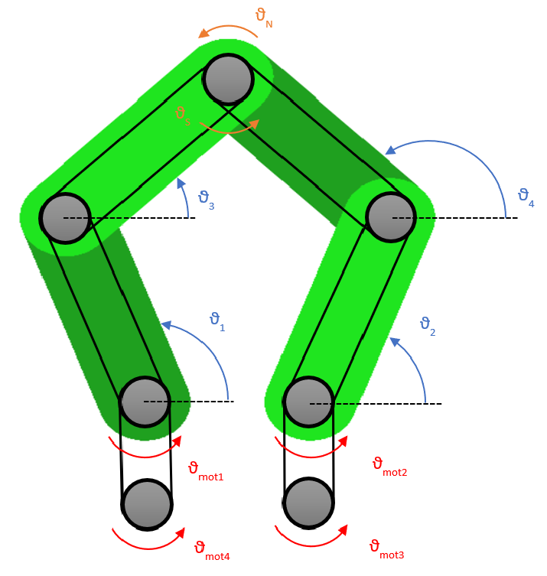
\includegraphics[scale=0.7]{Immagini/Robot1.png}
		\caption{Robot PKM}
	\end{center}
\end{figure}
\\L'obiettivo di questa tesi riguarda lo studio teorico e pratico di vari approcci di controllo, in modo da andare a trovare il migliore, in primis verrà eseguita una modellazione teorica del manipolatore, successivamente verrà svolta un'attività sperimentale che comprende l'implementazione degli schemi di controllo e la generazione di traiettorie bidimensionali e tridimensionali,
\\Escludendo l'introduzione, la tesi è articolata sette capitoli: nel secondo capitolo viene presentata l'analisi cinematica del manipolatore, in particolare verranno analizzate sia cinematica diretta che inversa, nel terzo capitolo si parla di dinamica, punti di singolarità e manipolabilità del robot; il quarto capitolo mostra la modellazione dell'\textit{end-effector}, nel nostro caso la vite; il quinto capitolo va a presentare tutte le tecnologie implementate a livello pratico, e per concludere nel sesto capitolo viene presentato il sistema reale, includendo la struttura, l'implementazione, il sistema di controllo ed i problemi riscontrati con relative soluzioni; nel settimo capitolo, infine, verranno esposte le conclusioni, grazie ad un confronto ottenuto dai risultati teorici e quelli pratici.
\subsection{Software modellazione teorica}
Per la modellazione teorica del manipolatore, abbiamo bisogno di strumenti software, in particolare utilizzeremo Matlab e Adams, il primo ci consentirà di realizzare un modello software del manipolatore, il secondo, sempre a partire da un modello ci servirà a validare i dati ottenuti dal primo in modo da verificare la loro correttezza.
\subsubsection{Matlab}
Matlab, abbreviazione di \textit{Matrix Laboratory}, è una piattaforma di calcolo ottimizzata nella risoluzione di problemi tecnici. 
Matlab è un linguaggio ad alte prestazione per la computazione tecnica, comprende: computazione, visualizzazione e programmazione in un ambiente di facile utilizzo dove i problemi e le soluzioni vengono espressi mediante una notazione matematica, gli utilizzi tipici riguardano: matematica, sviluppo di algoritmi, modellazione, simulazione, prototipazione, analisi dei dati, intelligenza artificiale, verifiche di computazione. La base di matlab è un vettore che non ha bisogno di dimensioni, in questo modo permette la risoluzione di molti problemi di computazione, specialmente quelli in formulazione vettoriale e matriciale velocemente, senza dover ricorrere all'utilizzo di linguaggi come il C. Matlab inoltre possiede delle \textit{toolbox} ovvero moduli aggiuntivi che permettono di specializzarsi in un campo, in particolare sono insieme di funzioni MATLAB che estendono l'ambiente, permettendogli di risolvere particolari classi di problemi, esempi di moduli sono reti neurali, processamento di segnali, sistemi di controllo.
\\Nel nostro caso abbiamo definito il modello teorico del robot, abbiamo poi calcolato cinematica, dinamica e punti di singolarità, nei capitoli successivi verranno mostrate le operazioni fatte. 
\subsubsection{Adams}
Adams è un software utilizzato nel campo della dinamica \textit{multibody}, in particolare nell'analisi dei modelli, infatti dopo che è stato progettato un modello può essere importato in adams ed è possibile fare analisi, simulazioni e validazioni, andando quindi a simulare la fisica del mondo reale. Adams è anche ottimizzato per problemi di grandi dimensioni.
\\Il software ha una GUI completa, infatti consente anche di disegnare direttamente il modello nello spazio tridimensionale o di importare file come STEP e IGS. I \textit{joint} possono essere aggiunti tra due corpi per vincolare il loro movimento, inoltre al sistema possono essere passati input come velocità, forze e condizioni iniziali. Adams simula il comportamento del sistema al variare del tempo, consente anche l'animazione e la computazione di proprietà come le forze, le inerzie e le accelerazioni, è anche possibile nel sistema includere elementi complessi dinamicamente come per esempio molle, corpo flessibili, contatto tra corpi.
É inoltre possibile esportare tutti i dati in formato tabellare per fare analisi successive. 
\\Per quanto riguarda il nostro caso, abbiamo utilizzato Adams per modellare il robot, assegnargli le coppie e confrontare i valori della cinematica e dinamica con quelli ottenuti da Matlab, nei capitoli successivi verrà presentato un confronto tra questi dati.
\section{Cinematica Manipolatore}
L'obiettivo di questa sezione è quello di andare ad illustrare le metodologie che ci hanno consentito di ottenere sia la cinematica diretta che quella inversa, entrambe per posizione, velocità ed accelerazione.
\par Prima di proseguire nei paragrafi seguenti andiamo a definire una tabella con i principali parametri del robot:
\begin{table}[h!]
\centering
\begin{tabular}{|c |c |c|} 
 \hline
 Nome & Descrizione  & Valore \\ [0.5ex] 
 \hline\hline
 $l [m]$ & lunghezza link  & 0.25 \\ 
 $m [kg]$ & massa link & 2.9 \\
 $c_m [m]$ & posizione centro di massa & 1.25 \\
 $J_r [kg\cdot m^2]$ & momento d'inerzia baricentrico & $5.22\cdot 10^{-2}$ \\
 $d [m]$ & lunghezza semitelaio & 0.09 \\
 \hline
\end{tabular}
\caption{Parametri manipolatore}
\label{table:1}
\end{table}
Tutti e quattro i link hanno lunghezza, massa, posizione del centro di massa e momento di inerzia uguali, per questo si è deciso di rappresentare i dati una sola volta.
\begin{figure}[ht]
\begin{center}
    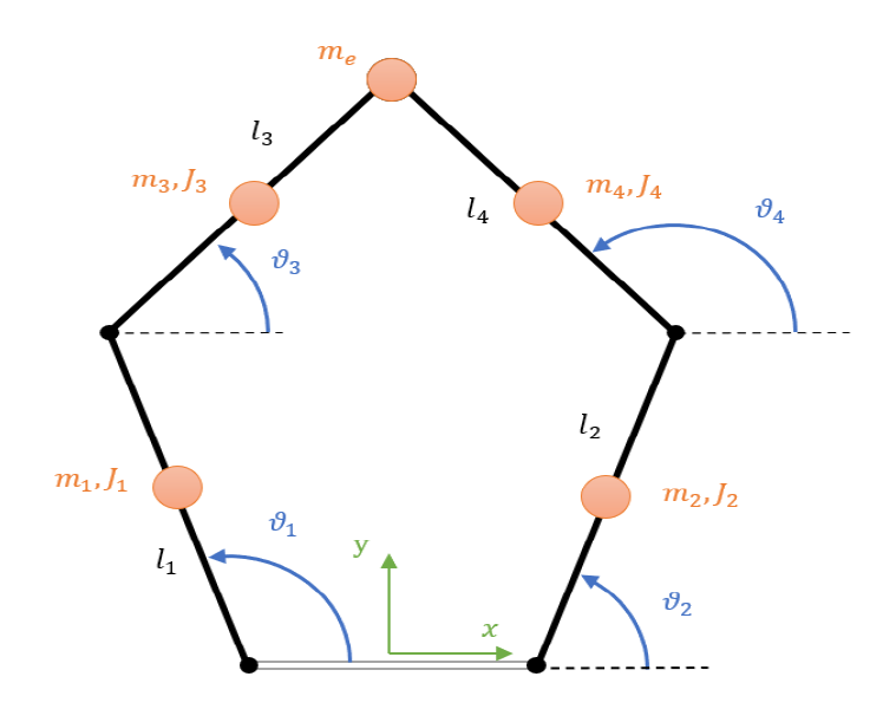
\includegraphics[scale=0.6]{Immagini/Robot2.png}
    \caption{Rappresentazione fisica del robot \label{fig:Robot1}}
\end{center}
\end{figure}
\subsection{Cinematica Diretta}
La cinematica diretta si occupa di trovare il legame tra i parametri interni del robot e la posa che esso assume, per posa si intende la posizione e l'orientamento. In questa sezione andremo ad analizzare la cinematica diretta di posizione, velocità ed accelerazione.
\subsubsection{Posizione}\label{sec:Cinematica-pos}
Nella cinematica diretta di posizione, a partire dal robot e da $\theta_1$ e $\theta_2$, riusciamo a ricavare la posizione dei link non motorizzati, i loro angoli, che sono rispettivamente $\theta_3$ e $\theta_4$ e la posizione $[x,y]$ dell'\textit{end-effector}.
L'approccio utilizzato per il calcolo della cinematica diretta è stato quello delle equazioni alle circonferenze, in particolare vengono definite due equazioni
\begin{itemize}
	\item Circonferenza centrata in E1 che passa per l'end-effector e la base del primo link
	\item Ciconferenza centrata in E2 che passa per l'end-effector e la base del secondo link
\end{itemize}
\begin{figure}[ht]
	\begin{center}
		\includegraphics[scale=0.65]{Immagini/EqCirc}
		\caption{Equazioni alle circonferenze \label{fig:eqCirc}}
	\end{center}
\end{figure}
Dalla combinazione di queste due equazioni otteniamo il seguente sistema:
\begin{equation}
    \begin{cases}
    (x-\frac{l}{2}-l\cos\theta_1)^2+(y-l\sin\theta_1)^2 = l^2 \\
    (x+\frac{l}{2}-l\cos\theta_2)^2+(y-l\sin\theta_2)^2 = l^2
    \end{cases}
\end{equation}
Da queste, andando a sviluppare i calcoli possiamo definire i parametri:
\begin{equation*}
    A = l^2 (\sin\theta_2- \sin\theta_1)^2 + (-2 d-l (\cos\theta_2 - \cos\theta_1))^2
\end{equation*}
\begin{equation*}
\begin{aligned}
   B =  -2 l^2 d (\sin\theta_2-\sin\theta_1)  (\cos(\theta_2+\theta_1) + l(\sin\theta_2-\sin\theta_1)   (-2d-l(\cos\theta_2-\cos\theta_1))\\ (-2d-2l\cos\theta_2) - 2l\sin\theta_2 (-2d-l(\cos\theta_2-\cos\theta_1))^2
\end{aligned}
\end{equation*}
\begin{equation*}
\begin{aligned}
    C = l^2 d^2 (\cos\theta_2+\cos\theta_1)^2-l d (\cos\theta_2+\cos\theta_1)(-2d-l(\cos\theta_2-\cos\theta_1) ) \\ (-2d-2l\cos\theta_2)+(d^2+2dl\cos\theta_2)(-2dl(\cos\theta_2-\cos\theta_1))^2
\end{aligned}
\end{equation*}
Il passo successivo è quello di ricavare la posizione $P=[x,y]$ dell'end-effector; si può procedere grazie alla formula risolutiva delle equazioni di secondo grado \begin{equation*}
	s_{1,2}\footnote{$\Delta = \sqrt{b^2-4ac}$} = \frac{-b \pm \Delta}{2a}
\end{equation*}
 Si può notare facilmente che la formula fornisce due risultati diversi, in una caso quando si utilizza $+\Delta$ e l'altro quando si usa $-\Delta$, è normale perché secondo il teorema fondamentale dell'algebra possono esserci fino a due soluzioni, in questo caso una coincidente con la posizione dell'end-effector e l'altra proiettata sulla base del semi-telaio. 
\begin{equation}
x = \frac{y\cdot l(\sin\theta_2 - \sin\theta_1)-l\cdot d(\cos\theta_2+\cos\theta_1)}{-2d-l(\cos\theta_2-\cos\theta_1)}, y = \frac{-B + \sqrt{B^2-4AC}}{2A} 
\end{equation}
Possiamo poi andare a trovare le posizioni dei link distali mediante relazioni geometriche nel seguente modo: 
\begin{equation*}
    E_{1X} = -d+l\cdot \cos\theta_1 \ \ \  E_{1Y}=l\cdot \sin\theta_1
\end{equation*}
e
\begin{equation*}
    E_{2X} = d+ l\cdot \cos\theta_2 \ \ \  E_{2Y} = l\cdot \sin\theta_2
\end{equation*}
Adesso che abbiamo $E_1$ ed $E_2$ possiamo andare a trovare gli angoli $\theta_3 , \theta_4$ in funzione di $\theta_1$ e $\theta_2$
\\$\theta_3 =$
\begin{equation*}
    \begin{aligned}
    2\cdot tg^{-1}\frac{\sqrt{ (\sin\theta_2 - \sin\theta_1) + \frac{1}{2}((\cos\theta_2 - \cos\theta_1 + \frac{18}{25})^2+(\frac{(\sin\theta_1-\sin\theta_2)^2}{2})^2+(\sin\theta_1-\sin\theta_2)^2)}}{(\cos\theta_2-\cos\theta_1)+\frac{(\cos\theta_2-\cos\theta_1+\frac{18}{25})^2}{2}+\frac{(\sin\theta_1-\sin\theta_2)^2}{2}+\frac{18}{25}}
    \end{aligned}
\end{equation*}
$\theta_4 =$
\begin{equation*}
    \begin{aligned}
    -2\cdot tg^{-1}\frac{\sqrt{(\sin\theta_2-\sin\theta_1)+(\frac{1}{2}(\cos\theta_2-\cos\theta_1+\frac{18}{25})^2+(\frac{(\sin\theta_1-\sin\theta_2)^2}{2})^2+(\sin\theta_1-\sin\theta_2)^2)}}
    {(\cos\theta_1 -\cos\theta_2)+\frac{(\cos\theta_2-\cos\theta_1+\frac{18}{25})^2}{2}+\frac{(\sin\theta_1-\sin\theta_2)^2}{2}+\frac{18}{25}}
    \end{aligned}
\end{equation*}
Di conseguenza, alla fine della cinematica diretta siamo riusciti ad ottenere i parametri:
\begin{equation*}
	[x,y, E1, E2, \theta_3, \theta_4]
\end{equation*}
tutti espressi in funzione di $\theta_1$ e $\theta_2$.
\subsubsection{Velocità}\label{sec:CalcoloVelCin}
Una volta ottenute le posizioni possiamo passare alle velocità, mediante la cinematica diretta di velocità possiamo ricavare le velocità sulle coordinate x e y dell'\textit{end-effector}. Possiamo infine definire una jacobiana che ci permette di trovare il rapporto appena espresso. 
\\Per semplicità di calcoli, andiamo a definire:
\begin{equation*}
    N_{21} = -l\sin\theta_1 (x+d-l\cdot \cos\theta_1 + l\cdot \cos\theta_1 (y-l\sin\theta_1))
\end{equation*}
\begin{equation*}
    N_{22} = -l\cos\theta_2\cdot \frac{y-l\sin\theta_2 (x+d-l\cos\theta_1)}{x-d-l \cos\theta_2} +l\sin\theta_2(x+d-l\cos\theta_1)
\end{equation*}
\begin{equation*}
 D_2 = \frac{y-l\sin\theta_2 (x+d-l\cos\theta_1)}{x-d-l\cos\theta_2}
\end{equation*}
Una volta definiti e calcolati questi valori possiamo andare a costruire i termini della jacobiana:  
\begin{equation*}
    J_{11} = -\frac{y-l\sin\theta_2}{x-d-l\cos\theta_2}\cdot J_{21}
\end{equation*}
\begin{equation*}
    J_{12} = -\frac{y-l\sin\theta_2}{x-d-l\cos\theta_2}\cdot J_{22} - l\sin\theta_2 + \frac{y-l\sin\theta_2}{x-d-l\cos\theta_2}\cdot l\cos\theta_2
\end{equation*}
\begin{equation*}
    J_{21} = \frac{N_{21}}{D_2}
\end{equation*}
\begin{equation*}
    J_{22} = \frac{N_{22}}{D_2}
\end{equation*}
Posizionando i termini della matrice possiamo quindi definire J come:
\begin{equation}
    J = \begin{bmatrix}
    J_{11} & J_{12} \\ J_{21} & J_{22}
    \end{bmatrix}
    \label{eq:J12}
\end{equation}
Avendo quindi definito la jacobiana possiamo ricavare la velocità dell'\textit{end-effector}  $\dot{P} = [\dot{x},\dot{y}]$, nel seguente modo:
\begin{equation}
	\begin{bmatrix}
		\dot{x} \\ \dot{y}
 	\end{bmatrix} = J \cdot \dot{\Theta} =\begin{bmatrix}
 	J_{11} & J_{12} \\ J_{21} & J_{22}
 \end{bmatrix}
 	\begin{bmatrix}
 		\dot{\theta_1} \\ \dot{\theta_2}
 	\end{bmatrix} = 
 \begin{bmatrix}
 	J_{11}\dot{\theta_1} + J_{12}\dot{\theta_2} \\
 	J_{21}\dot{\theta_1} + J_{22}\dot{\theta_2}
 \end{bmatrix}
\end{equation}
\subsubsection{Accelerazione}
Anche per quanto riguarda l'accelerazione il processo  simile a quanto visto nei paragrafi precedenti, in questo caso a partire da tutti i parametri precedentemente ricavati e da $\ddot{\Theta}$ composto da $\ddot{\theta_1}$ e $\ddot{\theta_2}$ ricaviamo le accelerazioni all'\textit{end-effector}. L'idea base è quella di risolvere la seguente equazione:
\begin{equation}
	\begin{bmatrix}
		\ddot{x} \\ \ddot{y}
	\end{bmatrix} = \dot{J}\dot{\Theta} + J\ddot{\Theta} = \dot{J}\begin{bmatrix}
	\dot{\theta_1} \\ \dot{\theta_2}
\end{bmatrix} + J \begin{bmatrix}
\ddot{\theta_1} \\ \ddot{\theta_2}
\end{bmatrix}
\end{equation}
Andando a svolgere le derivate ed i calcoli prima di poter trovare le accelerazioni definiamo: 
\begin{equation*}
\begin{aligned}
    A_{acc} = \dot{x}^2 + 2l\sin\theta_2\dot{x}\dot{\theta_2}+(l\sin\theta_2\dot{\theta_2})^2 + (x-d-l\cos\theta_2)(l\cos\theta_2\dot{\theta_2}+l\sin\theta_2\ddot{\theta_2}) +\\ \dot{y}^2-2l\cos\theta_2\dot{y}\dot{\theta_2}+(l\cos\theta_2\dot{\theta_2})^2+(y-l\sin\theta_2)(l\sin\theta_2\dot{\theta_2}^2-l\cos\theta_2\ddot{\theta_2})
    \end{aligned}
\end{equation*}
\begin{equation*}
    \begin{aligned}
    B_{acc} = \dot{x}^2+2l\sin\theta_1\dot{x}\dot{\theta_1} + (l\sin\theta_1\dot{\theta_1})^2+(x+dl\cos\theta_1)(l\cos\theta_1\dot{\theta_1}^2+l\sin\theta_1\ddot{\theta_1})+
    \\ \dot{y}^2 -2l\cos\theta_1 \dot{y}\dot{\theta_1}+(l\cos\theta_1\dot{\theta_1})^2+(y-l\sin\theta_1)(l\sin\theta_1\dot{\theta_1}^2-l\cos\theta_1\ddot{\theta_1})
    \end{aligned}
\end{equation*}
Infine, andiamo a trovare $\ddot{P} = [\ddot{x},\ddot{y}]$, nel seguente modo:
\begin{equation}
	\ddot{x} = - \frac{\ddot{y}(y-l\sin\theta_1)}{x+d-l\cos\theta_1}
\end{equation}

\begin{equation}
     \ddot{y} = \frac{\frac{B_{acc}\cdot(x-d-l\cos\theta_2)}{x+dl\cos\theta_1-A_{acc}}}{y-l\sin\theta_2-\frac{x-d-l\cos\theta_2}{(x+d-l\cos\theta_1)\cdot(y-l\sin\theta_1)}}
\end{equation}
Alla fine della cinematica diretta, a partire dai vettori delle posizioni, velocità ed accelerazioni ($\theta_1$,$\theta_2$, $\dot{\theta_1}$, $\dot{\theta_2}$, $\ddot{\theta_1}$,$\ddot{\theta_2}$) siamo riusciti ad ottenere le posizioni, velocità ed accelerazioni riferite all'\textit{end-effector}.
\subsection{Cinematica inversa}
Il problema della cinematica inversa consiste nel ricavare i valori degli angoli da assegnare ai parametri del robot per riuscire a seguire una determinata legge di moto o traiettoria a partire dalla posizione alle estremità, in questo caso l'end-effector. Anche l'analisi della cinematica inversa è stata fatta per posizione, velocità ed accelerazione.
\subsubsection{Posizione}
Nella cinematica inversa di posizione, a partire dalla posizione dell'end-effector $P = [x,y]$ andiamo a ricavare $\theta_1$ e $\theta_2$. Definiamo i seguenti parametri:
\begin{equation*}
    p = 2dl + 2xl
\end{equation*}
\begin{equation*}
	e = 2yl
\end{equation*}
\begin{equation*}
	f = x^2+d^2+y^2+2px
\end{equation*}
che serviranno per il calcolo di $\theta_1$, e:
\begin{equation*}
 a = -2dl+2xl
\end{equation*}
\begin{equation*}
	b = 2yl
\end{equation*}
\begin{equation*}
	c = x^2+d^2+y^2-2xd
\end{equation*}
che serviranno per il calcolo di $\theta_2$. 
\\Procediamo quindi con i calcoli, andando a trovare le soluzioni: 
\begin{equation}
    \theta_1 = 2\arctan\frac{e+\sqrt{p^2+e^2-f^2}}{p+f}
\end{equation}
e
\begin{equation}
    \theta_2 = 2\arctan\frac{b-\sqrt{a^2+b^2-c^2}}{a+c}
\end{equation}
Si può notare che sia per $\theta_1$ che per $\theta_2$ la somma di termini sotto la radice quadrata può dare un risultato reale o un risultato complesso, in caso che esca un risultato reale non c'è alcun problema, ma nel caso in cui $p^2 + e^2 -f^2 \le 0$ oppure $a^2 + b^2 -c^2 \le 0$ potrebbe verificarsi un caso di singolarità\footnote{I punti di singolarità sono punti nei quali il manipolatore non si comporta in modo standard, potrebbero causarsi anche rotture, verranno descritti in modo approfondito nel capitolo riguardante la dinamica}.
\subsubsection{Velocità}
Per quanto riguarda il calcolo della cinematica inversa in velocità abbiamo bisogno delle velocità $\dot{P} = [\dot{x},\dot{y}]^T$ e della Jacobiana che lega $\theta_1$ e $\theta_2$. Prendiamo l'equazione \ref{eq:J12} andiamo poi ad invertirla e ricaviamo le velocità $\dot{\theta_1}$ e $\dot{\theta_2}$ nel seguente modo:
\begin{equation}
   \begin{bmatrix} \dot{\theta_1} \\ \dot{\theta_2}  \end{bmatrix} 
    = J^{-1} \begin{bmatrix} \dot{x} \\ \dot{y} \end{bmatrix}
\end{equation}
Con
\begin{equation}
	J^{-1} = \frac{1}{J_{11}J_{22}-J_{12}J_{22}
	}\begin{bmatrix}
		J_{22} & -J_{12} \\ J_{21} & J_{11}
\end{bmatrix}
\end{equation} 
Siamo quindi riusciti ad ottenere le velocità degli angoli a partire dalle velocità all'end-effector.
\subsubsection{Accelerazione}
Anche per le accelerazioni la logica di funzionamento è la medesima, volendo trovare $\ddot{\theta_1}$ e $\ddot{\theta_2}$ a partire da $\ddot{P} = [\ddot{x},\ddot{y}]^T$ implica che dobbiamo trovare la soluzione a:
\begin{equation}
	\begin{bmatrix}
		\ddot{\theta_1} \\ \ddot{\theta_2}
	\end{bmatrix} = 
	\dot{J^{-1}}\dot{P} + J^{-1}\ddot{P} = J^{-1}(\ddot{P}-\dot{J}\dot{\Theta})
\end{equation}

\section{Dinamica Manipolatore}
Il modello dinamico del manipolatore ci fornisce una descrizione matematica della relazione che è instaurata tra le forze agenti sul robot (generalizzate) ed il movimento prodotto dalla sua struttura, cioè le configurazioni che assume nel tempo. Inizialmente, nel calcolo della dinamica sono stati usati tre metodi diversi, il metodo delle azioni vincolari, il metodo di Lagrange e quello dei lavori virtuali. Si è poi deciso di proseguire esclusivamente con il PLV. L'obiettivo di questa sezione è quello di mostrare l'approccio e i risultati ottenuti per il calcolo della dinamica diretta ed inversa.
\subsection{Prerequisiti per il calcolo della dinamica}\label{sec:prerequisiti-dinamica}
Prima di andare ad analizzare i metodi utilizzati, è importante andare a ricavare tutte le matrici delle quali avremo bisogno, in particolare è necessario andare a definire delle matrici che ci permettano di ottenere $\theta_3$ e $\theta_4$ in funzione di $\theta_1$ e $\theta_2$.
\subsubsection{Jacobiana $J_{34}$ e calcolo $\dot{\theta_3},\dot{\theta_4}$}
A partire da $\theta_1, \theta_2$ possiamo, mediante la cinematica diretta ottenere $\theta_3$ e $\theta_4$, unendo queste quattro componenti e considerando anche le velocità $\dot{\theta_1}$ e $\dot{\theta_2}$ possiamo andare a ricavare la matrice $J_{34}$ che esprime $\theta_3$ e $\theta_4$ in funzione di $\theta_1, \theta_2$ e possiamo ricavare anche $\dot{\theta_3}, \dot{\theta_4}$, per far questo andiamo a definire le seguenti quantità:
\begin{equation*}
    N_{13} = \frac{\cos\theta_4}{\sin\theta_4}\sin\theta_1-\cos\theta_1
\end{equation*}
\begin{equation*}
    N_{23} = \cos\theta_2-\frac{\cos\theta_4}{\sin\theta_4}\sin\theta_2
\end{equation*}
\begin{equation*}
    D_{13} = \cos\theta_3-\frac{\cos\theta_4}{\sin\theta_4}\sin\theta_3
\end{equation*}
Da queste tre formule possiamo andare a ricavare $\dot{\theta_3}$ nel seguente modo:
\begin{equation}
    \dot{\theta_3} = \frac{\dot{\theta_1}N_{13}}{D_{13}}+\frac{\dot{\theta_2}N_{23}}{D_{13}}
\end{equation}
Proseguiamo ora definendo le equazioni che ci serviranno per calcolare $\dot{\theta_4}$:
\begin{equation*}
    N_{14} = \frac{\sin\theta_1\cos\theta_3}{\sin\theta_3}-\frac{\cos\theta_4}{\sin\theta_4}+\frac{\cos\theta_4}{\sin\theta_4}\sin\theta_1 - \cos\theta_1
\end{equation*}
\begin{equation*}
    N_{24} = -\frac{\sin\theta_2\cos\theta_3}{\sin\theta_3}-\frac{\cos\theta_4}{\sin\theta_4}-\frac{\cos\theta_4}{\sin\theta_4}\sin\theta_2+\cos\theta_2
\end{equation*}
\begin{equation*}
    D_{14} = \frac{\sin\theta_4\cos\theta_3}{\sin\theta_3}-\frac{\cos\theta_4}{\sin\theta_4}
\end{equation*}
Otteniamo quindi:
\begin{equation}
    \dot{\theta_4} = \dot{\theta_1}\frac{N_{14}}{D_{14}}+\dot{\theta_2}\frac{N_{24}}{D_{14}}
\end{equation}
Il passo finale è quello di andare a rappresentare la matrice jacobiana che lega le velocità $\dot{\theta_3}$ e $\dot{\theta_4}$ con le velocità in ingresso al manipolatore:
\begin{equation}
    J_{34} = \begin{bmatrix}
    \frac{N_{13}}{D_{13}} & \frac{N_{23}}{D_{13}} \\
    \frac{N_{14}}{D_{14}} & \frac{N_{24}}{D_{14}}
    \end{bmatrix}
\end{equation}
%Notiamo che possiamo esprimere i parametri appena calcolati anche come:
%\begin{equation*}
%	\begin{bmatrix}
%		\dot{\theta_3} \\ \dot{\theta_4}
%	\end{bmatrix} = J_{34}\begin{bmatrix}
%	\dot{\theta_1} \\ \dot{\theta_2}
%\end{bmatrix}
%\end{equation*}
\subsubsection{Jacobiana $\dot{J_{34}}$ e calcolo di $\ddot{\theta_3}, \ddot{\theta_4}$}
Per andar ad ottenere la jacobiana finale, ed i valori delle accelerazioni sui link distali occorre derivare tutti gli elementi visti in precedenza, in particolare:
\begin{equation*} %  N11p =  N13p
    \dot{N_{13}} = \frac{-1}{\sin^2\theta_4\cdot\dot{\theta_4}\sin\theta_1}+\frac{\cos\theta_4}{\sin\theta_4}\cos\theta_1\dot{\theta_1}+\sin\theta_1\dot{\theta_1}
\end{equation*}
\begin{equation*} %N12p = N23p
   \dot{N_{23}} =\frac{1}{\sin^2\theta_4\cdot\dot{\theta_4}\sin\theta_2}-\frac{\cos\theta_4}{\sin\theta_4}\cos\theta_2\dot{\theta_2}-\sin\theta_2\dot{\theta_2}
\end{equation*}
\begin{equation*} % D1p = D13p
  \dot{D_{13}} =  -\sin\theta_3\dot{\theta_3} + \frac{1}{\sin^2\theta_4}\dot{\theta_4}\sin\theta_3 -\frac{ \cos\theta_4} {\sin\theta_4}\cos\theta_3\dot{\theta_3}
\end{equation*}
\begin{equation*} % N21p = N14p
\begin{aligned}
    \dot{N_{14}} = \cos\theta_1\dot{\theta_1}\bigg(\frac{\cos\theta_3}{\sin\theta_3}-\frac{\cos\theta_4}{\sin\theta_4}\bigg) + \sin\theta_1\bigg(\frac{1}{\sin^2\theta_3}\dot{\theta_3}+\frac{1}{\sin^2\theta_4}\dot{\theta_4}\bigg)+\\+\frac{-1}{\sin^2\theta_4}\dot{\theta_4}\sin\theta_1 +\cot\theta_4\cos\theta_1\dot{\theta_1}+\sin\theta_1\dot{\theta_1}
    \end{aligned}
\end{equation*}
\begin{equation*} % N22p = N24p
    \begin{aligned}
    \dot{N_{24}} = -\cos\theta_2\dot{\theta_2}\bigg(\frac{\cos\theta_3}{\sin\theta_3} - \frac{\cos\theta_4}{\sin\theta_4} \bigg) - \sin\theta_2\bigg(\frac{-1}{\sin^2\theta_3}\dot{\theta_3} + \frac{1}{\sin^2\theta_4}\dot{\theta_4}\bigg) -\\
    - \frac{-1}{\sin^2\theta_4}\dot{\theta_4}\sin\theta_2-\cot\theta_4\cos\theta_2\dot{\theta_2}-\sin\theta_2\dot{\theta_2}
    \end{aligned}
\end{equation*}
\begin{equation*} % D2p = D14p
   \dot{D_{14}} = \cos\theta_4\dot{\theta_4}(\cot\theta_3-\cot\theta_4)+\sin\theta_4\bigg(\frac{-1}{\sin^2\theta_3}\dot{\theta_3} + \frac{1}{\sin^2\theta_4}\dot{\theta_4}\bigg)
\end{equation*}
Esprimendo la matrice jacobiana $\dot{J_{34}}$ in funzione dei parametri appena trovati scriviamo:
\begin{equation}
    \dot{J_{34}} =
    \begin{bmatrix}
    \frac{\dot{N_{13}}D_{13}-N_{13}\dot{D_{13}}}{D_{13}^2} & 
     \frac{\dot{N_{23}}D_{13}-N_{23}\dot{D_{13}}}{D_{13}^2} \\
    \frac{\dot{N_{14}}D_{14}-N_{14}\dot{D_{14}}}{D_{14}^2} &
     \frac{\dot{N_{24}}D_{14}-N_{24}\dot{D_{14}}}{D_{14}^2}
    \end{bmatrix}
\end{equation}
Per concludere andiamo a trovare:
\begin{equation}
    \begin{bmatrix}
    \ddot{\theta_3} \\ \ddot{\theta_4}
    \end{bmatrix}
    = 
    \dot{J_{34}}\begin{bmatrix}
    \dot{\theta_1} \\ \dot{\theta_2}
    \end{bmatrix} + 
    J_{34} \begin{bmatrix}
    \ddot{\theta_1} \\ \ddot{\theta_2}
    \end{bmatrix}
\end{equation}
\subsubsection{Matrici di inerzia}
Per trovare la soluzione all'equazione del PLV introduciamo le matrici che hanno avuto un ruolo fondamentale nel calcolo:
\begin{equation*}
    J_1 = \begin{bmatrix}
     -0.5l\sin\theta_1 & 0 \\ 0.5l\cos\theta_1 & 0
    \end{bmatrix} \Rightarrow
    \dot{J_1} = \begin{bmatrix}
     -0.5l\cos\theta_1\dot{\theta_1} & 0 \\ -0.5l\sin\theta_1\dot{\theta_1} & 0
    \end{bmatrix}
\end{equation*}
\begin{equation*}
    J_2 = \begin{bmatrix}
           0 & -0.5*l*\sin\theta_2 \\
           0 & 0.5*l*\cos\theta_2 
           \end{bmatrix}
           \Rightarrow
   \dot{J_2} = \begin{bmatrix} 0 & -0.5l\cos\theta_2\dot{\theta_2} \\
           0 & -0.5l\sin\theta_2\dot{\theta_2}
           \end{bmatrix}
\end{equation*}
\begin{equation*}
    J_3 = \begin{bmatrix}
    -l\sin\theta_1+0.5\sin\theta_3\cdot J_{34}(1,1) & 
    -0.5l\sin\theta_3\cdot J_{34}(1,2) \\
    l\cos\theta_1+0.5\cos\theta_3\cdot J_{34}(1,1) & 
    0.5l\cos\theta_3\cdot J_{34}(1,2)
    \end{bmatrix}
\end{equation*}
\begin{equation*}
    J_4 = \begin{bmatrix}
    -0.5l\sin\theta_4\cdot J_{34}(2,1) &
    -l\sin\theta_2+0.5\sin\theta_4\cdot J_{34}(2,2) \\
    0.5l\cos\theta_4\cdot J_{34}(2,1) &
    l\cos\theta_2+0.5\cos\theta_4\cdot J_{34}(2,2)
    \end{bmatrix}
\end{equation*}
\begin{equation*}
    J_E = \begin{bmatrix}
    -l(\sin\theta_1+\sin\theta_3\cdot J_{34}(1,1)) & 
    -l\sin\theta_3 \cdot J_{34}(1,2) \\
    l(\cos\theta_1+\cos\theta_3\cdot J_{34}(1,1)) &
    l\cos\theta_3 \cdot J_{34}(1,2)
    \end{bmatrix}
\end{equation*} 
Importanti nel calcolo della dinamica saranno anche le derivate delle matrici che abbiamo appena visto, ovvero $\dot{J_3}, \dot{J_4}, \dot{J_E}$. 
\subsection{Principio dei lavori virtuali}
Il lavoro virtuale è il lavoro svolto da una forza reale che agisce attraverso uno spostamento virtuale o da una forza virtuale che agisce attraverso uno spostamento reale.
Uno spostamento virtuale è uno spostamento coerente con i vincoli della struttura, cioè che soddisfano le condizioni al contorno in corrispondenza degli appoggi.
Una forza virtuale è un qualsiasi sistema di forze in equilibrio.
Per problemi nei quali i corpo sono composti da membri interconnessi che si possono muovere relativamente gli uni rispetto agli altri, originando diverse configurazioni di equilibrio un buon metodo di analisi è quello del "principio dei lavori virtuali" conosciuto anche come PLV ci permette di ottenere una relazione relativamente semplice, è basato sul concetto di Lavoro sviluppato da una forza, ed inoltre ci consente di analizzare la stabilità di un sistema in equilibrio.
\begin{equation}
    \sum_{i=1}^m F_j\delta q_j\label{eq:din}
\end{equation}
\subsection{Dinamica inversa}
Il problema della dinamica inversa consiste nel determinare le coppie ai giunti necessarie per generare il movimento a partire da posizione, velocità ed accelerazione.
\\Andando a sviluppare l'equazione dei principi virtuali troviamo le coppie dei link motorizzati nel seguente modo:
\begin{equation*}
\begin{aligned}
    \delta \theta^T C = \delta \theta^T I_2 \ddot{\theta} + \delta \theta^T J_{34}^T I_2(J_{34}\ddot{\theta}+\dot{J_{34}}\dot{\theta})+ \delta \theta^T \frac{25}{4}ml^2\\\bigg(\begin{bmatrix}
    -\cos\theta_1 & -\sin\theta_1 \\ -\cos\theta_2 & -\sin\theta_2
    \end{bmatrix}
    \dot{\theta^2} + \begin{bmatrix}
    -\sin\theta_1 & \cos\theta_1 \\ -\sin\theta_2 & \cos\theta_2
    \end{bmatrix} \ddot{\theta}\bigg) +  \delta \theta^T J_{34}^T\frac{9}{4}l^2(m+m_v)\\\bigg(\begin{bmatrix}
    -\cos\theta_3 & -\sin\theta_3 \\ -\cos\theta_4 & -\sin\theta_4
    \end{bmatrix}J_{34}J_{34}^T\dot{\theta^2}+\begin{bmatrix}
    -\sin\theta_3 & \cos\theta_3 \\ -\sin\theta_4 & \cos\theta_4
    \end{bmatrix}(\dot{J_{34}}\dot{\theta}+J_{34}\ddot{\theta})\bigg)
    \end{aligned}
\end{equation*}
Semplificando e raccogliendo possiamo esprimere l'equazione come:
\begin{equation}
    \tau = M \ddot{\theta} + K \dot{\theta}
    \label{eq:dinamicaInv}
\end{equation}
Dove:
\begin{equation}
    M = J_r I_2 + m(J_1^T J_1 + J_2^TJ_2+J_3^TJ_3+J_4^TJ_4)+J_rJ_{34}^TJ_{34} + m_vJ_E^TJ_E
    \label{eq:M}
\end{equation}
\begin{equation}
    K = m(J_1^T\dot{J_1}+J_2^T\dot{J_2}+J_3^T\dot{J_3}+J_4^T\dot{J_4})+J_rJ_{34}^T\dot{J_{34}}+m_vJ_E^T\dot{J_E}
    \label{eq:K}
\end{equation}
Sostituendo, possiamo andare ad esprimere l'equazione \ref{eq:dinamicaInv} nel seguente modo:
\begin{equation}
    \begin{bmatrix}
    \tau_1 \\ \tau_2
    \end{bmatrix} = 
    M\begin{bmatrix}
    \ddot{\theta_1} \\ \ddot{\theta_2}
    \end{bmatrix}
    + K \begin{bmatrix}
    \dot{\theta_1} \\ \dot{\theta_2}
    \end{bmatrix}
\end{equation}
% CONTROLLA
Per tutti i calcoli svolti fino ad adesso le coppie devono considerarsi prese all'end-effector
\subsection{Dinamica diretta}
Il problema della dinamica diretta invece consiste nel determinare le accelerazioni ai giunti a partire dalle coppie, dalla posizione e velocità iniziali di entrambi i link.
\\Identifichiamo quindi $\Theta$ come vettore delle condizioni iniziali, in particolare possiamo definirlo come segue:
\begin{equation*}
    \Theta = \begin{bmatrix}
    \theta_1(t_0) \\ \theta_2(t_0) \\ \dot{\theta_1(t_0)} \\ \dot{\theta_2(t_0)}
    \end{bmatrix}
\end{equation*}
Possiamo andare a calcolare $\theta_3$ e $\theta_4$ come abbiamo visto in precedenza nella sezione \ref{sec:Cinematica-pos}, e di conseguenza anche tutte le matrici viste nella sezione \ref{sec:prerequisiti-dinamica}. Con tutti questi dati possiamo andare a ricalcolare le equazioni \ref{eq:M} e \ref{eq:K}. 
\\Andiamo ora a definire l'equazione della dinamica diretta andando ad invertire l'equazione \ref{eq:dinamicaInv} in questo modo:
\begin{equation}
    \ddot{\theta} = M^{-1}(-K\dot{\theta}+\tau)
    \label{eq:dinamicaDiretta}
\end{equation}
Infine, da questa possiamo andare anche a calcolare velocità e posizioni integrando l'equazione.
\\Avendo sia il grafico della legge di moto iniziale relativa a posizione, velocità ed accelerazione assegnata agli angoli $\theta_1$ e $\theta_2$, che le coppie, possiamo andare a calcolare la dinamica con le coppie e le condizioni iniziali e \textit{plottare} il confronto tra queste due curve. In particolare andiamo a vedere il confronto su accelerazioni, velocità e posizioni sia per $\theta_1$ che per $\theta_2$: 
\begin{figure}[!ht]
\begin{subfigure}{.45\textwidth}
  \centering
  % include first image
  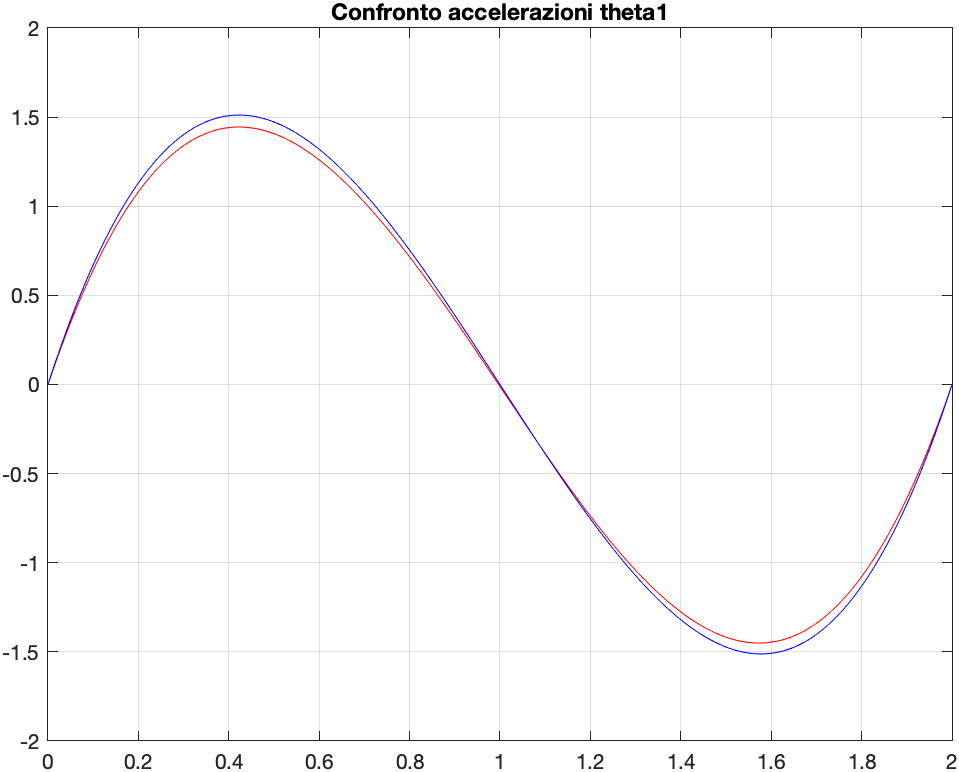
\includegraphics[width=.78\linewidth]{Immagini/Dinamica/confracct1.png}  
  \caption{Accelerazione $\theta_1$}
  \label{fig:sub-first}
\end{subfigure}
\begin{subfigure}{.45\textwidth}
  \centering
  % include second image
  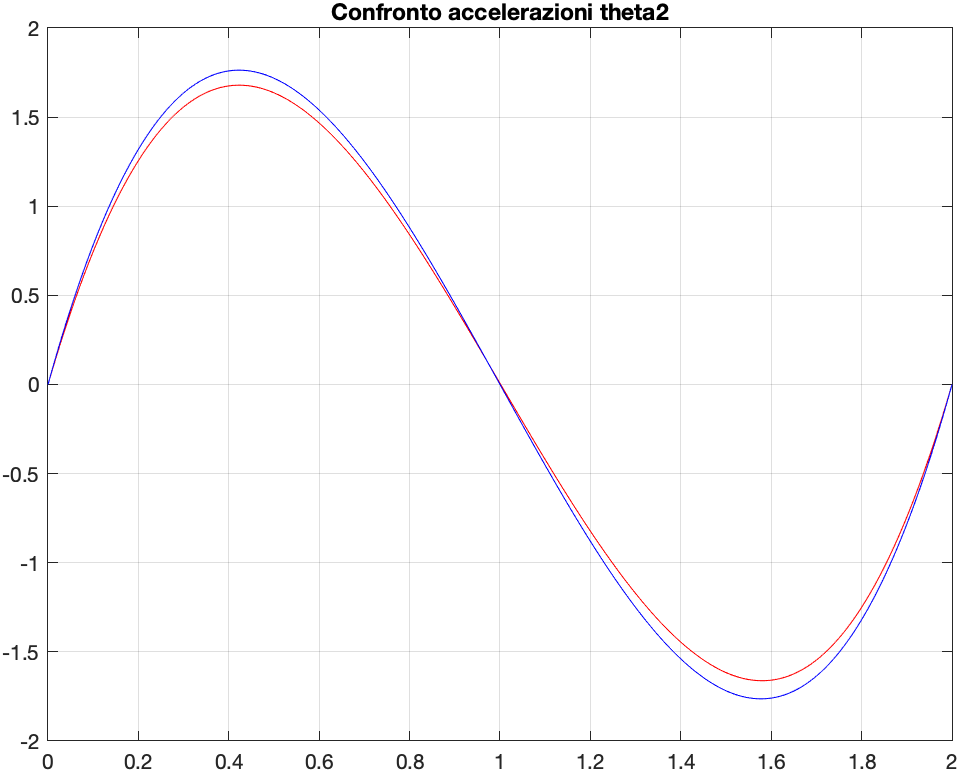
\includegraphics[width=.78\linewidth]{Immagini/Dinamica/confracct2.png}  
  \caption{Accelerazione $\theta_2$}
  \label{fig:sub-second}
\end{subfigure}
\caption{Confronto dinamica leggi di moto su accelerazioni}
\end{figure}
\begin{figure}[!ht]
\begin{subfigure}{.45\textwidth}
  \centering
  % include first image
  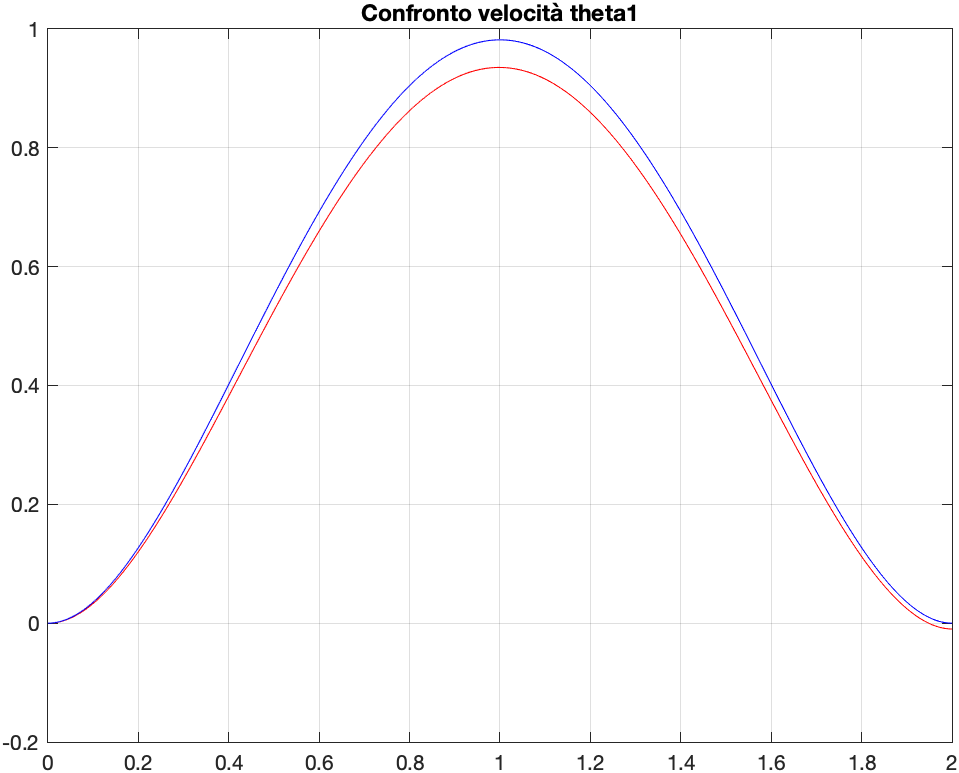
\includegraphics[width=.78\linewidth]{Immagini/Dinamica/confrvelt1.png}  
  \caption{Velocità $\theta_1$}
  \label{fig:sub-firstv}
\end{subfigure}
\begin{subfigure}{.45\textwidth}
  \centering
  % include second image
  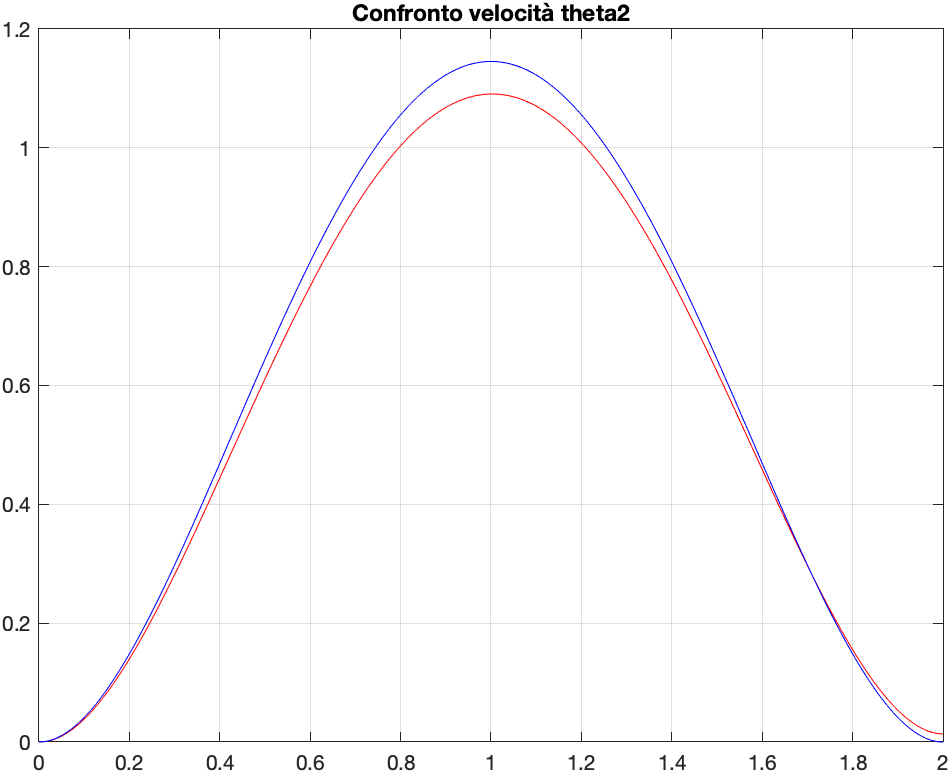
\includegraphics[width=.78\linewidth]{Immagini/Dinamica/confrtvelt2.png}  
  \caption{Velocità $\theta_2$}
  \label{fig:sub-secondv}
\end{subfigure}
\caption{Confronto dinamica leggi di moto su velocità}
\end{figure}
\begin{figure}[!ht]
\begin{subfigure}{.45\textwidth}
  \centering
  % include first image
  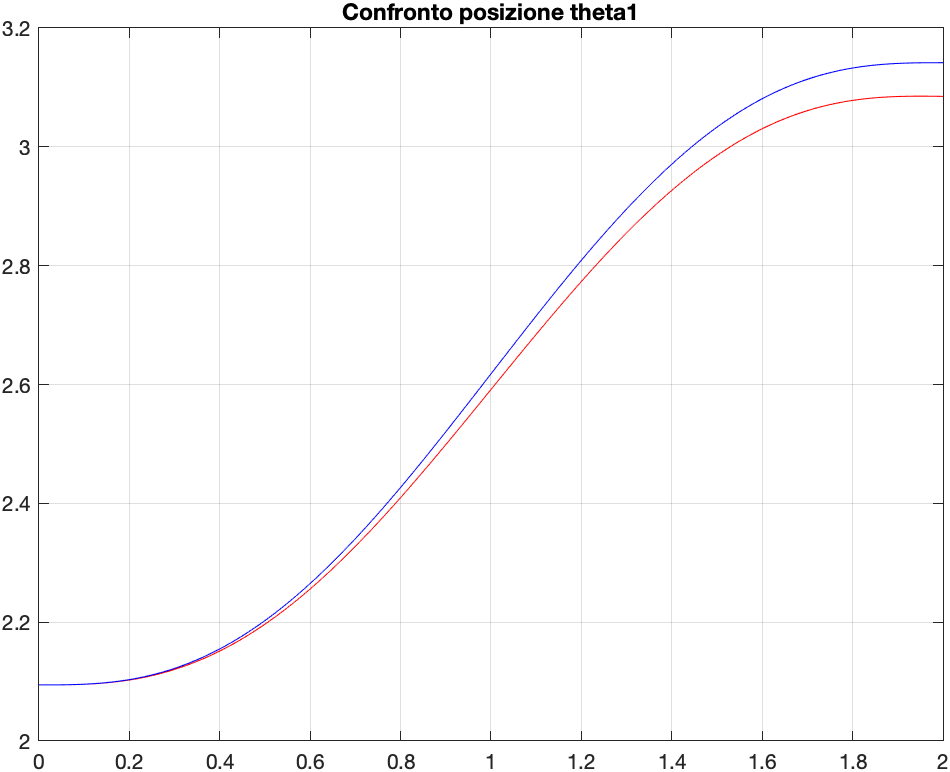
\includegraphics[width=.78\linewidth]{Immagini/Dinamica/confrpost1.png}  
  \caption{Posizione $\theta_1$}
  \label{fig:sub-firsta}
\end{subfigure}
\begin{subfigure}{.45\textwidth}
  \centering
  % include second image
  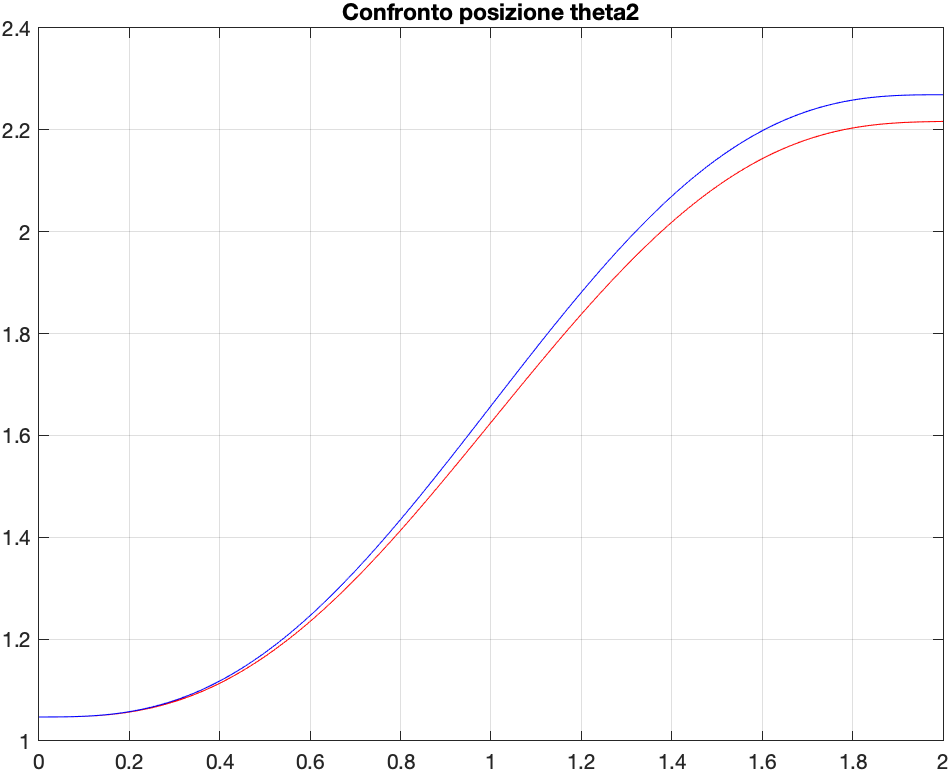
\includegraphics[width=.78\linewidth]{Immagini/Dinamica/confrpost2.png}  
  \caption{Posizione $\theta_2$}
  \label{fig:sub-seconda}
\end{subfigure}
\caption{Confronto dinamica leggi di moto su posizioni}
\end{figure}
Una volta calcolati tutti i parametri di nostro interesse andiamo a costruire il modello simulink che sarà utile per una visione d'insieme:
\begin{figure}[ht]
	\begin{center}
		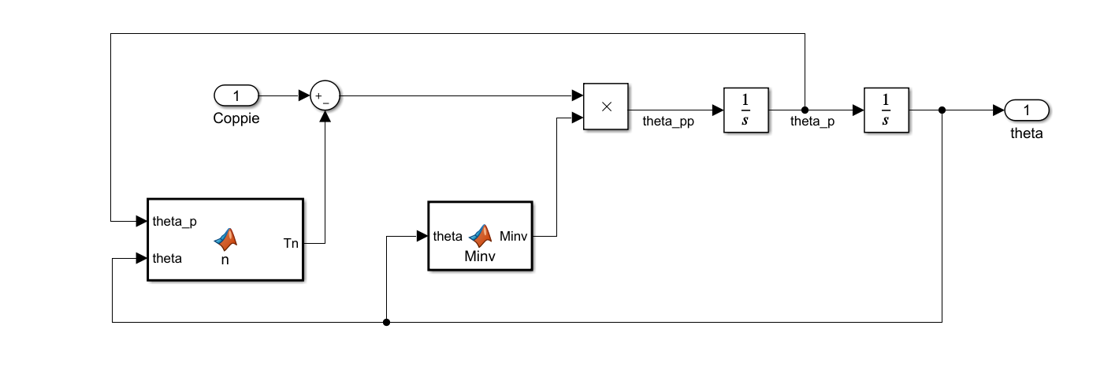
\includegraphics[scale=0.55]{Immagini/Dinamica/ModSimulink}
		\caption{Modello simulink manipolatore}
	\end{center}
\end{figure}
\subsubsection*{Modellazione su Adams}
\addcontentsline{toc}{subsubsection}{Modellazione su Adams}
Per quanto riguarda la modellazione su adams, è stato realizzato un prototipo del manipolatore composto da aste rigide, i due link motorizzati sono fissati mediante delle cerniere ed abbiamo anche la presenza dell'end-effector.
\begin{figure}[!ht]
	\begin{subfigure}{.5\textwidth}
		\centering
		% include first image
		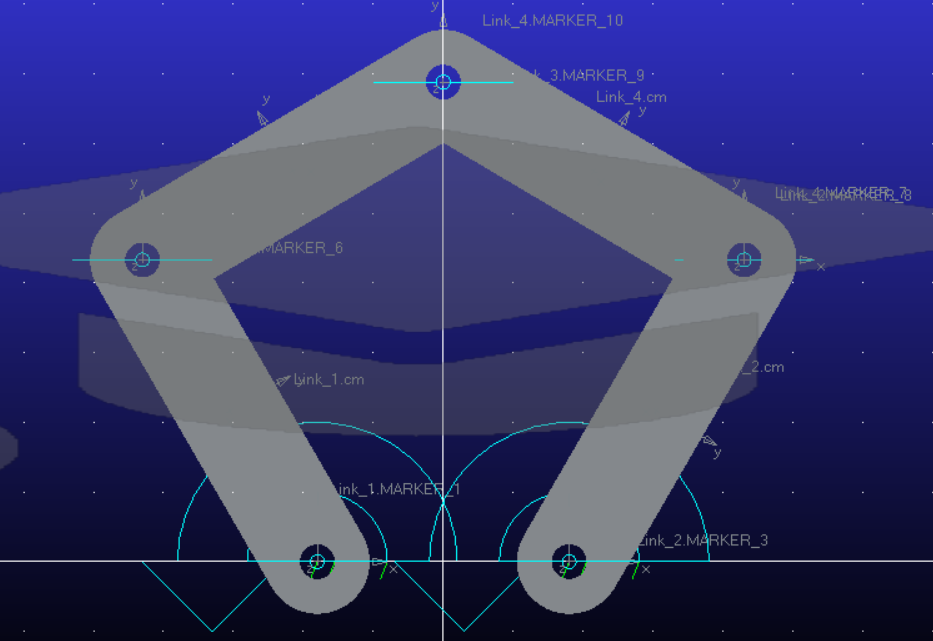
\includegraphics[width=.9\linewidth]{Immagini/Dinamica/adams1.png}  
		\caption{Vista dall'alto}
		\label{fig:sub-adams1}
	\end{subfigure}
	\begin{subfigure}{.5\textwidth}
		\centering
		% include second image
		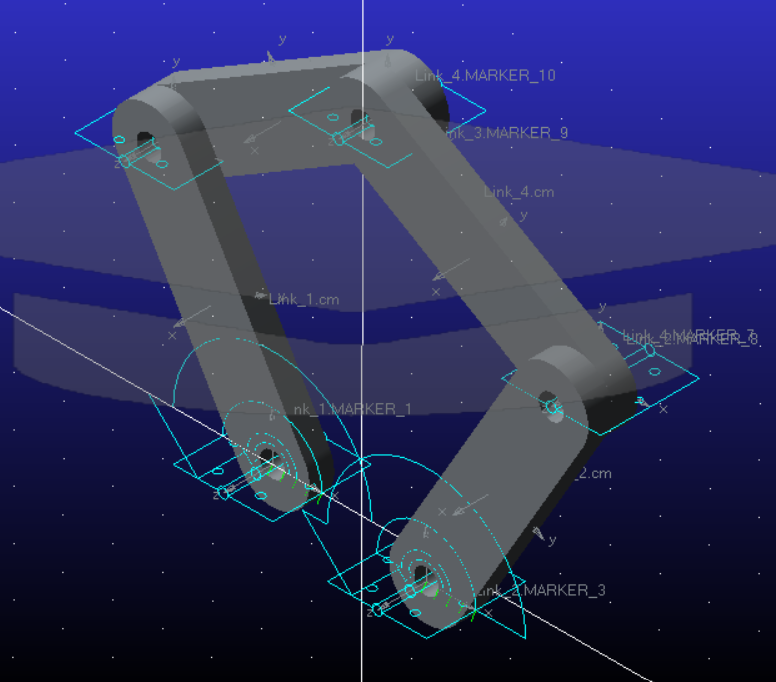
\includegraphics[width=.8\linewidth]{Immagini/Dinamica/adams2.png}  
		\caption{Vista in diagonale}
		\label{fig:sub-adams2}
	\end{subfigure}
	\caption{Modello Adams manipolatore 5R}
\end{figure}
Una volta definiti i vincoli e le modalità di movimento del manipolatore si è passati alla fase successiva ovvero quella dell'analisi del modello e della simulazione, andando ad assegnare leggi di moto al modello adams e verificare il suo comportamento rispetto al modello creato su simulink.
\subsubsection*{Validazione e confronto}
\addcontentsline{toc}{subsubsection}{Validazione e confronto}
Le leggi di moto assegnate al modello adams sono state anche assegnate nella stessa maniera al modello simulink, in particolare sono state utilizzate: 
\begin{table}[h!]
	\centering
	\begin{tabular}{|c|c|} 
		\hline
		Motore & Legge di moto  \\
		\hline\hline
		Motore 1 ($\theta_1$)& Sinusoidale $sin$ \\
		Motore 2 ($\theta_2$)& Sinusoidale $2\sin$ \\
		\hline
	\end{tabular}
	\caption{Leggi di moto validazione}
	\label{table:ldmAdams}
\end{table}
Una volta assegnata la legge ed eseguita la simulazione si è fatto un confronto:
\begin{figure}[!ht]
	\begin{subfigure}{.5\textwidth}
		\centering
		% include first image
		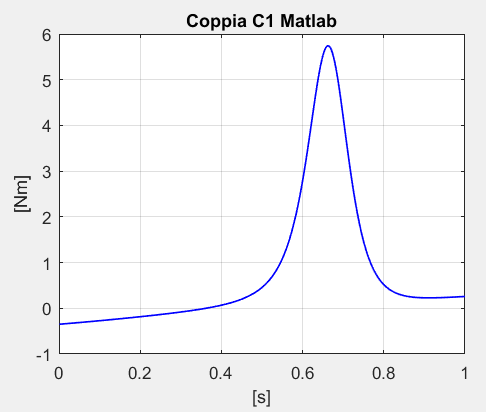
\includegraphics[width=.9\linewidth]{Immagini/Dinamica/c1matlab.png}  
		\caption{Coppia C1 Matlab}
		\label{fig:leggiC1M}
	\end{subfigure}
	\begin{subfigure}{.5\textwidth}
		\centering
		% include second image
		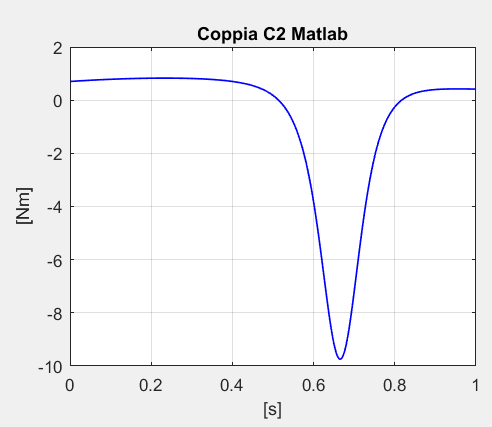
\includegraphics[width=.9\linewidth]{Immagini/Dinamica/c2matlab.png}  
		\caption{Coppia C2 Matlab}
		\label{fig:leggiC2M}
	\end{subfigure}
	\caption{Coppie in uscita Simulink}
\end{figure}
\begin{figure}[!ht]
	\begin{subfigure}{.5\textwidth}
		\centering
		% include first image
		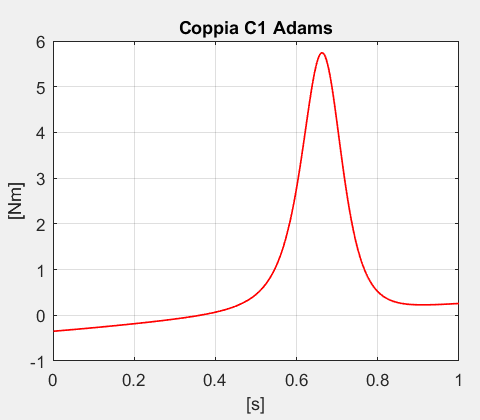
\includegraphics[width=.9\linewidth]{Immagini/Dinamica/c1adams.png}  
		\caption{Coppia C1 Adams}
		\label{fig:leggiC1A}
	\end{subfigure}
	\begin{subfigure}{.5\textwidth}
		\centering
		% include second image
		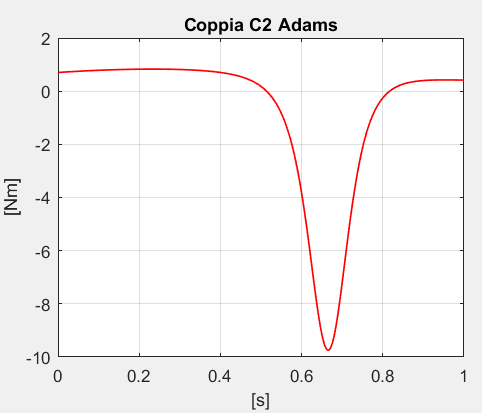
\includegraphics[width=.9\linewidth]{Immagini/Dinamica/c2adams.png}  
		\caption{Coppia C2 Adams}
		\label{fig:leggiC2A}
	\end{subfigure}
	\caption{Coppie in uscita Adams}
\end{figure}
Andando poi a fare una differenza tra questi due grafici riusciamo a trovare l'andamento dell'errore sulle coppie:
\begin{figure}[!ht]
	\begin{subfigure}{.5\textwidth}
		\centering
		% include first image
		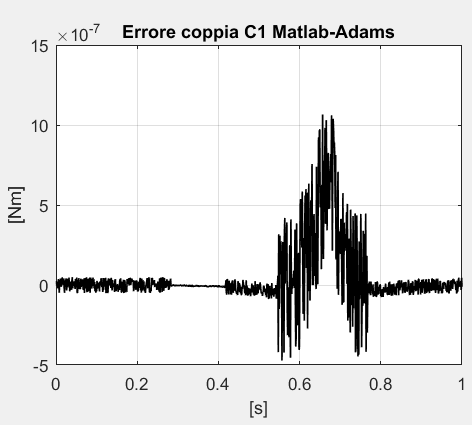
\includegraphics[width=.9\linewidth]{Immagini/Dinamica/confrc1.png}  
		\caption{Errore coppia C1}
		\label{fig:errC1}
	\end{subfigure}
	\begin{subfigure}{.5\textwidth}
		\centering
		% include second image
		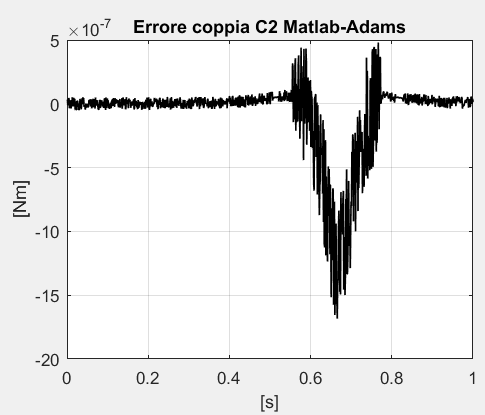
\includegraphics[width=.9\linewidth]{Immagini/Dinamica/confrc2.png}  
		\caption{Errore coppia C2}
		\label{fig:errC2}
	\end{subfigure}
	\caption{Errore Simulink-Adams}
\end{figure}
Analizzando il grafico vediamo che l'errore è nell'ordine di $10^{-7}$ di conseguenza è possibile vedere che la validazione ha portato un risultato positivo in quanto le coppie del modello Simulink e le coppie del modello Adams sono praticamente identiche a parte un fattore d'errore dato dalle diverse modalità di calcolo/integrazione.
\subsection{Punti di singolarità}
Nell'ambito matematico, una singolarità è un punto nel quale un oggetto non è definito, oppure un punto nel quale l'oggetto non ha un comportamento normale, nel nostro caso i punti di singolarità saranno punti che andranno a delimitare lo spazio di lavoro del robot. Definiamo spazio di lavoro del robot tutto un insieme di punti nei quali il robot ha un funzionamento normale e non presenta problematiche.\footnote{Passando per un punto di singolarità il robot potrebbe aver problemi che potrebbero causare anche la rottura di parti meccaniche} Andando a considerare la foto vista nell'introduzione, possiamo trovare sei casi di punti di singolarità, in particolare però non sono punti ma sono traiettorie. Di conseguenza il robot avrà come spazio di lavoro, tutto lo spazio che è interno (delimitato) da queste traiettorie.
\subsubsection*{Primo e secondo caso}
\addcontentsline{toc}{subsubsection}{Primo e secondo caso}
In questo primo caso abbiamo $\overrightarrow{CD}$ che è parallelo a $\overrightarrow{DE}$, schematicamente possiamo andarlo a rappresentare nel seguente modo
\begin{figure}[ht]
	\begin{center}
		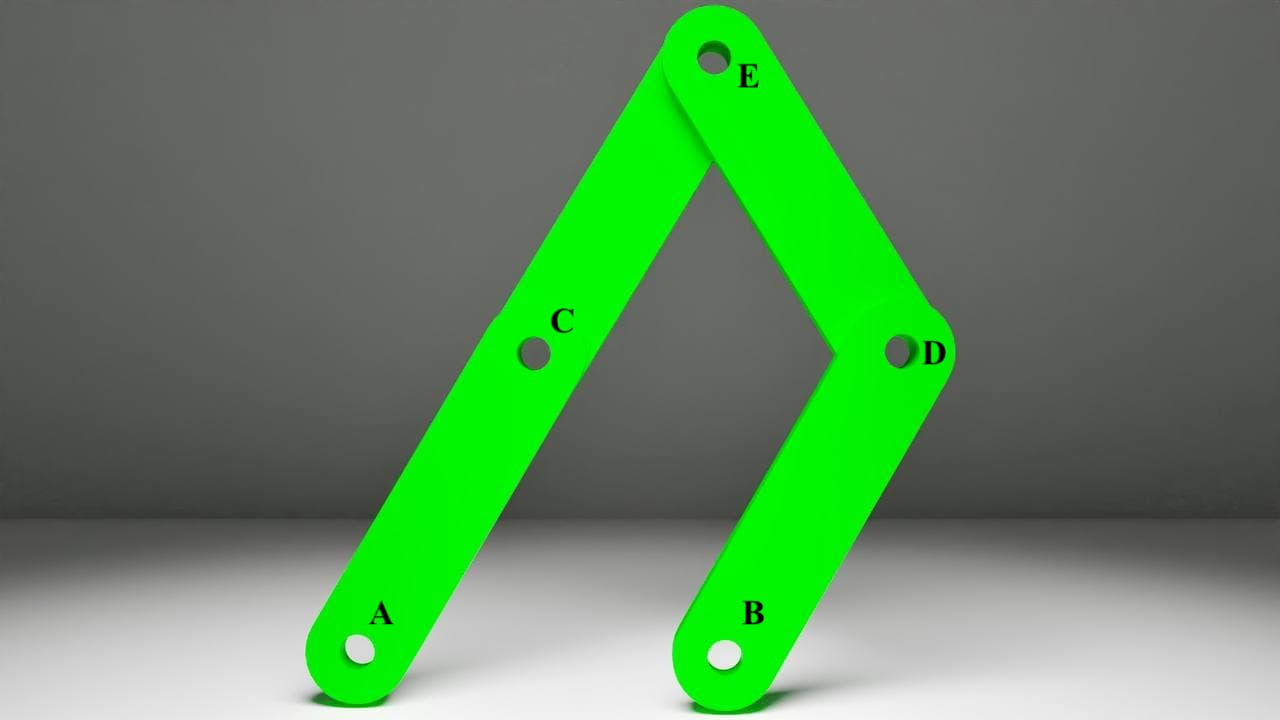
\includegraphics[scale=0.4]{Immagini/Singolarity/1}
		\caption{Caso 1 singolarità}
	\end{center}
\end{figure}
\\Lasciando la x libera possiamo ricavare la y come:
\begin{equation}
    y_1 = \sqrt{4l^2-(x-d)^2}
\end{equation}
Per quanto riguarda il secondo caso è molto simile al primo, la differenza sta nel fatto che abbiamo la catena $\overrightarrow{AB}$ parallela a $\overrightarrow{BC}$ 
\begin{figure}[ht]
	\begin{center}
		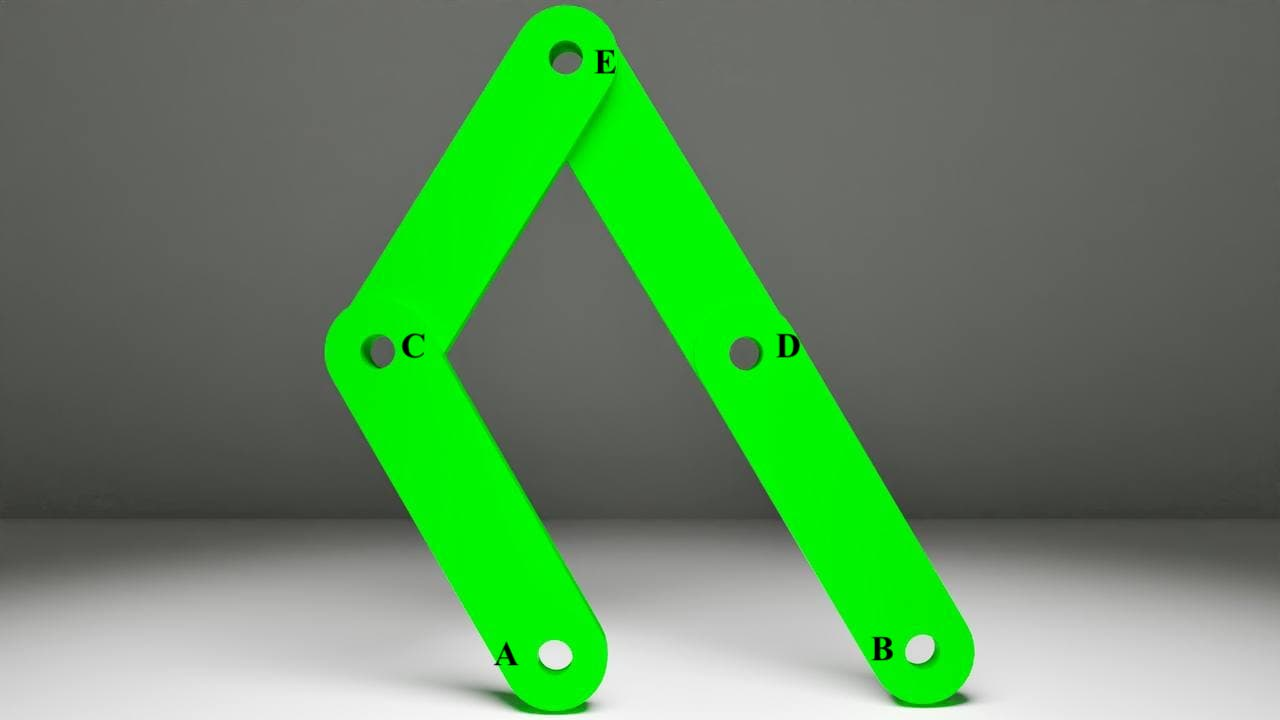
\includegraphics[scale=0.4]{Immagini/Singolarity/2}
		\caption{Caso 2 singolarità}
	\end{center}
\end{figure}
Il procedimento è simile a prima, lasciando sempre la x libera possiamo trovare la y come:
\begin{equation}
    y_2 = \sqrt{4l^2-(x+d)^2}
\end{equation}
Entrambi i casi producono come risultato una circonferenza.
\subsubsection*{Terzo caso}
\addcontentsline{toc}{subsubsection}{Terzo caso}
Il terzo caso di singolarità avviene quando i due link non motorizzati sono paralleli, questa configurazione aggiunge un grado di libertà al sistema, in quanto l'end-effector per muoversi ha necessità di una maggior coppia per riuscire a superare la situazione di stallo
\begin{figure}[ht]
	\begin{center}
		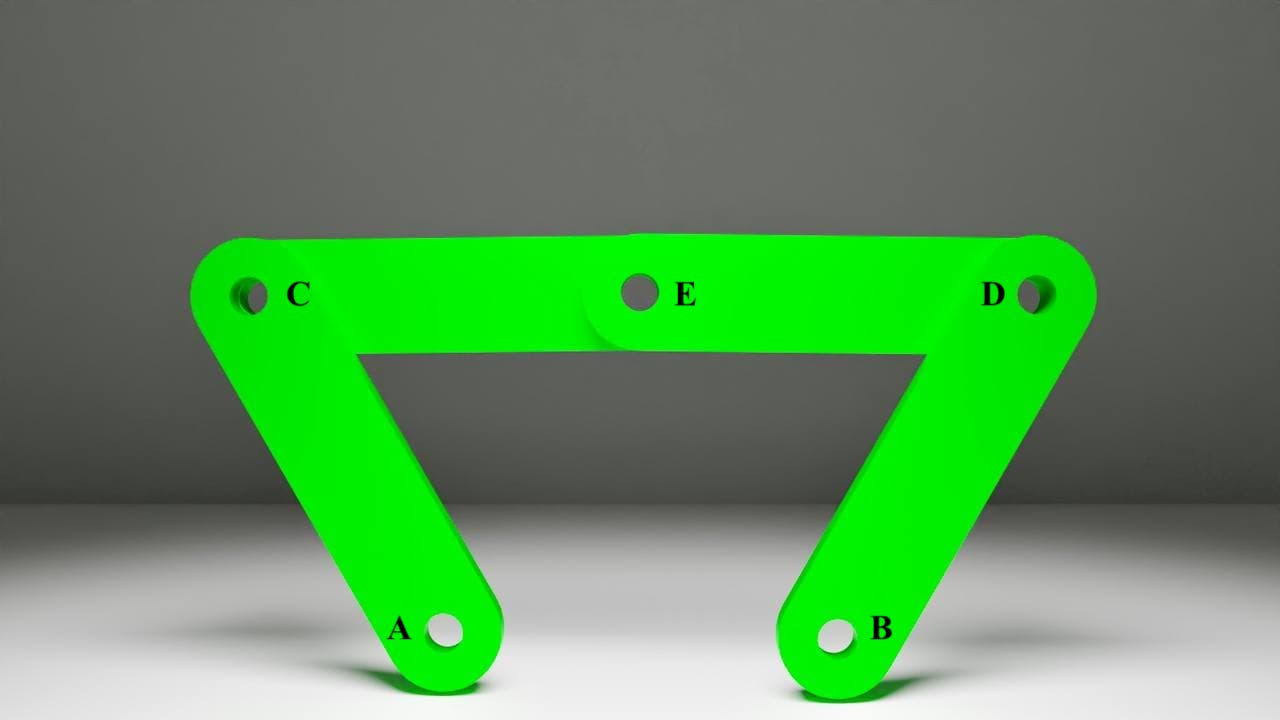
\includegraphics[scale=0.4]{Immagini/Singolarity/5}
		\caption{Caso 3 singolarità}
	\end{center}
\end{figure}
\\Per quanto riguarda la soluzione, andiamo a considerare $\theta_1$ che varia da 0 a $360^\circ$ e andiamo a cercare le coppie di valori $[x,y]$ relative alla singolarità. Uscirà un'equazione di secondo grado, con i seguenti coefficienti:
\begin{equation*}
	a = l^2\sin^2\theta_1 + 4d^2-4dl\cos\theta_1 + l^2\cos^2\theta_1
\end{equation*}
\begin{equation*}
	b = 2l^3\sin\theta_1 + 2dl^2\sin\theta_1\cos\theta_1-2dl\sin\theta_1(2d-2l\cos\theta_1)
\end{equation*}
\begin{equation*}
	c = l^2(l^2+d^2\cos^2\theta_1+2ld\cos\theta_1)-2dl(l+d\cos\theta_1)(2d-l\cos\theta_1)+d^2-l^2(2d-l\cos\theta_1)^2
\end{equation*}
Risolviamo l'equazione di secondo grado:
\begin{equation*}
	\Delta = b^2-4ac
\end{equation*}
Andiamo a trovare le radici y di quest'equazione, definendo poi: $sx = -b+l\cos\theta_1$ ed $sy = l\sin\theta_1$ possiamo andare a trovare le soluzioni dell'equazione come:
\begin{equation}
	x_3 = \bigg|\frac{x_{3p}+sx}{2}\bigg|, y_3 = \bigg|\frac{y_{3p}+sy}{2}\bigg|
\end{equation}
Con 
\begin{equation*}
	x_{3p} = \frac{l^2+y_{3p}l\sin\theta_1+ld\cos\theta_1}{2d-l\cos\theta_1}
\end{equation*}
\subsubsection*{Quarto e quinto caso}
\addcontentsline{toc}{subsubsection}{Terzo e quarto caso}
Il quarto e quinto caso sono casi di singolarità non realizzabili nella pratica, ma sono di interesse teorico. Il primo caso prevede che la posizione dell'end-effector coincida con la posizione del primo giunto motorizzato e nell'altro caso coinciderà con il secondo giunto motorizzato. Come soluzioni avremo semplicemente due punti e possiamo andare a calcolarli nei seguenti modi:
\begin{figure}[!ht]
	\begin{subfigure}{.5\textwidth}
		\centering
		% include first image
		
\includegraphics[width=.9\linewidth]{Immagini/Singolarity/3}
		\label{fig:sing4}
	\end{subfigure}
	\begin{subfigure}{.5\textwidth}
		\centering
		% include second image
		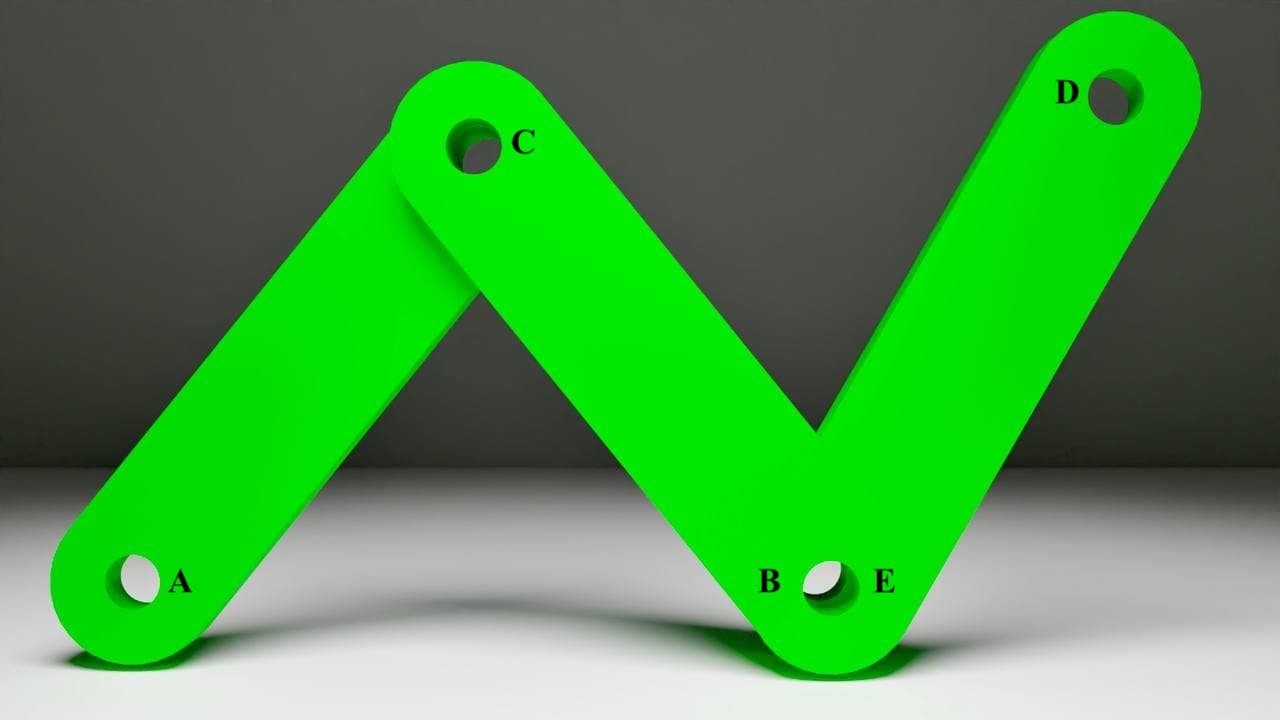
\includegraphics[width=.9\linewidth]{Immagini/Singolarity/4}  
		\label{fig:sing5}
	\end{subfigure}
	\caption{Caso 4 e 5 singolarità}
	\label{Caso4Sing}
\end{figure}
Le soluzioni le possiamo trovare impostando che la lunghezza della x vale nel quarto caso d e nel quinto -d, andando quindi a trovare le soluzioni come:
\begin{equation}
    y_4 = \sqrt{-(x-d)^2}
\end{equation}
e
\begin{equation}
    y_5 = \sqrt{-(x+d)^2}
\end{equation}
Andando ad unire tutti casi visti fino ad ora possiamo vederli visualmente nell'asse $[x,y]$
\begin{figure}[ht]
\begin{center}
    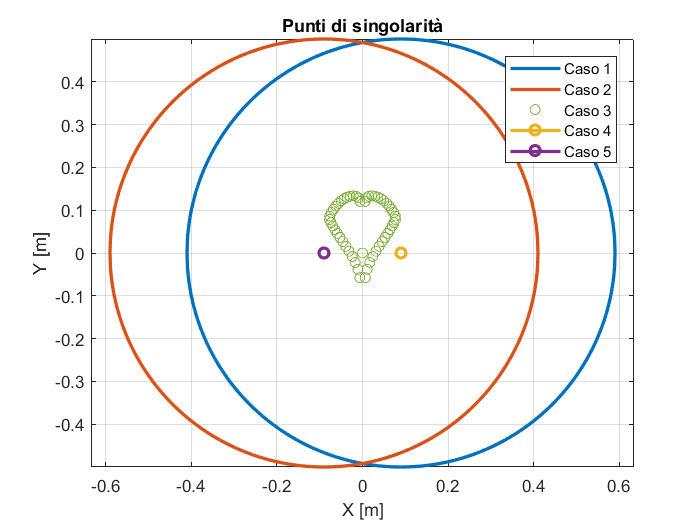
\includegraphics[scale=0.65]{Immagini/Singolarity/SingNew}
    \caption{Punti di singolarità}
    \label{puntiSing}
\end{center}
\end{figure}
\subsection{Manipolabilità}
La manipolabilità ci permette di avere una rappresentazione geometrica delle capacità che ha un punto del nostro sistema. Per andare a calcolarla abbiamo bisogno dell'equazione \ref{eq:J12}, vista nella sezione \ref{sec:CalcoloVelCin}.
\\Andiamo a definire la matrice
\begin{equation}
    J_{man} = JJ^T
\end{equation}
Da questa possiamo ricavare gli autovalori $\Lambda$. Definiamo poi  l'indice di manipolabilità \textbf{r} come:
\begin{equation}
    r = \frac{\max\lambda}{\min\lambda}
\end{equation}
Questo numero può variare tra 1 e $+\infty$, più è piccolo e meno si rischia di andare in singolarità. Possiamo andare a rappresentare il numero di condizionamento tramite i grafici seguenti: 
\begin{figure}[!ht]
	\begin{subfigure}{.55\textwidth}
		\centering
		% include first image
		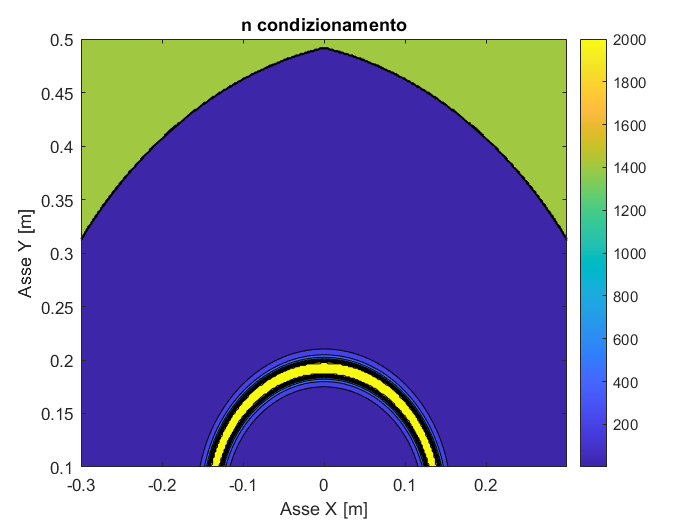
\includegraphics[width=.9\linewidth]{Immagini/Singolarity/Ncond}
		\label{fig:ncond}
	\end{subfigure}
	\begin{subfigure}{.55\textwidth}
		\centering
		% include second image
		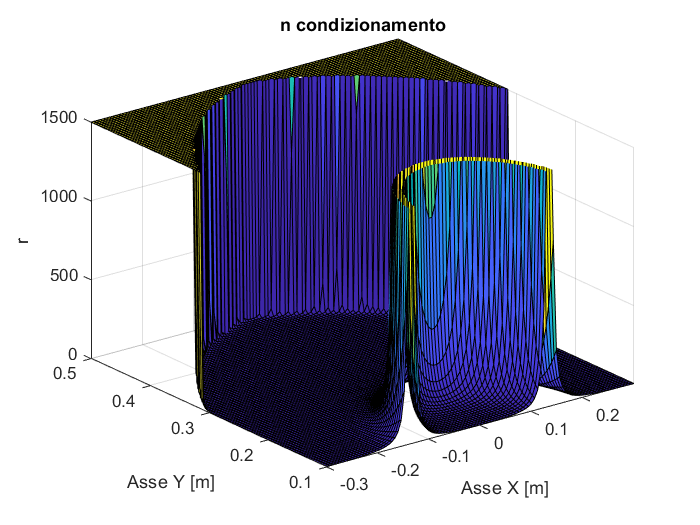
\includegraphics[width=.9\linewidth]{Immagini/Singolarity/Ncond_surf}  
		\label{fig:nconds}
	\end{subfigure}
	\caption{Numero di condizionamento}
	\label{NumCondiz}
\end{figure}
\\Nel primo grafico viene mostrato il piano x,y ed il numero di condizionamento è definito come una colormap, i punti di color blu sono quelli con un r piccolo ed in questi non siamo in condizioni di singolarità, invece quelli tendenti al verde/giallo sono i casi di singolarità che abbiamo visto prima. Nella seconda figura possiamo vedere la stessa rappresentazione però in tre dimensioni, utilizziamo l'asse z per rappresentare il numero di condizionamento; anche qua le zone di singolarità sono chiaramente visibili.
In questo secondo grafico invece andiamo a concentrarci sulla zona di movimentazione ideale del manipolatore, più ci si avvicina allo zero, più il valore di r aumenta, questo per il fatto che stiamo raggiungendo una zona critica.
\subsection{Workspace}
Dalle analisi appena effettuate sui punti di singolarità e sul numero di condizionamento è stato possibile descrivere lo spazio di lavoro del manipolatore. In prima battuta ci si è concentrato sull'analizzare gli angoli di movimentazione dei giunti e i loro vincoli, in particolare il link sinistro con angolo $\theta_1$ avrà una movimentazione di $210^\circ$ al massimo, mentre il link destro con angolo $\theta_2$ ha una movimentazione di $180^\circ$. Questa limitata mobilità è data dai vincoli che ci sono tra le due braccia, infatti, se a livello teorico si possono ottenere configurazioni particolari come quella vista in figura \ref{Caso4Sing} nella pratica non è possibile muovere né manualmente né automaticamente i giunti per ottenere quei casi. Possiamo andare quindi a rappresentare gli angoli di movimentazione mediante la seguente immagine: 
\begin{figure}[ht]
	\begin{center}
		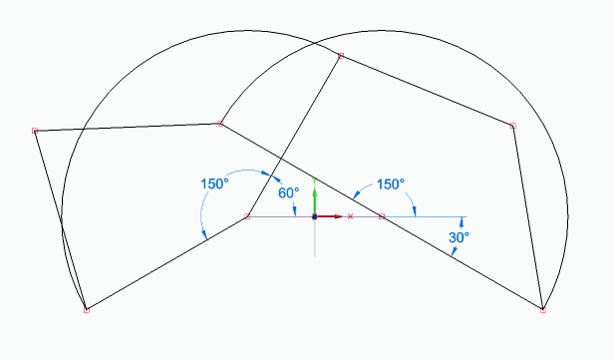
\includegraphics[scale=0.7]{Immagini/Singolarity/workangle}
		\caption{Angoli di movimentazione dei giunti motorizzati}
	\end{center}
\end{figure}
\\Andando ora ad unire gli angoli di movimentazione del manipolatore ed i punti di singolarità, è possibile descrivere lo spazio di lavoro mediante un rettangolo che non viola alcuna condizione
\begin{figure}[ht]
	\begin{center}
		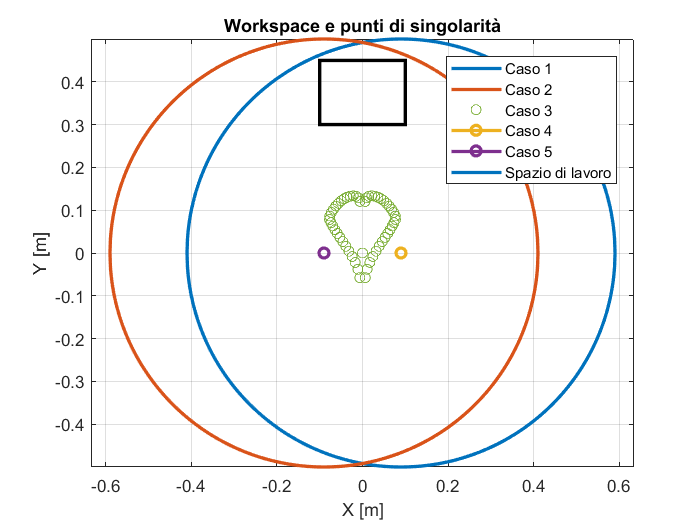
\includegraphics[scale=0.6]{Immagini/Singolarity/Worksing}
		\caption{\textit{Workspace} 5R}
	\end{center}
\end{figure}
\\Successivamente, per verificare che lo spazio di lavoro fosse corretto e rispettasse tutte le condizioni è stata fatta un'analisi sul numero di condizionamento del \textit{workspace}:
\begin{figure}[ht]
	\begin{center}
		\includegraphics[scale=0.6]{Immagini/Singolarity/ncondsl}
		\caption{Numero di condizionamento workspace}
	\end{center}
\end{figure}
\\Su tutto il piano x,y si nota come il numero di condizionamento assume valori bassi, questo implica che non vi è singolarità, gli unici punti critici sono quelli esterni, nei quali il valore è vicino a 6, (comunque minore di $\infty$), questi punti vanno a rappresentare casi nei quali il manipolatore avrà più difficoltà a muoversi, ma non sono veri e propri casi di singolarità.
\section{Analisi cinetostatica}
Una volta effettuata la cinematica e dinamica del sistema in questo capitolo presentiamo l'analisi cinetostatica. In particolare andremo a concentrarci sui punti di singolarità, sul numero di condizionamento e per concludere analizzeremo lo spazio di lavoro del manipolatore.
\begin{figure}[ht]
	\begin{center}
		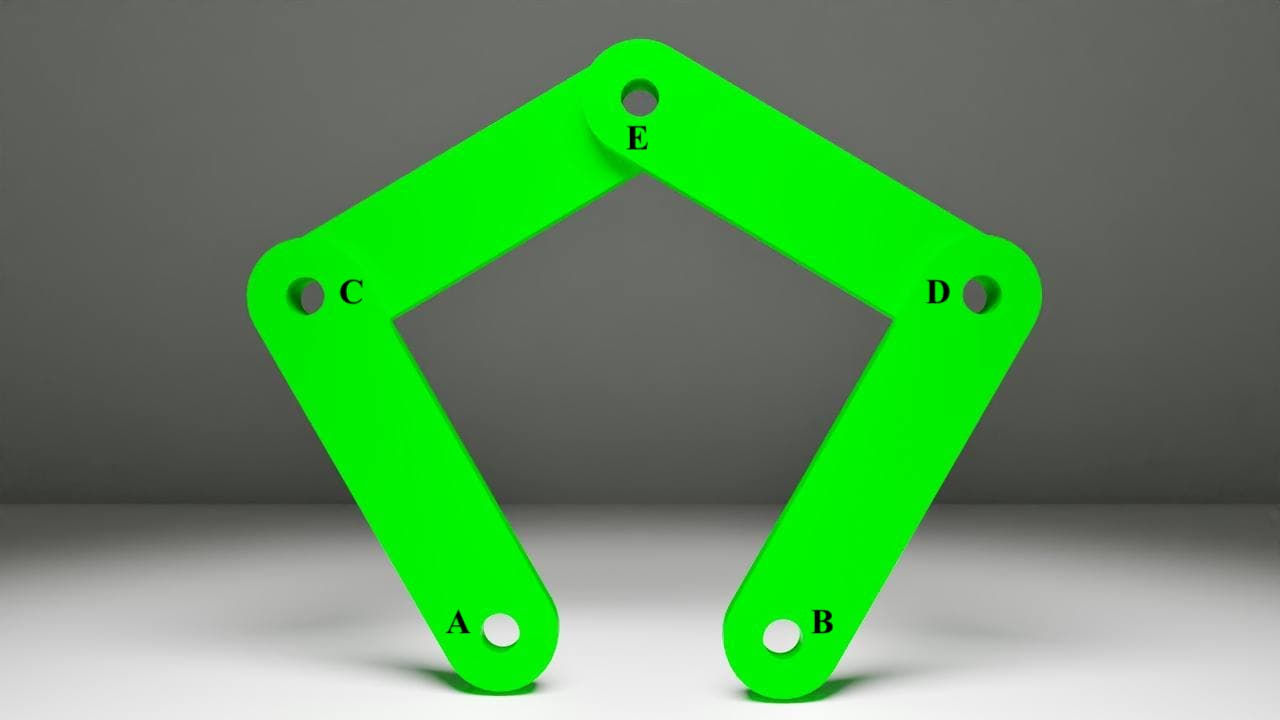
\includegraphics[scale=0.4]{Immagini/Singolarity/0}
		\caption{Posizione standard manipolatore}
	\end{center}
\end{figure}
\subsection{Punti di singolarità}
Nell'ambito matematico, una singolarità è un punto nel quale un oggetto non è definito, oppure un punto nel quale l'oggetto non ha un comportamento normale, nel nostro caso i punti di singolarità sono punti che vanno a delimitare lo spazio di lavoro del robot. Definiamo \textit{workspace} del manipolatore una parte del piano [x,y] nel quale il robot ha un funzionamento normale e non presenta problematiche\footnote{Nel caso in cui il manipolatore dovesse passare per un punto di singolarità potrebbero verificarsi problematiche sia nel seguire la traiettoria che a livello meccanico, arrivando nel peggiore dei casi alla rottura.}. Considerando l'immagine \ref{fig:PKM} si possono identificare cinque casi di singolarità. Di conseguenza il robot avrà come spazio di lavoro, tutto lo spazio che è interno (delimitato) da queste configurazioni.
\subsubsection*{Primo e secondo caso}
\addcontentsline{toc}{subsubsection}{Primo e secondo caso}
In questo primo caso abbiamo $\overrightarrow{CD}$ che è parallelo a $\overrightarrow{DE}$, schematicamente possiamo andarlo a rappresentare nel seguente modo
\begin{figure}[ht]
	\begin{center}
		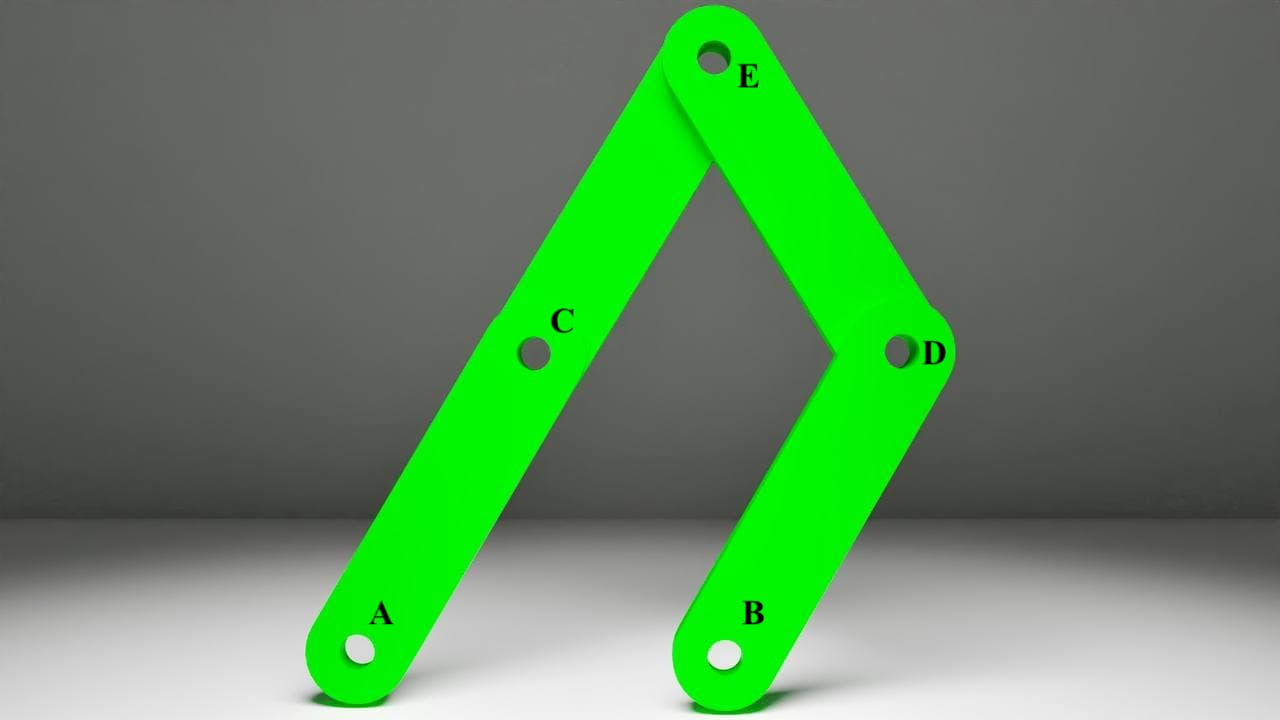
\includegraphics[scale=0.4]{Immagini/Singolarity/1}
		\caption{Caso 1 singolarità}
	\end{center}
\end{figure}
\\Analiticamente: $||\overrightarrow{AC}||^2 = (l+l)^2$ quindi: 
\begin{equation*}
	\Bigg| \begin{bmatrix}
		-d  \\ 0
	\end{bmatrix} - \begin{bmatrix}
	x \\ y
\end{bmatrix}\bigg|^2 = 4l^2
\end{equation*}
\begin{equation*}
\bigg|	\begin{bmatrix}
		-d-x \\ -y
	\end{bmatrix}\Bigg|^2 = 4l^2
\end{equation*}
Svolgendo il modulo troviamo 
\begin{equation*}
	d^2 + 2dx + x^2 +y^2 = 4l^2
\end{equation*}
Facendo variare x ricaviamo la y come:
\begin{equation}
    y_1 = \sqrt{4l^2-(x-d)^2}
\end{equation}
Per quanto riguarda il secondo caso è simmetrico al primo, abbiamo la catena $\overrightarrow{AB}$ parallela a $\overrightarrow{BC}$:
\begin{figure}[ht]
	\begin{center}
		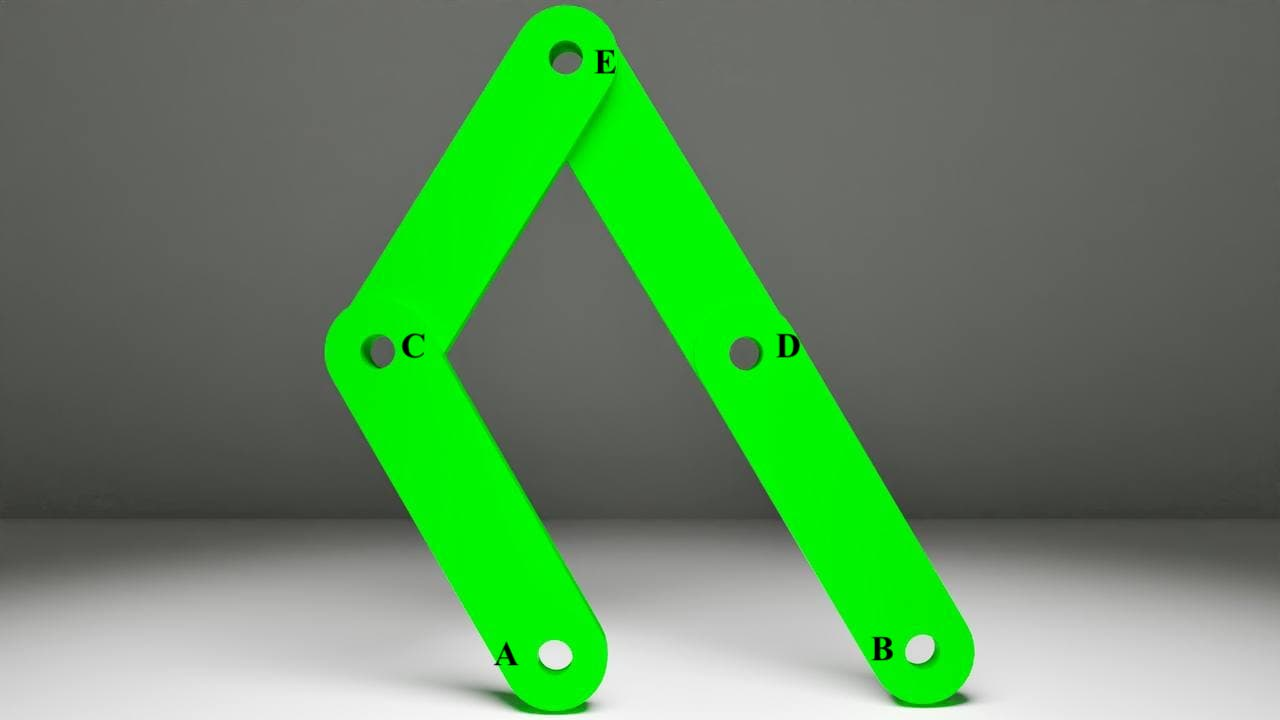
\includegraphics[scale=0.4]{Immagini/Singolarity/2}
		\caption{Caso 2 singolarità}
	\end{center}
\end{figure}
\\Il procedimento è simile a prima, lasciando sempre la x libera possiamo trovare la y come:
\begin{equation}
    y_2 = \sqrt{4l^2-(x+d)^2}
\end{equation}
Entrambi i casi producono come risultato una circonferenza.
\subsubsection*{Terzo caso}
\addcontentsline{toc}{subsubsection}{Terzo caso}
Il terzo caso di singolarità avviene quando i due link non motorizzati sono paralleli, abbiamo tre giunti allineati tra di loro rendendo la configurazione labile. Per poter uscire da questa singolarità abbiamo la necessità di una maggior coppia.
\begin{figure}[ht]
	\begin{center}
		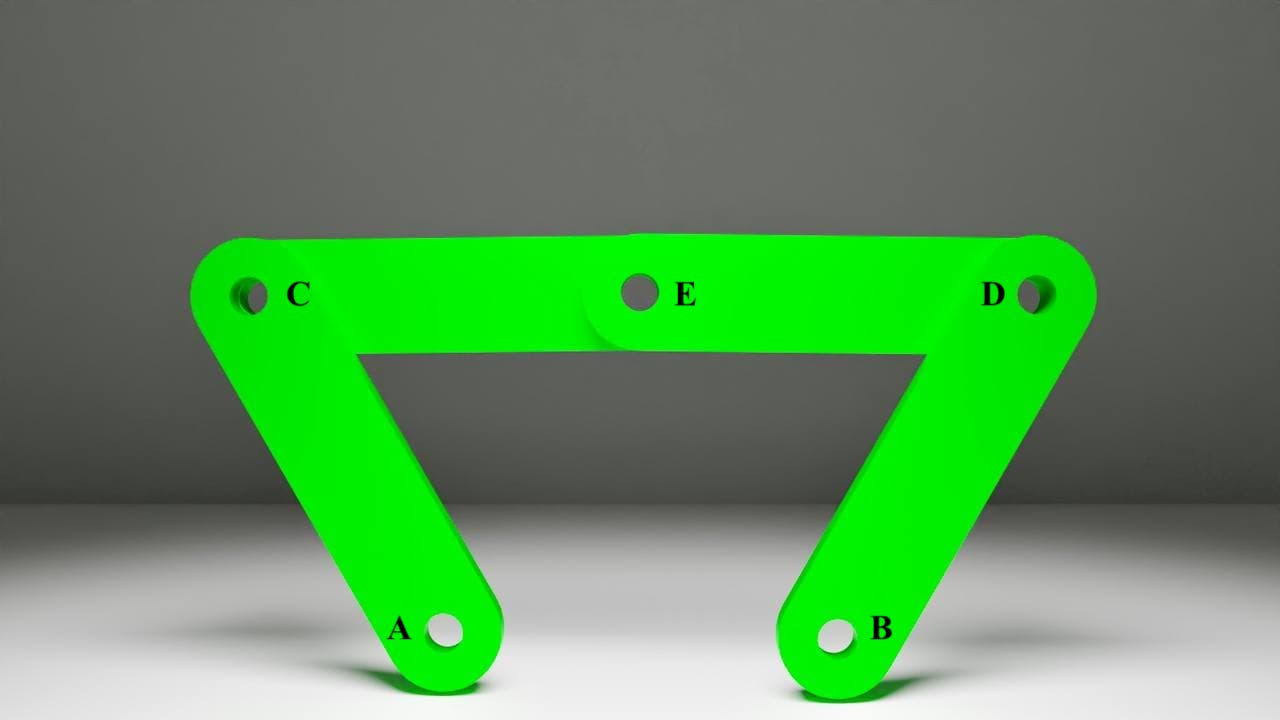
\includegraphics[scale=0.4]{Immagini/Singolarity/5}
		\caption{Caso 3 singolarità}
	\end{center}
\end{figure}
\\Per quanto riguarda la soluzione, andiamo inizialmente a trovare la posizione del punto D $[x_D,y_D]$: facciamo l'intersezione tra due circonferenze la prima ha centro in E con raggio l, la seconda ha centro in B con raggio 2l; possiamo esprimere le equazioni come:
\begin{equation}
	\begin{cases}
		(x_D-d)^2 +y_D^2= l \\
		(x_D-l\cos\theta_1+d)^2 + (y_D-l\sin\theta_1)^2 = 4l^2
	\end{cases}
\end{equation}
Svolgendo i quadrati:
\begin{equation*}
	\begin{cases}
	 x_D^2-2dx_D+d^2+y_D^2 = l^2 \\
	 x_D^2+ l^2 + d^2-2ld\cos\theta_1 -2x_Dl\cos\theta_1+2x_Dd + y_D^2-2y_Dl\sin\theta_1 = 4l^2-l^2
	\end{cases}
\end{equation*}
Sottraendo la prima equazione nella seconda otteniamo: 
\begin{equation*}
	x_D(-l\cos\theta_1+2d) -y_Dl\sin\theta_1 - ld\cos\theta_1 = l^2
\end{equation*}
Otteniamo x in funzione di y come:
\begin{equation*}
	x_{D} = \frac{l^2+y_{D}l\sin\theta_1+ld\cos\theta_1}{2d-l\cos\theta_1}
\end{equation*}
 Sostituendo la x nella prima equazione possiamo ottenere y in funzione di $\theta_1$:
 \begin{equation}
 	y_{D} = \frac{-b\pm \sqrt{b^2-4ac}}{2a}
 \end{equation}
 dove:
\begin{equation*}
	a = l^2\sin^2\theta_1 + 4d^2-4dl\cos\theta_1 + l^2\cos^2\theta_1
\end{equation*}
\begin{equation*}
	b = 2l^3\sin\theta_1 + 2dl^2\sin\theta_1\cos\theta_1-2dl\sin\theta_1(2d-2l\cos\theta_1)
\end{equation*}
\begin{equation*}
	c = l^2(l^2+d^2\cos^2\theta_1+2ld\cos\theta_1)-2dl(l+d\cos\theta_1)(2d-l\cos\theta_1)+(d^2-l^2)(2d-l\cos\theta_1)^2
\end{equation*}
Facendo variare $\theta_1$ troviamo $x_D$ e $y_D$. Per poter trovare la posizione dell'\textit{end-effector} facciamo la media tra la posizione del punto D e del punto B.
\begin{equation}
	x_3 = \frac{x_D-d+l\cos\theta_1}{2}, y_3 = \frac{y_B+l\sin\theta_1}{2}
\end{equation}
\subsubsection*{Quarto e quinto caso}
\addcontentsline{toc}{subsubsection}{Terzo e quarto caso}
Il quarto e quinto sono casi di singolarità non realizzabili nella pratica, ma sono di interesse teorico. Il primo prevede che la posizione dell'end-effector coincida con la posizione del primo giunto motorizzato mentre nell'altro che coincida con il secondo giunto motorizzato. Come soluzioni avremo semplicemente due punti e possiamo andare a calcolarli nei seguenti modi:
\begin{figure}[!ht]
	\begin{subfigure}{.5\textwidth}
		\centering
		% include first image
		
\includegraphics[width=.9\linewidth]{Immagini/Singolarity/3}
		\label{fig:sing4}
	\end{subfigure}
	\begin{subfigure}{.5\textwidth}
		\centering
		% include second image
		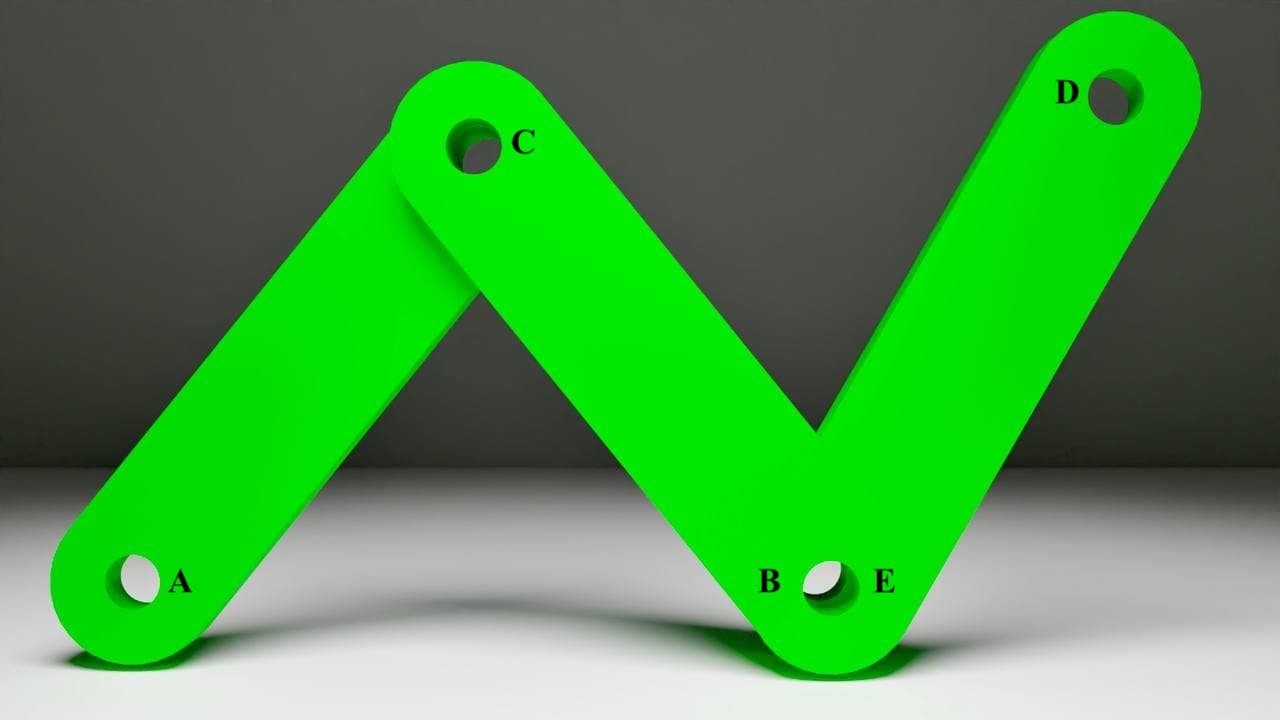
\includegraphics[width=.9\linewidth]{Immagini/Singolarity/4}  
		\label{fig:sing5}
	\end{subfigure}
	\caption{Caso 4 e 5 singolarità}
	\label{Caso4Sing}
\end{figure}
\\Possiamo trovare le soluzione del quarto caso imponendo \begin{equation}|\overrightarrow{EC}| = 0 \rightarrow x=d, y = 0
\end{equation}
e per il quinto caso 
\begin{equation}
	|\overrightarrow{AC}| = 0 \rightarrow x=-d, y=0
\end{equation}
Per delimitare i confini di operabilità del manipolatore sono stati uniti tutti e cinque i casi di singolarità. Nella figura seguente è fornita una rappresentazione sul piano cartesiano dell'unione di questi luoghi di singolarità, facciamo notare che non tutti i punti sono fisicamente raggiungibili dal robot per come è stato progettato; in particolare la posizione y dell'\textit{end-effector} non potrà mai essere negativa.
\begin{figure}[ht]
\begin{center}
    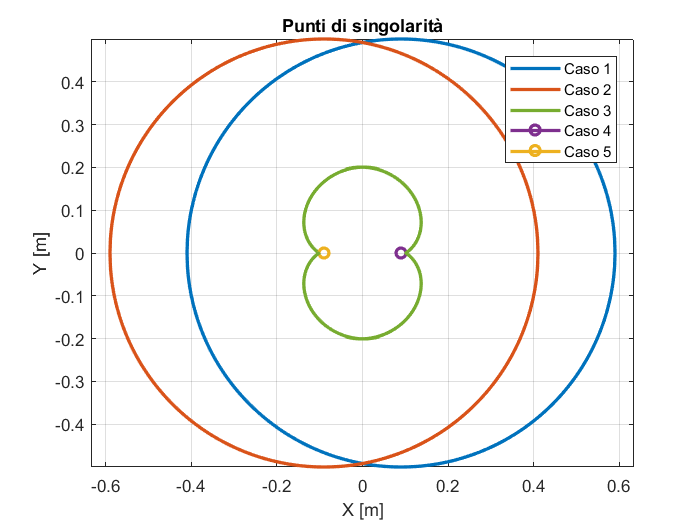
\includegraphics[scale=0.65]{Immagini/Singolarity/SingNewNew}
    \caption{Punti di singolarità}
    \label{puntiSing}
\end{center}
\end{figure}
\subsection{Manipolabilità}
La manipolabilità ci permette di avere una rappresentazione geometrica delle capacità che ha un punto del nostro sistema. Per andare a calcolarla abbiamo bisogno dell'equazione \ref{eq:J12}, vista nella sezione \ref{sec:CalcoloVelCin}.
\\Andiamo a definire la matrice
\begin{equation}
    J_{man} = JJ^T
\end{equation}
Da questa possiamo ricavare gli autovalori $\lambda_1, \lambda_2$. Definiamo  l'indice di manipolabilità \textbf{r} come:
\begin{equation}
    r = \frac{\max(\lambda_1,\lambda_2)}{\min(\lambda_1,\lambda_2)}
\end{equation}
Questo numero può variare tra 1 e $+\infty$, più è piccolo e meno si rischia di andare in singolarità. Lo spazio analizzato ha come estremi:
\begin{equation*}
	\begin{split}
		-0.3 \le x \le 0.3 \\
		0.1 \le y \le 0.5
	\end{split}
\end{equation*} 
Rappresentiamo il numero di condizionamento tramite i seguenti grafici: 
\begin{figure}[!ht]
	\begin{subfigure}{.55\textwidth}
		\centering
		% include first image
		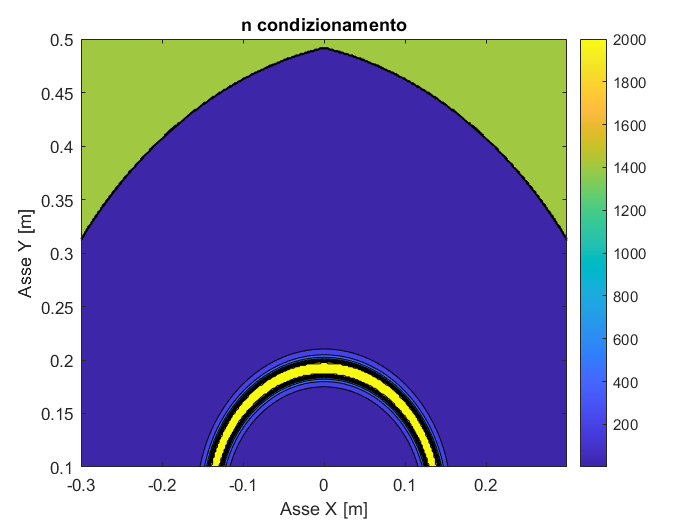
\includegraphics[width=.9\linewidth]{Immagini/Singolarity/Ncond}
		\label{fig:ncond}
	\end{subfigure}
	\begin{subfigure}{.55\textwidth}
		\centering
		% include second image
		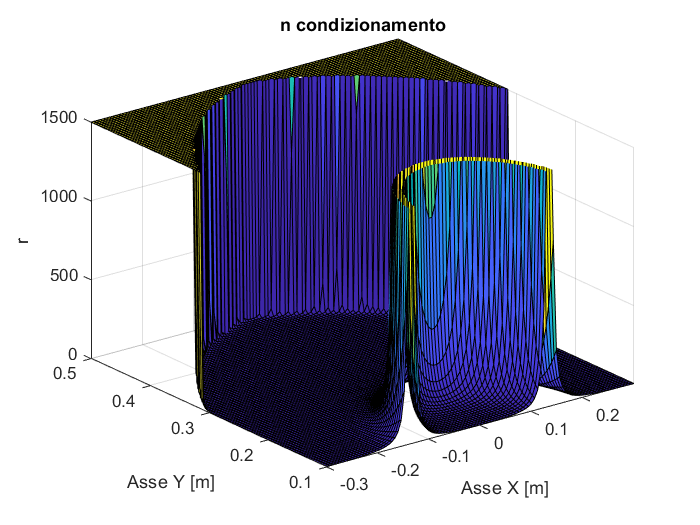
\includegraphics[width=.9\linewidth]{Immagini/Singolarity/Ncond_surf}  
		\label{fig:nconds}
	\end{subfigure}
	\caption{Numero di condizionamento}
	\label{NumCondiz}
\end{figure}
\\Nel primo grafico viene mostrato il piano x,y ed il numero di condizionamento è definito come una colormap, i punti di color blu sono quelli con un r piccolo ed in questi non siamo in condizioni di singolarità, invece quelli tendenti al verde/giallo sono i casi di singolarità che abbiamo visto prima. Nella seconda figura possiamo vedere la stessa rappresentazione però in tre dimensioni, utilizziamo l'asse z per rappresentare il numero di condizionamento; anche qua le zone di singolarità sono chiaramente visibili.

\subsection{Workspace}
Dalle analisi appena effettuate sui punti di singolarità e sul numero di condizionamento è stato possibile descrivere i limiti di lavoro del manipolatore. In prima battuta ci si è concentrato sull'analizzare gli angoli di movimentazione dei giunti e i loro vincoli, in particolare il link sinistro con angolo $\theta_1$ può effettuare un movimento da $60^\circ$ fino a $210^\circ$, mentre il link destro da $-30^\circ$ e $150^\circ$. Questa limitata mobilità è data dai vincoli che ci sono tra le due braccia, infatti, se a livello teorico si possono ottenere configurazioni particolari come quella vista in figura \ref{Caso4Sing} nella pratica non è possibile muovere né manualmente né automaticamente i giunti per ottenere quei casi, l'unico modo possibile è quello di smontare e rimontare il manipolatore al contrario. \\Possiamo andare a rappresentare gli angoli di movimentazione mediante la seguente immagine: 
\begin{figure}[ht]
	\begin{center}
		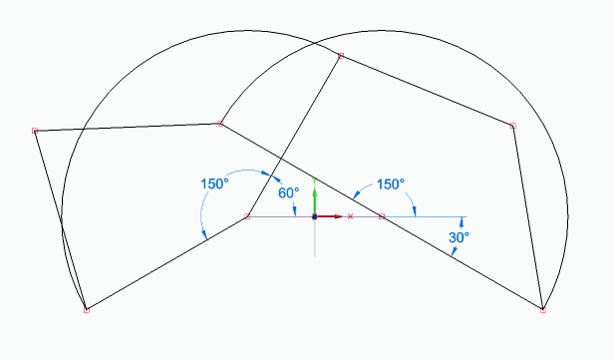
\includegraphics[scale=0.7]{Immagini/Singolarity/workangle}
		\caption{Angoli di movimentazione dei giunti motorizzati}
	\end{center}
\end{figure}
\\A partire dai limiti di lavoro è stato identificato uno spazio buono dove il manipolatore può operare non raggiungendo i punti singolari. Questo luogo è stato descritto mediante un rettangolo:
\begin{figure}[ht]
	\begin{center}
		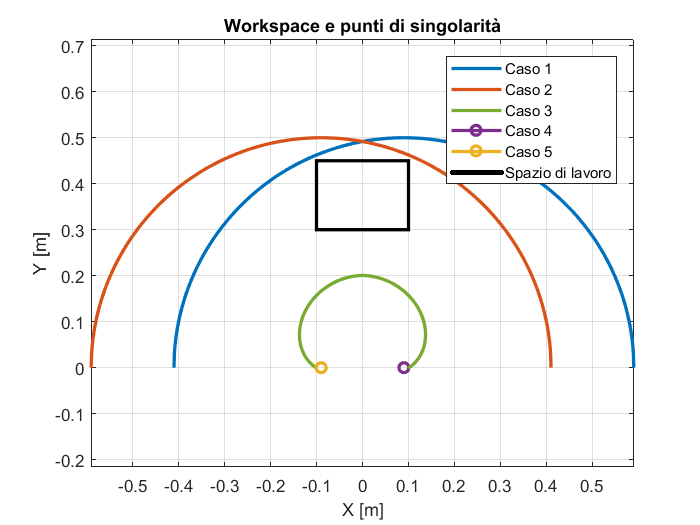
\includegraphics[scale=0.6]{Immagini/Singolarity/WorksingNew}
		\caption{\textit{Workspace} 5R}
	\end{center}
\end{figure}
\\Con estremi:
\begin{equation*}
	\begin{split}
		-0.1 \le x \le 0.1 \\
		0.3 \le y \le 0.45
	\end{split}
\end{equation*}
\\Successivamente, per verificare che lo spazio di lavoro fosse corretto e rispettasse tutte le condizioni è stata fatta un'analisi sul numero di condizionamento del \textit{workspace}:
\begin{figure}[ht]
	\begin{center}
		\includegraphics[scale=0.6]{Immagini/Singolarity/ncondsl}
		\caption{Numero di condizionamento workspace}
	\end{center}
\end{figure}
\\Su tutto il piano x,y si nota come il numero di condizionamento assume valori bassi, questo implica che non vi è singolarità, gli unici punti critici sono quelli esterni, nei quali il valore è vicino a 6, (comunque minore di $\infty$), questi punti vanno a rappresentare casi nei quali il manipolatore avrà più difficoltà a muoversi, ma non sono veri e propri punti di singolarità.
\section{Modellazione end-effector}
L'obiettivo di questo capito consiste nel presentare la modellazione della cinematica e dinamica dell'end-effector.
\\L'end-effector, denominato anche come utensile, è composto da due componenti, azionati da due motori, il primo componente è una vite a ricircolo di sfere, il secondo invece è una guida lineare. 
\begin{table}[h!]
\centering
\begin{tabular}{|c |c |c|} 
 \hline
 Nome & Descrizione  & Valore \\ [0.5ex] 
 \hline\hline
 $m_v [kg]$ & massa vite  & 0.36 \\ 
 $p_v [m]$ & passo vite & 0.02 \\
 $I_v [kg\cdot m^2]$ & momento inerzia vite  & $6.40\cdot 10^{-6}$ \\
 \hline
\end{tabular}
\caption{Parametri end-effector}
\label{table:2}
\end{table}
A livello teorico si è partito definendo una legge di modo per i due componenti dell'end-effector, per entrambi la legge è polinomiale, la differenza però sta nel fatto che per la guida la facciamo sulla posizione mentre per la vite sull'orientamento.
\subsection{Cinematica end-effector}
Come abbiamo anticipato nell'introduzione di questa sezione abbiamo la presenza di due leggi di moto che andiamo a chiamare $z_ee$ e $\varphi_v$. Da queste condizioni iniziali dobbiamo ricavare la cinematica di posizione, andiamo quindi ad introdurre la Jacobiana dell'end-effector in questo modo: 
\begin{equation*}
J_e =
    \begin{bmatrix}
    \frac{p_v}{2\cdot \pi} & \frac{p_v}{2\cdot \pi} \\
    0 & 1
    \end{bmatrix}
\end{equation*}
Andiamo ora ad introdurre la variabile V con le sue rispettive derivate, che saranno i risultati della cinematica diretta di posizione, velocità ed accelerazione:
\begin{equation*}
    V = 
    \begin{bmatrix}
     Z \\ 
     \theta_Z
    \end{bmatrix}, 
    \dot{V} = 
    \begin{bmatrix}
    \dot{Z} \\ \dot{\theta_Z}
    \end{bmatrix},
    \ddot{V} =
    \begin{bmatrix}
    \ddot{Z} \\ \ddot{\theta_Z}
    \end{bmatrix}
\end{equation*}
Per concludere andiamo ad eseguire le operazione di cinematica diretta in questo modo:
\begin{equation}
    V = J_e\cdot \begin{bmatrix}
    z_{ee} \\ \varphi_v
    \end{bmatrix},
    \dot{V} = J_e\cdot \begin{bmatrix}
    \dot{z_{ee}} \\ \dot{\varphi_v}
    \end{bmatrix},
    \ddot{V} = J_e\cdot \begin{bmatrix}
    \ddot{z_{ee}} \\ \ddot{\varphi_v}
    \end{bmatrix}
\end{equation}

\subsection{Dinamica della vite}
Per la definizione della dinamica della vite come tecnica è stata usata quella del PLV, come è stato fatto anche per la modellazione della dinamica dei bracci. 
\begin{equation*}
    inserire equazione?
\end{equation*}
Da questa si nota che abbiamo bisogno delle accelerazioni dei due elementi, andando a sviluppare i calcoli otteniamo la coppia come segue:
\begin{equation}
    C_ee = \begin{bmatrix}
    m_e & 0 \\ 0 & I_v
    \end{bmatrix}
    \cdot J_e\cdot \begin{bmatrix}
    \ddot{z_{ee}} \\ \ddot{\varphi_v}
    \end{bmatrix}
\end{equation}
Nella seguente immagine è possibile vedere il risultato di questo calcolo, con ingresso la legge di moto polinomiale
\begin{figure}[ht]
\begin{center}
    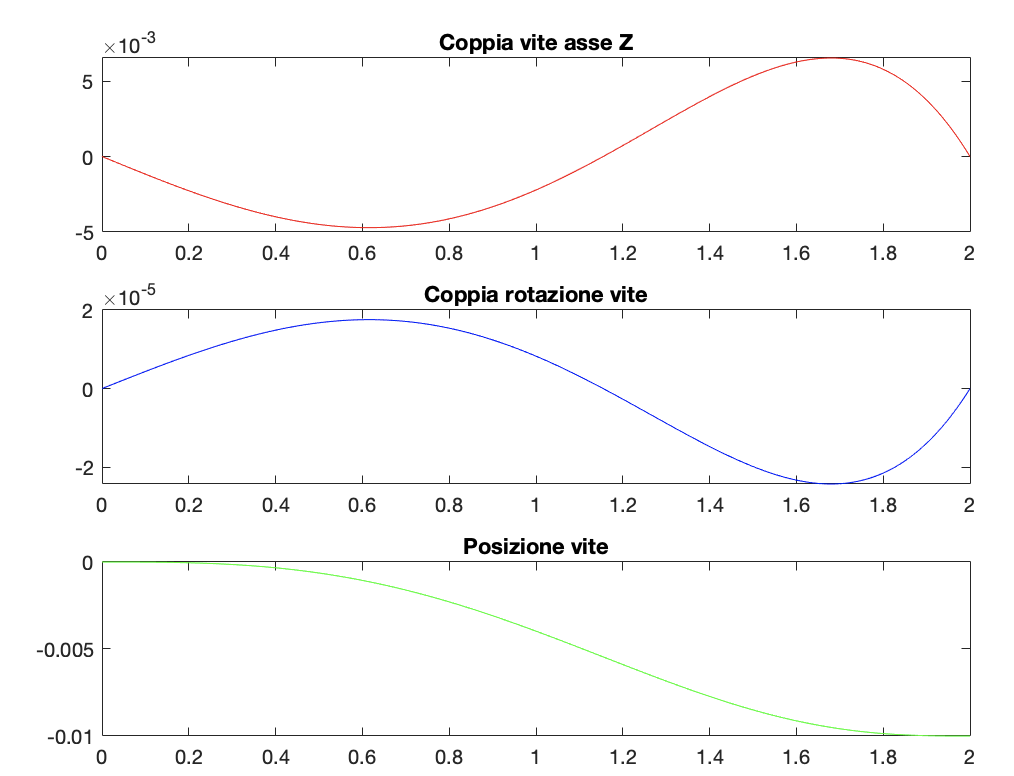
\includegraphics[scale=0.55]{Immagini/coppiaTeoricaVite.png}
    \caption{Coppie e posizione end-effector}
\end{center}
\end{figure}
In particolare sono mostrate le coppie dei due componenti e la posizione finale dell'end-effector
\subsection{Modellazione su Adams}
\newpage
\thispagestyle{plain} % empty
\mbox{}
\section{Tecnologie implementate}
Conclusa la spiegazione della modellazione di bracci e vite è il momento di iniziare l'attività sperimentale. Lo scopo di questa sezione è l'introduzione alle tecnologie software utilizzate per la modellazione fisica del manipolatore.
\subsection{Simulink Real time}
Simulink real-time è un plugin di matlab, consente di creare applicazioni real-time ed eseguirle su un hardware target, come per esempio un computer. Simulink-real time gira su un computer di "sviluppo" che è il PC utente, ed è diverso dal sistema che permette il movimento in real-time e l'esecuzione del modello reale ovvero il dispositivo target. Di conseguenza simulink real-time può raggiungere tempi di campionamento molto più veloci per uno stesso modello rispetto ad kernel real-time che condivide le risorse hardware con il computer, vi è la possibilità di raggiungere anche i 20 kHz. 
Un'altra caratteristica fondamentale è il fatto che su SLRT è possibile far funzionare il dispositivo target in modalità \textit{stand-alone} cioè può riuscire ad avviarsi senza il bisogno di una procedura di installazione. 

\subsection{EtherCAT}
L'obiettivo di questa sottosezione è quello di presentare il protocollo di comunicazione utilizzato per interfacciarsi col robot PKM, evidenziandone le sue caratteristiche principali.\\
EtherCAT è una tecnologia ethernet sviluppata in origine da Beckhoff automation, il protocollo è stato pubblicato nello standard IEC61158\footnote{${https://webstore.iec.ch/publication/59890}$}, soddisfa requisiti \textit{hard} e \textit{soft} real time in particolare nell'ambito dell'automazione. Una caratteristica particolare sono i tempi di ciclo che sono molto veloci infatti una durata media di un tempo di ciclo è inferiore a $100 \mu s$. Il principio base di funzionamento si basa sul concetto di \textit{Master/Slave}.
\\ Venne introdotto nell'aprile 2003, e nei mesi successivi è nata una società chiamata EtherCAT Technology Group (ETG) che è diventata una delle più grandi organizzazioni ethernet al mondo.
\subsubsection{Proprietà}
%\addcontentsline{toc}{subsubsection}{Proprietà}
Il master EtherCAT invia un pacchetto, chiamato telegramma che va ad attraversare tutti i nodi, ogni singolo slave collegato legge i dati che riguardano lui e scrive i dati prodotti intanto che il telegramma si propaga sulla rete verso i nodi successivi. Non appena il pacchetto arriva all'ultimo nodo, è quest'ultimo che si occupa di reinviarlo al master grazie alla comunicazione full-duplex presa da Ethernet, facendo questo, il flusso di dati teorico riesce a superare i $100 Mbit/s$. Il fatto che il master sia l'unico nodo che può inviare frame in maniera attiva garantisce prestazioni deterministiche.\\ Il master utilizza un Media Access Controller (MAC) standard, senza alcun processore dedicato alla comunicazione. Questo consente di implementare un dispositivo master su qualunque piattaforma hardware dotata di una porta di rete, indipendentemente dal Sistema Operativo o software applicativo utilizzato. I dispositivi EtherCAT slave integrano un cosiddetto EtherCAT Slave Controller (ESC) in grado di processare i frame on-the-fly e in modo puramente hardware, il che rende le prestazioni della rete predicibili e indipendenti dalla particolare implementazione dei dispositivi slave.
\subsubsection{Gestione della rete}
La rete EterCAT è sicura, viene implementato una tecnologia denominata \textit{safety over EtherCAT} che consente la realizzazione di architetture di sicurezza più semplici e flessibili di una logica standard a relè. Vi è la possibilità di trovare questa tecnologia standardizzata nella specifica IEC 61784-3, il sistema di comunicazione è parte del \textit{black channel}, ovvero una parte considerata non rilevante ai fini della sicurezza; questo fa uso di un solo canale per trasferire sia i dati standard che quelli di sicurezza, i frame di sicurezza vengono identificati come \textit{safety container}, e contendono i dati critici del processo e l'informazione necessaria per garantirne l'integrità. Un \textit{safety container} viene mappato dentro i dati di processo ciclici di comunicazione, possono viaggiare tramite cavi di rame, fibre ottiche e connessioni \textit{wireless}, questo introduce flessibilità, e rende più semplice e sicuro connettere parti della macchina anche lontane fra di loro. In una macchina completamente connessa, andare ad implementare una funzione d'arresto di emergenza totale risulterà semplice anche se altre parti della macchina sono connesse con tecnologie diverse. 
\subsubsection{Implementazione interfacce}
Come abbiamo accennato precedentemente, il principio di funzionamento di \textit{EtherCAT} è il concetto di \textit{master/slave}. Per come si è evoluta questa tecnologia, e considerando che l'interfaccia non richiede una CPU ad elevate prestazioni, è possibile andare ad aggiungere un dispositivo di I/O ad un controllore senza andare ad aumentare significativamente i costi complessivi. Per un cliente, è importante l'interoperabilità tra i dispositivi di più fornitori, per questo prima di poter introdurre un dispositivo sul mercato vengono fatti tutti i test, che verificano che l'implementazione rispetti la specifica EtherCAT.\\ L'interfaccia master ha l'unico requisito di avere una porta ethernet, per l'implementazione viene utilizzato o l'ethernet controller integrato oppure una schede di rete base; nella maggior parte dei casi l'ethernet controller viene integrato mediante un DMA (Direct Memory Access), in questo modo per l'invio dei dati tra il master e la rete non vengono utilizzare le risorse della CPU. Gli slave scrivono i dati prodotti e leggono quelli a loro indirizzati mentre il telegramma li attraversa, facendo così al master arriva l'immagine già ordinata correttamente, la CPU quindi non è più responsabile dell'ordinamento. I dispositivi \textit{slave} invece utilizzano ESC (\textit{Ethercat slave controller)}, solitamente di costo contenuto oppure integrato in un microcontrollore standard, esistono slave semplici che non richiedono nemmeno la presenza di un microcontrollore per il fatto che gli ingressi e le uscite digitali possono essere direttamente collegati all'ESC, mentre per quelli più complessi viene usato un controllore a 8-bit.
\subsection{CME2}
CME2 è un software prodotto da Copley control, e serve per la configurazione degli azionamenti. Le funzioni principali riguardano \textit{auto-phasing} e \textit{auto-tuning}, che vanno a semplificare la realizzazione del sistema. Oltre a queste due funzioni principali abbiamo anche le tabelle Cam che forniscono un buon approccio per la produzione di movimenti sincronizzati e ripetitivi ad un dispositivo esterno, e la possibilità di definire sequenze fino a 32 indici o sequenze indicizzate. Sono anche predisposte funzioni per l'analisi degli strumenti, la configurazione dei motori dei filtri e dei guadagni, è possibile anche andare a cambiare la modalità operativa, scegliendo quindi se lavorare con un anello in posizione, corrente o coppia. Il collegamento con gli azionamenti è avvenuto tramite cavo ethernet, 
\begin{figure}[ht]
\begin{center}
    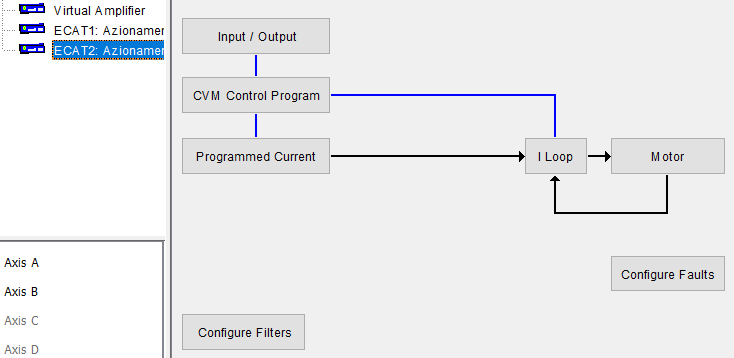
\includegraphics[scale=0.8]{Immagini/Sperimentale/azionamenti.PNG}
    \caption{Schema azionamento}
\end{center}
\end{figure}
come si può notare dalle foto gli azionamenti sono controllati in corrente. Un'operazione fondamentale è stata l'analisi dei registri nella quale si è visto a cosa corrispondeva ogni registro. In particolare i registri osservati sono stati quelli dei finecorsa.
Per le braccia i registri da guardare sono stati l'ottavo e il quindicesimo, in particolare per vincoli di progetto i finecorsa osservati sono stati quelli al lato destro, per la vite invece il registro osservato è stato il quindicesimo, ed era riferito alla movimentazione superiore della vite.
\begin{figure}[ht]
\begin{center}
    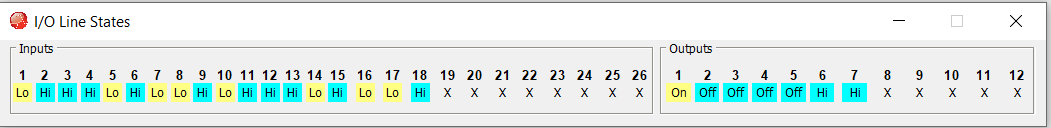
\includegraphics[scale=0.6]{Immagini/Sperimentale/registri.PNG}
    \caption{Registri azionamento}
\end{center}
\end{figure}
\subsection{EC-Engineer}
EC-Engineer è uno strumento software utilizzato per la configurazione, diagnostica e monitoraggio delle reti EtherCAT, è nato con lo scopo di aver tutto il necessario su un solo ambiente. Usando questo programma è possibile generare due tipologie di configurazioni EtherCAT, online oppure offline. Il primo tipo di configurazione viene fatto quando siamo direttamente connessi sulla macchina alla rete EtherCAT quindi è un'operazione fatta in real-time, la sconda tipologia invece può essere fatta in laboratorio o ufficio e non richiede la connessione alla rete in quel preciso momento. Per andare a fare una connessione online non è necessario che gli slave siano direttamente connessi al PC locale, questo grazie alla funzione \textit{bus scan} che permette di andare a determinare la topologia della rete facilmente. Nel nostro caso abbiamo scelto una configurazione \textit{offline}, come metodo di comunicazione si è scelto di usare le PDO\footnote{\textit{Process Data Object}, ovvero dati trasmetti dal/al \textit{MotionController}, in tempo reale ad ogni nodo ad ogni tempo di campionamento.}. Per concludere la configurazione viene esportato un file ENI,
ovvero un file XML che descrive la topologia della rete, il comando di inizializzazione per ogni dispositivo ed i comandi che devono essere inviati ciclicamente, il file ENI viene fornito al master che invia i comandi in base a questo file. Una volta creato è stato inserito su simulink nell'\textit{EtherCAT init}.

\newpage
\thispagestyle{plain} % empty
\mbox{}
\section{Sistema reale}
Avendo introdotto anche le tecnologie implementate, andiamo ora a discutere del sistema reale, in particolare concentrandoci sulla sua struttura, compresa la configurazione, le operazioni che hanno consentito la movimentazione e le tecniche di controllo
\subsection{Struttura del robot}
Il manipolatore PKM è un manipolatore a cinematica parallela, composto da due braccia ed un end-effector. Alle braccia sono collegati due motori, uno per il link motorizzato sinistro e l'altro per il link motorizzato destro, i link distali si muovono in conseguenza al movimento di quelli motorizzati. Anche l'end-effector è composto da due motori, il primo motore permette di far salire/scendere la vite, il secondo invece genera un moto elicoidale che permette la rotazione della vite con conseguente salita/discesa. 
Per quanto riguarda la parte elettronica abbiamo la presenza di due azionamenti che sono collegati uno ai motori delle braccia e l'altro ai motori della vite ed un modulo beckhoff che si occupa della gestione degli input digitali.
\begin{figure}[ht]
	\begin{center}
		\includegraphics[scale=0.6]{Immagini/Sperimentale/banco}
		\caption{Banco di test}
		\label{fig:BancoProva}
	\end{center}
\end{figure}
Per funzionare il sistema ha bisogno di due alimentatori, uno che serve ad alimentare la logica,alimentato a 24 Volt e un altro che serve ad alimentare i quattro motori, 80 Volt.
\subsubsection{Azionamenti}
Gli azionamenti utilizzati sono gli accelnet plus a 2 assi BE2, sono progettati appositamente per EtherCAT, operano con tensioni da 14 a 90 volt, riescono a fornire in uscita fino a 30A.
\\Sono predisposti per controllo in posizione, velocità e coppia di motori brushless, per la configurazione utilizzano il software CME 2 e la comunicazione avviene mediante l'interfaccia seriale RS-232. Il BE2 opera come ethercat slave, utilizzando il layer applicativo CAN su ethercat CoE. Inoltre, viene fornito un input AuxHV che permette in casi critici di tener vivo l'azionamento anche quando non c'è alimentazione senza perdere le informazioni sulla posizione o le comunicazioni con il sistema di controllo.
Per la comunicazione con ethercat invece sono predisposti due cavi RJ-45, la porta d'ingresso IN permette la connessione ad un master o alla porta d'uscita OUT di un dispositivo che nella gerarchia è interposto tra il master e l'azionamento. Inoltre, se l'accelnet è l'ultimo nodo della rete non vi è bisogno di un terminatore sulla porta d'uscita.
 
\subsubsection{Beckhoff EK1814}
Il beckhoff EK1814 è un accoppiatore EtherCAT che fa da \textit{link} tra il protocollo EtherCAT a livello di bus di campo e il terminali EtherCAT. Inoltre, su questo modello sono anche integrati quattro input digitali e quattro output digitali. La sua struttura lo rende ideale per applicazioni con pochi input/output. L'accoppiatore converte i telegrammi che passano da Ethernet \textit{100BASE-TX} a rappresentazioni di segnali \textit{E-bus}. Una stazione EtherCAT è formata da un accoppiatore e da un numero N di terminali che vengono identificati automaticamente.
\\Inoltre, l'EK1814 ha due connessioni RJ45, l'interfaccia Ethernet superiore è utilizzata per collegare l'accoppiatore alla rete, mentre quella posteriore serve per il collegamento di altri dispositivi EtherCAT nello stesso commento. Nel nostro progetto è stato usato come master, a questo sono stati connessi gli slave (ovvero gli azionamenti), inoltre gli input e output digitali sono stati usati per controllare la pressione del fungo di emergenza e le luci di segnalazione delle fasi del manipolatore.
\begin{figure}[ht]
	\begin{center}
		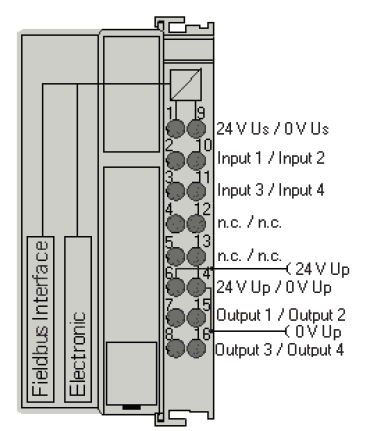
\includegraphics[scale=0.6]{Immagini/Sperimentale/Beckoffschema.PNG}
		\caption{Schema modulo bechoff}
		\label{fig:ModuloBechoff}
	\end{center}
\end{figure}
\subsubsection{Configurazione della rete}
La configurazione della rete prevede alla base il PC Target, in questo vi è una chiavetta USB che fa \textit{runnare} sul pc un sistema operativo simulink real time. Il target è il master della rete, ha due uscite ethernet, la prima è collegata direttamente al modulo bechkoff, il quale prende l'identità di primo slave, e come abbiamo visto precedentemente, al bechkoff sono attaccati e i due azionamenti che si comportano come slave aggiuntivi slave.
\begin{figure}[ht]
\begin{center}
    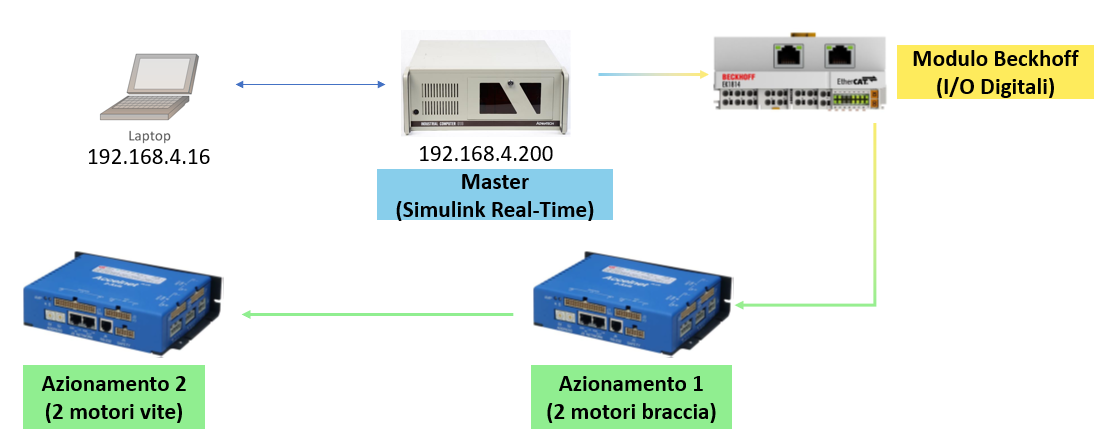
\includegraphics[scale=0.5]{Immagini/Sperimentale/Topology.PNG}
    \caption{Topologia della rete}
    \label{fig:NetTopology1}
\end{center}
\end{figure}
Invece, alla seconda porta ethernet, vi è collegato il PC dell'utente, il quale provvede a generare, compilare, e caricare ed  i programmi sul PC target. Da User-PC è anche possibile vedere i grafici e fare delle analisi sui movimenti e le traiettorie eseguite dal manipolatore. La connessione avviene tramite una rete ethernet, l'indirizzo del target è 192.168.4.200, invece per User-PC:
\begin{figure}[ht]
\begin{center}
    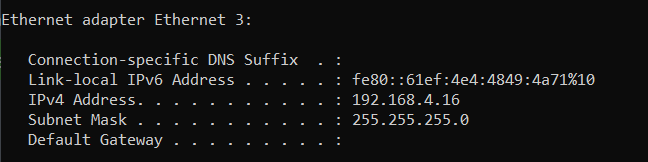
\includegraphics[scale=0.7]{Immagini/Sperimentale/ConfEthernet.png}
    \caption{Configurazione rete ethernet user PC}
    \label{fig:ConfEthernet}
\end{center}
\end{figure}
Va precisato che il pc dell'utente non fa parte della rete ethercat, ma la rete inizia soltanto dal pc target in poi, infatti, ad esclusione delle operazioni viste prima il manipolatore non ha bisogno del pc utente per funzionare.
\begin{figure}[ht]
	\begin{center}
		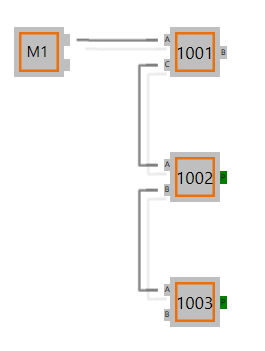
\includegraphics[scale=0.7]{Immagini/Sperimentale/NetTopology.png}
		\caption{Topologia rete mediante Ec-engineer}
		\label{fig:NetTopology2}
	\end{center}
\end{figure}
Una volta configurata la rete, il passo successivo è stato quello della configurazione dei messaggi, come è stato anticipato nel capitolo precedente il metodo di comunicazione sono le PDO. Le PDO possono essere in input o in output, la differenza sta nel fatto che le primo sono PDO che gli azionamenti trasmettono al master, di conseguenza il master le riceve, quelle di output invece sono PDO che il master trasmette e che gli azionamenti ricevono. 
\\Nelle immagini seguenti sono elencate le PDO di input, in particolare:
\begin{itemize}
 	\item PDO1 e PDO2 contengono i parametri di posizione, velocità coppia effettiva e modalità operativa che vengono trasmesse dagli azionamenti
 	\item PDO3, contiene input generici che sono indipendenti dalla modalità operativa del motore, in particolare è presente il \textit{general purpose inputs} che è il registro che permette la visione dei finecorsa
 	\item PDO4 contiene \textit{status word} e \textit{control word}, sono registri importanti che servono per verificare la modalità operativa e lo stato dell'azionamento, quindi sono utili per capire se l'azionamento è in fase pre-operativa, operativa o in errore
\end{itemize}
\begin{figure}[!ht]
\begin{subfigure}{.5\textwidth}
  \centering
  % include first image
  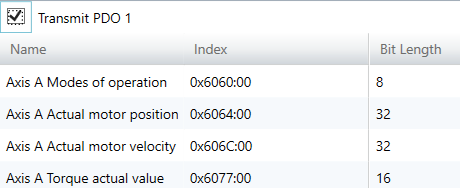
\includegraphics[width=.7\linewidth]{Immagini/Sperimentale/pdo1in.png}  
  \caption{PDO Input 1}
  \label{fig:sub-firstpdo}
\end{subfigure}
\begin{subfigure}{.5\textwidth}
  \centering
  % include second image
  \includegraphics[width=.7\linewidth]{Immagini/Sperimentale/pdo2in.png}  
  \caption{PDO Input 2}
  \label{fig:sub-secondpdo}
\end{subfigure}
\begin{subfigure}{.5\textwidth}
  \centering
  % include third image
  \includegraphics[width=.7\linewidth]{Immagini/Sperimentale/pdo3in.png}  
  \caption{PDO Input 3}
  \label{fig:sub-thirdpdo}
\end{subfigure}
\begin{subfigure}{.5\textwidth}
  \centering
  % include fourth image
  \includegraphics[width=.7\linewidth]{Immagini/Sperimentale/pdo4in.png}  
  \caption{PDO Input 4}
  \label{fig:sub-fourthpdo}
\end{subfigure}
\caption{PDO in input}
\label{fig:PDOIn}
\end{figure}
Per quanto riguarda le PDO che riceve l'azionamento sono solo due, ed i parametri ricevuti sono:
\begin{itemize}
	\item \textit{Modes of operation}, è un registro che specifica la modalità con la verrà controllato l'azionamento, per esempio coppia, posizione, velocità o ciclica
	\item \textit{Target torque}, specifica il valore di coppia che l'azionamento dovrà fornire al motore
\end{itemize}
\begin{figure}[ht]
\begin{center}
    \includegraphics[scale=0.67]{Immagini/Sperimentale/pdo12out.png}
    \caption{PDO Output 1 e 2}
    \label{fig:PDOOut}
\end{center}
\end{figure}
\subsection{Implementazione nel sistema reale}
Una volta ottenuto il file ENI contenente la topologia della rete è stato utilizzato simulink real-time per implementare la logica di controllo del manipolatore
\begin{figure}[ht]
	\begin{center}
		\includegraphics[scale=0.5]{Immagini/Sperimentale/generalSchema}
		\caption{Schema generale simulink}
		\label{fig:SimulinkSchema}
	\end{center}
\end{figure}
Il programma è stato diviso in sei stati diversi, andiamo ad analizzare ora i vari stati.
\subsubsection*{Inizializzazione}
\addcontentsline{toc}{subsubsection}{Inizializzazione}
La prima fase è quella di inizializzazione, in questa fase viene inserito il file ENI e viene specificata la modalità operativa degli azionamenti.
\begin{figure}[ht]
	\begin{center}
		\includegraphics[scale=0.63]{Immagini/Sperimentale/Inizializzazione}
		\caption{Fase 1: Inizializzazione}
		\label{fig:Init}
	\end{center}
\end{figure}
Oltre al file ENI viene anche specificata la porta di comunicazione ed il bus che verranno utilizzati per lo scambio di dati. Ogni azionamento ha poi una determinata modalità operativa, come abbiamo visto nelle sezioni precedenti il controllo è effettuato in coppia. 
\begin{table}[h!]
	\centering
	\begin{tabular}{|c |c|} 
		\hline
		Modalità & Descrizione  \\ 
		\hline
		1 & modalità profilo in posizione  \\ 
		3 & modalità profilo in velocità  \\
		4 & modalità profilo in coppia   \\
		6 & modalità homing \\
		7 & modalità posizione interpolata\\
		\hline
	\end{tabular}
	\caption{Tipologie controllo azionamenti}
	\label{table:5}
\end{table}
\subsubsection*{Input}
\addcontentsline{toc}{subsubsection}{Input}
La seconda fase è quella di input, in questa fase andiamo a prendere tutti i valori di posizione dei motori sia della vite che delle braccia
\begin{figure}[ht]
	\begin{center}
		\includegraphics[scale=0.65]{Immagini/Sperimentale/Input}
		\caption{Fase 2: Input}
		\label{fig:Input}
	\end{center}
\end{figure}
I valori vengono presi mediante i messaggi dalle PDO ed hanno bisogno di essere convertiti, proprio per questo la struttura di ricezione di un messaggio è la seguente: 
\begin{figure}[ht]
	\begin{center}
		\includegraphics[scale=0.7]{Immagini/Sperimentale/convertS}
		\caption{Conversione e lettura motori}
		\label{fig:MotorConversion}
	\end{center}
\end{figure}
\subsubsection*{Stateflow}
\addcontentsline{toc}{subsubsection}{Stateflow}
Lo stateflow è un blocco dove viene posta la logica fondamentale dell'applicazione, in particolare in input avremo tutti i dati come ad esempio il clock, lo stato dei finecorsa, le posizioni dei motori e degli input che serviranno per l'interfaccia grafica. 
\begin{figure}[ht]
	\begin{center}
		\includegraphics[scale=0.65]{Immagini/Sperimentale/sf0}
		\caption{Fase 3: Stateflow}
		\label{fig:Stateflow1}
	\end{center}
\end{figure}
In output invece abbiamo gli offset, che ci serviranno per capire di quanto ci siamo mossi nelle varie fasi, e quindi avere un riferimento sia di posizione che temporale, le coppie di homing dei motori e della vite, e un blocco relativo alla gestione delle luci\footnote{abbiamo la presenza di tre luci: rosso, bianco e verde, nei paragrafi successivi verrà introdotto il loro comportamento}.
\subsubsection*{Controllo vite}
\addcontentsline{toc}{subsubsection}{Controllo vite}
Il blocco Controllo Vite, contiene lo schema del controllore implementato per controllare la vite, in ingresso abbiamo il clock, le posizioni dei motori con relativi offset e la movimentazione da far eseguire ad entrambi i motori della vite con il tempo di esecuzione.
\begin{figure}[ht]
	\begin{center}
		\includegraphics[scale=0.7]{Immagini/Sperimentale/ControlloViteSchema}
		\caption{Fase 4: Schema di controllo della vite}
		\label{fig:ControlloVite}
	\end{center}
\end{figure}
Grazie a tutti questi parametri potremo definire le leggi di moto che ci permetteranno il movimento nell'asse Z. Importante è sapere che il movimento eseguito dalla vite a ricircolo di sfere è dipendente anche dal movimento eseguito dalla guida lineare, infatti la rotazione provoca anche un abbassamento della vite, per risolvere questo problema il motore della guida dovrà essere sempre pronto a rispondere e correggere questa situazione; in caso che i due motori vadano alla stessa velocità si avrà una rotazione senza traslazione.
\subsubsection*{Controllo braccia}
\addcontentsline{toc}{subsubsection}{Controllo braccia}
Il blocco Controllo Braccia è quello responsabile della movimentazione dei link motorizzati, come per il blocco della vite prende in ingresso le posizioni, il \textit{clock} con i relativi offset e dentro vengono svolte le operazioni di generazione della legge di moto e di controllo. In uscita avremo le coppie che saranno assegnate ai due assi.
\begin{figure}[ht]
	\begin{center}
		\includegraphics[scale=0.75]{Immagini/Sperimentale/ControlloBraccia}
		\caption{Fase 5: Schema di controllo delle braccia}
		\label{fig:controlloBraccia}
	\end{center}
\end{figure}
\subsubsection*{Coppie uscita}
\addcontentsline{toc}{subsubsection}{Coppie uscita}
Dopo aver ottenuto le coppie di homing dallo stateflow e le coppie dei motori dagli schemi di controllo è venuto il momento di inviare le coppie agli azionamenti e di conseguenza ai motori; per far questo usiamo un bloco per ogni motore, oltre alle coppie in entrata avremo anche una variabile di controllo. 
\begin{figure}[ht]
	\begin{center}
		\includegraphics[scale=0.55]{Immagini/Sperimentale/Saturatore}
		\caption{Schema espanso invio coppia}
			\label{fig:CoppieoutExpanded}
	\end{center}
\end{figure}
Nella figura precedente è possibile vedere lo schema espanso come spiegato, lo switch permette la scelta in base alla variabile bool, fintanto che è minore o uguale a 3 verrà erogata solo la coppia di Homing, quando arriva a 4 invece vuol dire che siamo nella fase di controllo, di conseguenza verrà erogata la coppia di controllo. Successivo allo switch c'è un blocco che serve per la gestione delle emergenze, infatti, una volta premuto il fungo verrà assegnata una coppia costante uguale a 0 che fermerà la lavorazione ed anche dopo che verrà sbloccato il fungo la coppia per sicurezza rimarrà a zero, l'unico modo per resettare questa condizione è il riavvio del programma.
\begin{figure}[ht]
	\begin{center}
		\includegraphics[scale=0.6]{Immagini/Sperimentale/CoppieOut}
		\caption{Fase 6: Copie in uscita
			\label{fig:Coppieout}}
	\end{center}
\end{figure}
\\Successivo al blocco fungo abbiamo un saturatore, questo serve per evitare di danneggiare il manipolatore in caso che le coppie computate siano molto alte, è stato trovato sperimentalmente un limite che coincide con la coppia nominale che non può essere superato, per concludere l'ultima parte è quella che si occupa di inviare mediante PDO il valore di coppia convertito all'azionamento.
\\Andiamo ora a concentrarci sulle parti principali di questo programma, in particolare andremo a trattare lo stateflow il metodo di funzionamento ed i vari stati, passeremo poi all'interfaccia grafica che permette di comandare il manipolatore, e per concludere andremo a vedere i controllori implementati per la vite e per le braccia, andando a vedere la struttura, lo schema e i risultati ottenuti per ogni approccio.
\subsection{Stateflow}
\textit{Stateflow} si occupa di fornire diagrammi di transizione, stato e di flusso utilizzando un linguaggio grafico. Nel caso del manipolatore è stato utilizzato per la progettazione di diagrammi di transizione in base agli stati del robot. In questa sezione andremo a vedere le fasi gli stadi di evoluzione che sono stati costruiti.
\subsubsection{Fase di Homing}
Appena il robot viene acceso non possiamo sapere dove si trova, di conseguenza abbiamo bisogno di uno stadio che ci vada a trovare una posizione di riferimento nella quale sappiamo dove è collocato effettivamente. Il primo stadio è quindi quello di \textit{homing}, consiste nel portare i motori a toccare i finecorsa indicandogli che quello è il loro punto di partenza. I motori utilizzati per questa fase sono stati quelli delle braccia e quello di traslazione della vite.
\\L'approccio iniziale è stato quello di fornire una coppia costante che in automatico si occupava di andare a toccare i finercorsa, e dopo che li toccava si passava nello stato successivo. Però, per motivi di sicurezza e considerando che lasciando fermo il manipolatore per diverso tempo la stessa coppia magari potrebbe non farlo muovere si è deciso di chiudere l'anello in posizione, in particolare per eseguire la fase di homing è stata data una rampa con pendenza negativa in quanto i finecorsa vengono rilevati quando i link sono totalmente a destra.
Per controllare questa rampa è stato fatto un controllo proporzionale e integrale sull'errore tra la posizione attuale ed il riferimento, la legge implementata è quindi del tipo:
\begin{equation*}
	PI = \frac{K_p s + K_i}{s}
\end{equation*}
Nella figura successiva andiamo a vedere lo schema effettivamente implementato per questa prima fase:
\begin{figure}[ht]
\begin{center}
    \includegraphics[scale=0.8]{Immagini/Sperimentale/state1new.png}
    \caption{Fase di Homing}
    \label{fig:Zero}
\end{center}
\end{figure}
\\Il primo stato è quello di begin, appena il programma si avvia ci entriamo in automatico, per passare allo stato successivo, ovvero attivazione abbiamo bisogno di due condizioni, la prima si verifica quando la \textit{Status Word} è uguale a 1079, ovvero quando gli azionamenti sono usciti dalla fase \textit{pre-operational} e sono quindi pronti all'uso, la seconda condizione invece è quando il segnale avvio è vero, nello stato attivazione i motori sono ancora fermi però viene abilitato il loro utilizzo, passare quindi in questo stato è obbligatorio. Per passare allo stato successivo il segnale \textit{ZeroSignal} deve essere vero, questo è un segnale gestito mediante un bottone da interfaccia grafica, appena viene premuto entriamo nello stato \textbf{Home}. In questo stato vengono definite variabili per la conversione dei valori\footnote{I valori presi dai motori sono espressi tutti in conti, per quello è stata necessaria una fase di analisi dei motori per capire come convertirli, successivamente c'è stato un passaggio da counts a radianti e da radianti a gradi.}, viene poi salvata la posizione di riferimento dell'asse A e B dei motori delle braccia. La fase successiva è quella del \textit{during}, rimanendo in quello stato quella fase viene eseguita ad ogni ciclo (1ms), in questa abbiamo la rampa che decresce di 0.015 gradi al millisecondo (15 gradi al secondo) e abbiamo una funzione simulink che è quella che si occupa del controllo PI. Una volta raggiunta la posizione del finecorsa le coppie vengono settate a 0, impedendo quindi un'ulteriore movimentazione. Per passare alla fase successiva abbiamo bisogno che tutti gli elementi siano arrivati a finecorsa.
\subsubsection{Fase di posizionamento}
La fase successiva è quella di posizionamento, per non lasciare il robot nella configurazione di zero si è scelto di spostarlo in una configurazione standard lontana dai punti di singolarità e che sarà comoda per le movimentazioni e traiettorie successive. La configurazione scelta prevede che i giunti siano messi a $100^\circ$ e $80^\circ$, anche qua come prima il primo approccio è stato quello di utilizzare una coppia costante per il movimento; la fase di zero lasciava i link a $60^\circ$ e $-30^\circ$, vi era quindi la necessità di fare $+40^\circ$ per il motore a sinistra e $+110^\circ$ per il motore a destra, la coppia costante veniva erogata finché non si arrivava a quelle condizioni, dopodiché eravamo sicuri che il posizionamento era stato fatto in maniera corretta. La vite invece ha due modalità di configurazione, è possibile farla abbassare o lasciarla alta in finecorsa, si è scelto di proseguire in questo modo in quanto alla vite come abbiamo visto precedentemente è possibile collegare degli utensili e quindi l'abbassamento la predisponeva al disegno per traiettorie bidimensionali. L'approccio di controllo finale però non è stato quello della coppia costante, anche in questo caso per motivi di sicurezza ma, sapendo le posizioni finali che si volevano raggiungere, si è optato per definire una legge di moto che si occupava di portarci in quella condizione.
\begin{figure}[ht]
\begin{center}
    \includegraphics[scale=0.31]{Immagini/Sperimentale/state2.png}
    \caption{DA CAMBIARE}
    \label{fig:Pos}
\end{center}
\end{figure}
\\Inserisci descrizione schema
\subsubsection{Fase di controllo}
L'ultima fase è quella di controllo ed esecuzione della traiettoria, in questa fase andiamo a settare l'offset dei motori della vite, del tempo e dei motori delle braccia, serve resettare l'offset della vita in quanto il posizionamento (nel caso di discesa) è stato appena concluso; l'offset del tempo ci permette di far partire virtualmente il tempo da zero negli schemi di controllo dopo che siamo arrivati alla configurazione di \textit{Homing}.
\begin{figure}[ht]
\begin{center}
    \includegraphics[scale=0.6]{Immagini/Sperimentale/state3New.png}
    \caption{Fase di controllo}
    \label{fig:Traiettoria}
\end{center}
\end{figure}
Come abbiamo anticipato precedentemente nello stato \textbf{OffSet} c'è il settaggio degli \textit{offset} e tutte le coppie vengono messe a zero per evitare eventuali movimentazioni indesiderate. Per passare alla fase successiva abbiamo bisogno che venga premuto il bottone \textbf{Work} sull'interfaccia grafica, questo garantirà il passaggio allo stato \textit{Controllo}, può darsi che il bottone non venga premuto subito, di conseguenza il clock potrebbe aumentare, per questo l'offset del clock viene settato nella fase di controllo. Per quanto riguarda la scelta della traiettoria tramite interfaccia grafica vi è la possibilità di scegliere quella desiderata. A livello implementativo le traiettorie non sono altro che leggi di moto fatte in due o tre dimensioni, dipendentemente dal caso, dopo che il manipolatore inizia ad eseguire la traiettoria possono esserci due evoluzioni:
\begin{itemize}
	\item la traiettoria viene eseguita correttamente
	\item la traiettoria da problemi
\end{itemize}
Nel primo caso abbiamo 40 secondi per eseguire la traiettoria (il tempo può essere personalizzato in base alla tipologia di traiettorie), alla fine di questo tempo passiamo allo stato \textbf{FineLavorazione} dove il manipolatore è fermo ed ha concluso la sua traiettoria, da questo mediante il bottone di reset è possibile ritornare alla fase di zero, oppure in automatico dopo un determinato periodo di tempo se il tasto di homing è stato lasciato attivo il manipolatore torna all'homing. Nel secondo caso ci si accorge che la traiettoria sta dando problemi, magari vibrazioni o si vede che il manipolatore rischia di entrare in singolarità, per prevenire questo vi è un bottone denominato \textbf{STOP} che permette l'arresto immediato del manipolatore, azzerando tutte le coppie. A differenza della pressione del fungo, che dopo lo sbloccaggio richiede il riavvio del dispositivo, nel caso in cui si entri nella fase di stop mediante il bottone di reset è possibile far tornare il manipolatore nella fase di attivazione, da questa poi sarà possibile far partire di nuovo la fase di zero e successivamente quella di homing.

\subsubsection*{Gestione variabile di stato e luci}
\addcontentsline{toc}{subsubsection}{Gestione variabile di stato e luci}
Durante tutte le fasi è possibile vedere nello stateflow che due variabili si evolvono costantemente: bool e luci; la prima serve per indicare lo stato nel quale si trova il manipolatore, in particolare è state definita la seguente tabella degli stati.
\begin{table}[h!]
\centering
\begin{tabular}{|c |c |} 
 \hline
 Valore & Stato \\ [0.5ex] 
 \hline\hline
  -1  & Pre-operativo \\ 
  0  & Attivo \\
  1 & Homing \\
  2 & Manipolatore posizionato\\
  3 & Traiettoria\\
  4 & Manipolatore fermo\\
 \hline
\end{tabular}
\caption{Valori variabile \textit{bool}}
\label{table:3}
\end{table}
\\La seconda invece serve a pilotare le luci in modo tale da avere un feedback visuale che indica fase in cui è il manipolatore.
\begin{table}[h!]
\centering
\begin{tabular}{|c |c|c|} 
 \hline
 Valore & Colore & Bool \\ [0.5ex] 
 \hline\hline
  1  & Bianco & 1 \\ 
  2 &  Bianco Rosso & 1\\
  3 &  Rosso & 2 \\
  4 & Bianco Verde & 3\\
  5 & Verde & 4\\
 \hline
\end{tabular}
\caption{Valori luci}
\label{table:luci}
\end{table}
\subsubsection{Interfaccia grafica}
Per gestire al meglio le varie impostazioni, e per essere sicuri del passaggio tra i vari stati è stata creata un'interfaccia grafica \textit{user-friendly} mediante \textit{instrument panel} fornito da \textit{Simulink real-time explorer}
\begin{figure}[ht]
	\begin{center}
		\includegraphics[scale=0.49]{Immagini/Sperimentale/GUI2}
		\caption{Interfaccia grafica}
		\label{fig:gui}
	\end{center}
\end{figure}
\\A sinistra, dall'alto in basso possiamo vedere dei LED che hanno la funzionalità di:
\begin{itemize}
	\item Fungo: rimane acceso fintantoché il fungo non è premuto
	\item Homing: si accendono quando i motori hanno raggiunto il finecorsa
	\item Fine lavoro: appena la traiettoria assegnata finisce questo si accende
	\item Luci: sono i led visti nella tabella \ref{table:luci}, che vanno ad indicare in che fase di lavoro è il manipolatore, per comodità visiva il led bianco nell'interfaccia è stato sostituito da uno ocra
\end{itemize} 
Sotto questi led abbiamo un indicatore che va a specificare le fasi di lavoro come viste nella tabella \ref{table:3}. Al centro abbiamo i bottoni che permettono di passare tra le varie fasi dello stateflow e di fare tutte le operazioni quindi avvio, zero, homing, lavoro stop e reset. In particolare i bottoni funzionano tramite il collegamento ad una variabile, e quelle di riferimento sono le ultime costanti collegate in input allo stateflow visto in figura \ref{fig:Stateflow1}. A destra abbiamo invece una parte di visualizzazione dove vediamo tutti i parametri di interesse del manipolatore, in particolare le coppie fornite e le posizioni sia nel piano $[x,y,z]$ che quelle ai link motorizzati quindi $\theta_1,\theta_2$. Infine, abbiamo il selettore di traiettoria, il quale permette la scelta fra le sei opzioni possibili (di default viene eseguito il cerchio).
\begin{enumerate}
	\item Quadrato
	\item Cerchio
	\item Pattern
	\item Cerchi tangenti
	\item Spirale
	\item Solo asse Z
\end{enumerate}
Adesso che abbiamo introdotto la logica di funzionamento a stati, proseguiamo la nostra trattazione andando a vedere le tipologie di controllo che sono state implementate, in particolare inizieremo col guardare il controllo applicato alla vite e successivamente quello per le braccia.
\subsection{Controllo vite}

\subsubsection{Controllo proporzionale}
\subsubsection{Controllo proporzionale derivativo}
\subsection{Controllo braccia}
Questa sottosezione si pone come obiettivo l'introduzione di approcci di controllo noti in letteratura e applicarli ai link motorizzati del manipolatore; in particolare andando ad analizzare il loro funzionamento a livello teorico, la loro implementazione pratica ed i risultati ottenuti, cercando quindi il controllore migliore. Tutte le tipologie di controllo introdotte saranno di tipo centralizzato, gli algoritmi di questa tipologia sfruttano una conoscenza più approfondita del modello dinamica del manipolatore in modo tale da compensare i termini di accoppiamento non lineari, verranno quindi introdotte coppie di compensazione per i termini NL, inoltre, qualsiasi incertezza della struttura e qualunque imprecisione nella misura della posizione daranno origine ad una perdita di accuratezza e quindi a problemi di controllo.
\subsubsection{Controllo proporzionale derivativo}
La prima tipologia di controllo applicata è stata quella proporzionale derivativa. L'obiettivo di questa tecnica è quello di risolvere il problema della regolazione, ovvero assegnare la posizione corretta all'end-effector rispetto ad un riferimento di equilibrio costante. Non viene risolto il problema della dinamica con la quale si raggiunge quella configurazione, però come obiettivo ci si pone di trovare la struttura del controllore che ci assicuri una stabilità asintotica in quella specifica posa desiderata. Definiamo lo stato come: 
\begin{equation}
\tilde{q} = q^0_m - q_m
\end{equation}
Con $q^0_m$ che rappresenta il \textit{set-point} (posizione desiderata) e $q_m$ la posizione attuale, per poter andare a risolvere il problema abbiamo bisogno di introdurre il metodo diretto di Lyapunov, il quale dice che: 
\begin{center}
\textit{L’analisi della stabilità di un punto di equilibrio viene fatta utilizzando, oltre alle equazioni di stato del sistema, opportune funzioni scalari, dette funzioni di Lyapunov, definite sullo spazio degli stati. }
\end{center}
Definiamo quindi la funzione come:
\begin{equation}
V(\dot{q:m},\tilde{q}) = \frac{1}{2} \dot{q_m}M(q_m)\dot{q_m} + \frac{1}{2} \tilde{q}K_p \tilde{q} >0
\end{equation}
Il termine $K_p$ rappresenta la rigidezza del sistema ed è una matrice $(n x n)$ simmetrica e definita positiva. Considerando che il \textit{set-point} è un termine costante possiamo  andare a derivare la funzione V rispetto al tempo ottenendo:
\begin{equation*}
\dot{V} = \ddot{q_m}M(q_m)\dot{q_m}+\frac{1}{2} \dot{q_m}\dot{M}(q_m)\dot{q_m}-\dot{q_m}K_p\tilde{q}
\end{equation*}
e sapendo che $\tau_m = M(q_m)\ddot{q_m} + C(q_m,\dot{q_m)})\dot{q_m}$\footnote{Nella trattazione di Lyapunov appare anche il termine di compensazione gravitazionale però nel manipolatore analizzato questo termine è costante e pari a zero.} possiamo riscrivere la funzione come 
\begin{equation}
\dot{V} = \dot{q_m} [\tau_m - K_p \tilde{q}]
\label{eq:finLap}
\end{equation}
Se adesso consideriamo la legge di controllo PD definita come:
\begin{equation}
\tau_m = K_p\tilde{q} - K_d\dot{q_m}
\end{equation}
e andiamo a sostituirla nell'equazione \ref{eq:finLap} otteniamo
\begin{equation*}
\dot{V} = -\dot{q_m}K_d \dot{q_m} \le 0
\end{equation*}
Se $K_d$ è una matrice definita positiva allora $\dot{V}$ è semidefinita negativa, la dinamica del sistema è quindi:
\begin{equation}
M(q_m)\ddot{q_m} + C(q_m,\dot{q_m})\dot{q_m} = K_p\tilde{q}-K_d\dot{q_m}
\end{equation}
In particolare abbiamo che velocità ed accelerazioni sono nulla in corrispondenza di $\dot{V} = 0$. Possiamo andare ora a vedere lo schema di controllo:
INSERISCI PARTE PRATICA
\subsubsection{Controllo feed-forward con coppia pre-computata}
Il passo successivo è stato quello di studiare ed implementare un controllore che opera in anello aperto; in particolare questo controllore calcola le coppie di disturbo basate sul modello matematico del sistema con parametri d'ingresso il \textit{set-point} in posizione e velocità e accelerazione. L'introduzione di questi termini riesce a risolvere in maniera corretta il problema del tracciamento della traiettoria desiderata, di conseguenza gli elementi introdotti riescono a compensare gli effetti di accoppiamento presenti nel modello dinamico del sistema. 
\begin{equation}
g_d = \Delta M(q^0_m)\ddot{q_m}^0 + C(q^0_m,\dot{q_m^0})\dot{q_m^0}
\end{equation}
L'idea è quindi che i termini vengono calcolati considerando i valori di posizione, velocità ed accelerazione del rifermento, in quanto mediante una legge di moto sono sempre ben noti. L'elemento $g_d$ compensa i termini di accoppiamento non lineari dovuti a forza d'inerzia, di Coriolis e centrifughe che dipendono dalla struttura e di conseguenza variano durante il movimento del manipolatore; in generale però calcolare questo termine è molto impegnativo, di conseguenza l'utilizzo di questo approccio su un sistema online può richiedere molto tempo, per questo solitamente vengono compensati solo i termini più importanti come quelli inerziali.
INSERISCI SCHEMA ETC
\subsubsection{Controllo in dinamica inversa}
Riprendendo le tecniche di controllo centralizzato caratteristiche della letteratura l'approccio successivo è stato quello del controllo in dinamica inversa. Il primo step è stato quello di prendere l'equazione della dinamica e ridefinirla come: 
\begin{equation}
M(q_m)\ddot{q_m} + n(q_m,\dot{q_m}) = \tau_m
\label{eq:ControlloreID}
\end{equation}
Dove $n(q_m,\dot{q_m})$ raccoglie i termini centrifughi e di Coriolis (in letteratura raccoglie anche i termini gravitazionali, ma come anticipato precedentemente nel nostro caso equivalgono a zero). L'idea del controllo a dinamica inversa si basa sul trovare il vettore di coppie $\tau_m$ come funzione dello stato del sistema, cercando di creare una relazione ingresso-uscita di tipo lineare. Considerando che l'equazione della dinamica è lineare nel controllo e che la matrice d'inerzia è invertibile in ogni configurazione del manipolatore abbiamo la garanzia di trovare un controllore linearizzato di questo tipo. Possiamo andare a riscrivere il controllo come:
\begin{equation}
\tau_m = M(q_m)y + n(q_m,\dot{q_m})
\end{equation}
Dove $y = \ddot{q_m}$ rappresenta un vettore d'ingresso con espressione ancora da determinare. La legge di controllo è basata sul calcolo della dinamica inversa del manipolatore, il sistema è lineare e disaccoppiato rispetto al nuovo ingresso, questo implica che le componenti $y_k$ con $k = -\infty \dots m-1$ influenzano solo la variabile $q_m$ indipendentemente dal movimento degli altri giunti. In questo modo il problema del controllo è quello di trovare una legge \textbf{y} stabilizzante. Viene quindi scelta:
\begin{equation}
y = K_p\tilde{q} + K_d\tilde{\dot{q}}+\ddot{q}_m^0
\label{eq:yID}
\end{equation}
Dove con i termini $\tilde{q}$ e $\tilde{\dot{q}}$ si indica la differenza tra il \textit{setpoint} e la misurazione attuale di posizione e velocità. 
\begin{equation}
\tilde{q} = q^0_m - q_m \ \ \  \tilde{\dot{q}}= \dot{q}^0_m-\dot{q}_m
\label{eq:Tilde}
\end{equation}
Possiamo andare ora a sostituire le definizioni di \ref{eq:Tilde} in \ref{eq:yID} e troviamo l'espressione:
\begin{equation}
\tilde{\ddot{q}} + K_d + \tilde{\dot{q}} = 0
\end{equation}
Chiaramente l'errore si verifica quando uno o entrambi i termini sono diversi da zero.  Però, volendo assegnare la dinamica a ciascun giunto ci basta selezionare  i guadagni delle matrici $K_p$ e $K_d$ , inoltre, se le due matrici sono definite positive è possibile ottenere un sistema asintoticamente stabile. 
Possiamo scegliere le matrici come:
\begin{equation*}
K_p = diag(\omega^2_{01}, \dots, \omega^2_{0n}) \overline{M} \ \ \  K_d = diag(2 \xi_1 \omega_{01}, \dots ,2 \xi_n \omega_{0n}) \overline{M} 
\end{equation*}
Grazie al controllo a dinamica inversa i termini di compensazioni vengono calcolati ad ogni iterazione, quindi a piccoli intervalli temporali, il loop interno serve per ottenere una relazione ingresso/uscita lineare e disaccoppiata mentre quello esterno grazie alla dinamica desiderata serve a stabilizzare il sistema.
INSERISCI SCHEMA
\par L'utilizzo di questo approccio è basato sull'ipotesi della cancellazione perfetta dei termini dinamici, quindi, i parametri dinamici del sistema devono essere accuratamente conosciuti e l'equazione del moto deve essere calcolata in real-time.
\subsubsection*{Implementazione controllore}
\addcontentsline{toc}{subsubsection}{Implementazione controllore}
\subsubsection*{Test Kp e Kd}
\addcontentsline{toc}{subsubsection}{Test Kp e Kd}
L'approccio successivo è stato quello di continuare con la dinamica inversa ma chiudendo l'anello, [inserisci schema]
Un test che è stato fatto per andare a ricercare i parametri è stato quello di far variare $K_p$, in un range di valori compreso tra 350 e 950 ad intervalli di 50, in base ad un valore fisso di $K_d$, andiamo ora a vedere un risultato di questo metodo.
\begin{figure}[!ht]
\begin{subfigure}{.5\textwidth}
  \centering
  % include first image
  \includegraphics[width=.8\linewidth]{Immagini/Sperimentale/Test_Kd=15.png}  
  \caption{Test con $K_d$ = 1.5}
  \label{fig:sub-kd1.5}
\end{subfigure}
\begin{subfigure}{.5\textwidth}
  \centering
  % include second image
  \includegraphics[width=.8\linewidth]{Immagini/Sperimentale/Test_Kd=2.png}  
  \caption{Test con $K_d$=2}
  \label{fig:sub-kd2}
\end{subfigure}
\begin{subfigure}{.5\textwidth}
  \centering
  % include third image
  \includegraphics[width=.8\linewidth]{Immagini/Sperimentale/Test_Kd=3.png}  
  \caption{Test con $K_d$=3}
  \label{fig:sub-kd3}
\end{subfigure}
\begin{subfigure}{.5\textwidth}
  \centering
  % include third image
  \includegraphics[width=.8\linewidth]{Immagini/Sperimentale/Test_Kd=3.png}  
  \caption{Test con $K_d$=3}
  \label{fig:sub-kd1}
\end{subfigure}
\caption{Test su $K_d$}
\label{fig:KdTest}
\end{figure}
Si può chiaramente vedere come all'aumentare di $K_d$ i valori di $K_p$ iniziano ad vibrare sempre prima. Come valori finali per questo controllore sono stati scelti $K_d = \frac{3}{2}$ e $K_p = 720$
\subsubsection*{Traiettorie testate}
\addcontentsline{toc}{subsubsection}{Traiettorie testate}
\subsubsection{Controllo robusto}
 L'effetto di incertezze sul modello induce in errore il sistema di controllo, soprattutto nel caso reale bisogna supporre che la compensazione del modello dinamico risulti imperfetta magari a causa di approssimazioni oppure per semplificazioni.  Possiamo andare quindi a riscrivere l'equazione \ref{eq:ControlloreID} come:
\begin{equation}
\tau_m = \hat{M}(q_m)y + \hat{n}(q_m,\dot{q}_m)
\end{equation}
Dove $\hat{M}$ e $\hat{n}$ rappresentano i parametri stimati del modello dinamico, è possibile rappresentare l'incertezza come:
\begin{equation*}
\overline{M} = \hat{M}- M \ \ \overline{n} = \hat{n} - n
\end{equation*}  
Riprendendo la legge di controllo vista prima possiamo riscriverla come:
\begin{equation}
M(q_m)\ddot{q}_m + n(q_m,\dot{q_m}) = \hat{M}(q_m)y + \hat{n}(q_m,\dot{q_m})
\end{equation}
Essendo la matrice M invertibile in ogni configurazione possiamo ricavare $\ddot{q}_m$:
\begin{equation*}
\ddot{q}_m = y + (M^{-1}\hat{M}-I)y+M^{-1}\tilde{n} = y-\eta
\end{equation*}
Dove $\eta$ è una funzione non lineare definita come: \begin{equation}
\eta = (I-M^{-1}\hat{M})y - M^{-1}\tilde{n} 
\end{equation}
Adottando la legge \ref{eq:Tilde} vista nel caso del controllore a dinamica inversa possiamo ottenere che l'errore dinamico è gestito dall'equazione:
\begin{equation}
\ddot{\tilde{q}} + K_d \dot{\tilde{q}} + K_p\tilde{q} = \eta
\end{equation}
Otteniamo quindi un sistema non lineare e accoppiato, di conseguenza implementare un semplice controllore PD non basta; per risolvere questo problema occorre inserire un termine non lineare, che sia funzione dell'errore e creato appositamente per fornire robustezza al controllo. Come per il controllore PD si ricerca una funzione grazie al metodo diretto di Lyapunov. 
Andiamo a definire lo stato del sistema come:
\begin{equation*}
\xi = \begin{bmatrix}
\tilde{q} \\ \dot{\tilde{q}}
\end{bmatrix}
\end{equation*}
sostituendo poi lo stato nell'equazione $\ddot{q}_m = y-\eta$ si ottiene un'equazione differenziale del primo ordine
\begin{equation}
\dot{\xi} = H\xi + D(\ddot{q}_m^0 - y + \eta)
\end{equation}
Dove H e D sono definite come:$H = \begin{bmatrix}
0 & I \\ 0 & 0
\end{bmatrix} \in \mathbb{R}^{(2nx2n)}$ , $D = \begin{bmatrix}
0 \\ I
\end{bmatrix} \in \mathbb{R}^{(2nxn)}$
\\Si può vedere il problema di inseguimento della traiettoria come la soluzione che va a stabilizzare il sistema non lineare di qui sopra. Nella letteratura del controllore robusto, anche se l'incertezza $\eta$ non è nota è comunque disponibile un suo intervallo di variazione. La legge \textbf{y} dovrebbe garantire stabilità di $\dot{\xi}$ per ogni $\eta$ nell'intervallo. Di conseguenza vengono formulate tre assunzioni:
\begin{enumerate}
\item $\sup_{t\ge 0} ||\ddot{q}^0_m || < Q_M < \infty \forall \ddot{q}_m^0$
\item $||I-M^{-1}\hat{M}(q_m)|| \le \alpha \le 1 \forall q_m$
\item $||\tilde{n}|| \le \Phi(||\xi||) < \infty \forall q_m, \dot{q}_m$
\end{enumerate}
Andando ad analizzare le assunzioni possiamo dire che:
\begin{itemize}
\item La prima assunzione è soddisfatta sempre, in quanto per ogni traiettoria definita le accelerazioni non possono essere infinite
\item La seconda assunzione conferma che M  (e di conseguenza $M^{-1}$) sia superiormente e inferiormente limitata, infatti 
\begin{equation}
0 < M_m < ||M^{-1}(q_m)|| \le M_M < \infty \forall q_m
\end{equation}
\end{itemize}
Quindi, esiste sempre una scelta di $\hat{M}$ che soddisfa la condizione, selezionando per esempio
\begin{equation*}
\hat{M} = \frac{2}{M_M+M_m}I
\end{equation*} 
otteniamo
\begin{equation}
||M^{-1}(q_m)\hat{M}(q_m)-I|\le \alpha = \frac{M_M-M_m}{M_M+M_m} <1
\end{equation}
Il limite inferiore si ha quando $\hat{M} = M$ in quanto $\alpha = 0$. Concentrandoci sull'assunzione 3, si può osservare che $\tilde{n}$ è funzione di $q_m,\dot{q_m}$, nel primo caso, in base alla tipologia di giunto (rotoidale o prismatico) abbiamo intervalli che sono limitati e quindi il contributo è limitato. Anche la velocità è limitata grazie all'effetto della saturazione (esistente sulle velocità massime dei motori). Di conseguenza, prendiamo per $\Phi$ una funzione calcolata nella norma dello stato come:
\begin{equation}
\Phi(||\xi||) = \alpha_0 + \alpha_1 ||\xi|| + \alpha_2 ||\xi||^2
\end{equation}
Andando a riprendere la legge di controllo\ref{eq:yID} ed ampliandola possiamo definirla come: 
\begin{equation}
y = \ddot{q}^0_m + K_p\tilde{q} + K_d\dot{\tilde{q}} + \omega
\label{eq:yRob}
\end{equation}
Il termine PD ci assicura la stabilizzazione della dinamica della matrice dell'errore, $\ddot{q}^0_m$ fornisce un termine di previsione e $\omega$ è progettato in modo da combattere l'incertezza fornendo robustezza al sistema.
\begin{equation}
\dot{\xi} = \tilde{H}\xi + D(\eta-\omega)
\end{equation}
Dove:
\begin{equation*}
\tilde{H} = H-DK = \begin{bmatrix}
0 & I \\ -K_p & -K_d
\end{bmatrix} \in 
\mathbb{R}^{(2nx2n)}
\end{equation*}
\begin{equation*}
 \ K_p = diag(\omega^2_{01}, \dots, \omega^2_{0n})  \ \ \  K_d = diag(2 \xi_1 \omega^2_{01}, \dots ,2 \xi_n \omega^2_{0n}) 
\end{equation*}
Per andare a definire $omega$ si procede col metodo diretto di Lyapunov; consideriamo come funzione:
\begin{equation}
V(\xi) = \xi^TQ\xi >0 , \forall \xi \neq 0
\end{equation}
con Q matrice simmetrica definita positiva. Facendo la derivata lungo la traiettoria si trova che
\begin{equation}
\dot{V} = \xi^T P\xi + 2z^T(\eta-\omega)
\label{eq:LyapDerivRob}
\end{equation}
Considerando che $\tilde{H}$ ha tutti gli autovalori con parte reale negativa, possiamo scegliere una qualunque P definita positiva che soddisfi:
\begin{equation*}
\tilde{H}^TQ+Q\tilde{H} = -P
\end{equation*}
Consideriamo ora l'equazione \ref{eq:LyapDerivRob} , $z = D^TQ\xi$, il primo termine sulla parte di destra è definito negativo, di conseguenza la soluzione converge solo se $\xi \in \mathbb{N}(D^TQ)$, se invece non appartiene, il controllo $\omega$ andrà scelto per rendere il secondo termine minore o uguale a zero utilizzando la legge di controllo:
\begin{equation}
\omega = \rho(||\xi||)\frac{z}{||z||}, \rho >0
\end{equation}
con $\rho$ funzione positiva da determinare. Scegliendo $\omega$ in questo modo otteniamo:
\begin{equation*}
z^T(\eta-\omega) = z^T\eta - \rho(||\xi||)\frac{zz^T}{||z||} \le ||z||\big[||\eta||.\rho(||\xi||)\big]
\end{equation*}
se poi garantiamo che: $||\xi||>||\eta||$ per ogni valore di posizione, velocità e velocità di riferimento, otteniamo che questo termine e $\dot{V}$ sono negativi lungo tutte le traiettorie dell'errore; per poter soddisfare la disuguaglianza, dalla definizione di $\eta$ troviamo:
\begin{equation}
\eta = (I-M^{-1}\hat{M})y-M^{-1}\tilde{n} \ e \ y = \ddot{q}^0_m + K\xi+\omega
\end{equation}
sapendo poi che $||\omega|| = \rho$ troviamo che:
\begin{equation*}
||\eta|| \le ||I-M^{-1}\hat{M}|| (||\ddot{q}_m^0 ||+||K||\  ||\xi||+||\omega||)+||M^{-1}|| \ ||\tilde{n}||
\end{equation*}
Andando a maggiorare questa quantità troviamo che:
\begin{equation}
||\eta|| \le \alpha Q_M + \alpha ||K|| || \xi || + \alpha\rho(||\xi||)+M_M\Phi(||\xi||) < \rho(||\xi||)
\end{equation}
è quindi possibile andare a selezionare un $rho$ in modo tale che:
\begin{equation}
\rho(||\xi||) \ge \frac{1}{1-\alpha} [\alpha Q_M+\alpha ||K|| ||\xi||+M_M\Phi(||\xi||)]
\label{eq:HelpRho}
\end{equation}
Si può osservare che $\Phi(||\xi||) = \alpha_0+\alpha_1||\xi||+\alpha_2||\xi||^2$ per soddisfare \ref{eq:HelpRho} basta che si selezionino:
\begin{equation*}
\rho(||\xi||) = \beta_0 + \beta_1||\xi||+\beta_2||\xi||^2
\end{equation*}
Con i valori:
\begin{equation*}
\begin{cases}
\beta_0 \ge \frac{\alpha Q_M+\alpha_0M_M}{1-\alpha}\\
 \beta_1 \ge \frac{\alpha K +\alpha_1 M_M}{1-\alpha}\\
 \beta_2 \ge \frac{\alpha_2M_M}{1-\alpha}
\end{cases}
\end{equation*}
Andando poi a sostituire tutto nell'equazione \ref{eq:LyapDerivRob} troviamo:
\begin{equation}
\dot{V} = -\xi^T P \xi + 2z^T(\eta-\rho(||\xi||) \frac{z}{||z||}) <0 \ \forall
\xi \neq 0
\end{equation}
Di conseguenza $\xi = 0$ è un equilibrio di stato asintoticamente e globalmente stabile. La legge di controllo è quindi formata da tre termini, un primo termine che compensa i termini non lineari e gli accoppiamenti tra i link, un secondo terine che stabilizza il sistema dinamico grazie ad una retroazione con previsione per l'errore e un terzo termine che fornisce robustezza contrastando le incertezze e calcolando i termini non lineari che dipendono dallo stato del manipolatore. 
\par Ad alte frequenze però potrebbe esserci la commutazione della variabile di controllo, che potrebbe portare ad un'elevata presenza di "sali/scendi" a causa del terzo termine, per questo possiamo approssimarlo come:
\begin{equation}
\omega = \begin{cases}
\rho(||\xi||) \frac{z}{||z||} \ for\ ||z||\ge \varepsilon \\
\rho(||\xi||) \frac{z}{\varepsilon} \ \ \ for \ ||z|| < \varepsilon
\end{cases}
\end{equation}
\\INSERISCI SCHEMA ETC
\subsubsection*{1 gdl}
\addcontentsline{toc}{subsubsection}{1 gdl}
\subsubsection*{tt}
\addcontentsline{toc}{subsubsection}{tt}
\subsection{Traiettorie eseguite}
In questa sezione andremo a vedere ed analizzare tutte le traiettorie che sono state create, le traiettorie variano da bidimensionali a tridimensionali, andando anche ad includere due pattern.


\section{Conclusioni}
L'obiettivo principale della tesi è stato lo studio e l'analisi di approcci di controllo centralizzato al fine di trovare quello migliore da implementare nel manipolatore.
\\Dopo la trattazione sulla cinematica, dinamica e cinetostatica del sistema è stato possibile definire le relazioni matematiche che caratterizzano le due parti del manipolatore, braccia e vite, il workspace ed i possibili punti raggiungibili ed implementare quanto visto su un modello simulato. Il modello una volta validato grazie a processi di cosimulazione (Matlab e Adams) ha fornito una base per l'implementazione degli schemi di controllo.
\par L'implementazione di differenti tecniche ha permesso di ottenere una maggior conoscenza nell'ambito della manipolazione del 5R e la fase di simulazione ha permesso di definire quale tra le strategie analizzate fosse la più consona, andando a scartare l'impiego di altri criteri; uno in particolare è stato il controllo robusto, influenzato da fenomeni vibratori generati dalla commutazione ad alta frequenza della variabile di controllo.
\par Per concludere, la validazione sperimentale ha permesso di evidenziare che il criterio ottimo di controllo è quello a dinamica inversa, in quanto con questa tipologia si riesce ad ottenere un \textit{trade-off} tra prestazioni e  robustezza. L'ultima fase è stata quella di test, andando ad implementare traiettorie bidimensionali e tridimensionali ed analizzare come il controllo andava a comportarsi.
\subsection*{Sviluppi futuri}
\addcontentsline{toc}{subsection}{Sviluppi futuri}
Gli obiettivi futuri legati al progetto di tesi riguardano nuovi criteri di controllo, andando ad analizzare tipologie di controllo diverse che potrebbero essere implementate ed dare risultati migliori di quella dinamica inversa. Un'altra tematica riguarda il telecontrollo del manipolatore, che assumerà il ruolo di slave, da un'interfaccia aptica con sensore di forza.


\newpage
\thispagestyle{plain} % empty
\mbox{}
\begin{appendices}
\section{Formule estese}
In riferimento al capitolo della cinematica e della dinamica andiamo ora a vedere le formule per esteso:
\subsection{Formule cinematica diretta accelerazione}
Andiamo a concentrarci sulle formule viste nel capitolo della cinematica diretta di accelerazione. [metti riferimento]
\begin{equation}
\dot{J}_{11} = A_{11} - B_{11} - C_{11} - D_{11}
\end{equation}
Andiamo ora a definire i parametri: 
\begin{equation*}
A_{11} = \frac{l(y-l\sin\theta_{2})(d\sin\theta_{1}-y\cos\theta _{1}+x\sin\theta _{1})\cdot (\dot{y}-l\dot{\theta_1}\cos\theta _{1}+A_{1.1.2})}{(d-x+l\cos\theta_{2})(y-l\sin\theta_{1}+\frac{(y-l\sin\theta _{2})(d+x-l\cos\theta _{1})}{d-x+l\cos\theta _{2}})^2}
\end{equation*}
\begin{equation*}
\begin{split}
A_{1.1.2} = \frac{(y-l\sin\theta_{2})(\dot{x}+l\dot{\theta_1}\sin\theta_{1})}{d-x+l\cos\theta_{2}}+\frac{\dot{y}-l\dot{\theta_2}\cos\theta_{2}(d+x-l\cos\theta_{1})}{d-x+l\cos\theta_{2}}+  \\
+ \frac{(y-l\sin\theta_{2})(\dot{x}+l\dot{\theta}_{2}\sin\theta_{2})(d+x-l\cos\theta_{1})}{{(d-x+l\cos\theta_{2})}^2}
\end{split}
\end{equation*}
\begin{equation*}
B_{11} =\frac{l(y-l\sin\theta_{2})(\dot{x}\sin\theta_{1}-\dot{y}\cos\theta_{1}+d\dot{\theta_1}\cos\theta_{1}+\dot{\theta_1}x\cos\theta_{1}+\dot{\theta_{1}}y\sin\theta _{1})}{(d-x+l\cos\theta_{2})\cdot(y-l\sin\theta_{1}+\frac{(y-l\sin\theta_{2})(d+x-l\cos\theta_{1})}{d-x+l\cos\theta_{2}})}
\end{equation*}
\begin{equation*}
C_{11} = \frac{l(\dot{y}-l\dot{\theta_{2}}\cos\theta_{2})(d\sin\theta_{1}
    -y\cos\theta_{1}+x\sin\theta_{1})}{(d-x+l\cos\theta_{2})(y-l\sin\theta_{1}+\frac{(y-l\sin\theta_{2})
    (d+x-l\cos\theta_{1})}{d-x+l\cos\theta_{2}})}
\end{equation*}
\begin{equation*}
D_{11} = \frac{l(y-l\sin\theta_{2})(\dot{x}+l\dot{\theta_2}\sin\theta_{2})
    (d\sin\theta_{1}-y\cos\theta_{1}+x\sin\theta_{1})}{(d-x+l\cos\theta_{2})^2(y-l\sin\theta_{1}+\frac{(y-l\sin\theta_{2})
    (d+x-l\cos\theta_{1})}{d-x+l\cos\theta _{2}})}
\end{equation*}
\begin{equation}
\dot{J}_{21} =\frac{l(d\sin\theta_{1}-y\cos\theta_{1}+x\sin\theta_{1})(\dot{y}-
 l\dot{\theta_1}\cos\theta_{1}+A_{1.1.2}}{sa}
\end{equation}
\subsection{Prerequisiti dinamica}\label{appendice:t34punto}
Le matrici importati sono $\dot{J}_3$ e $\dot{J}_4$ che andiamo a riprendere ora come:
\begin{equation}
\dot{J_3} =
\begin{bmatrix}
 	\dot{J}_{31} & \dot{J}_{32} \\ 
 	\dot{J}_{33} & \dot{J}_{34}
 \end{bmatrix}
\end{equation}
Con i relativi parametri pari a:
\begin{equation*}
\dot{J}_{31} = -l\cos\theta_1\dot{\theta_1}+\frac{1}{2}\cos\theta_3\dot{\theta_3}J_{34}+\frac{1}{2}\sin\theta_3\dot{J_{34}}
\end{equation*}
\begin{equation*}
\dot{J}_{32} =   -l\frac{1}{2}\cos\theta_3\dot{\theta_3}J34+\frac{1}{2}\sin\theta_3\dot{J_{34}} 
\end{equation*}
\begin{equation*}
\dot{J}_{33} =  -l\sin\theta_1\dot{\theta_1}-\frac{1}{2}\sin\theta_3\dot{\theta_3}J_{34}+\frac{1}{2}\cos\theta_3\dot{J_{34}}
\end{equation*}
\begin{equation*}
\dot{J}_{34} = -\frac{1}{2}l\sin\theta_3\dot{\theta_3}J_{34}+\frac{1}{2}\cos\theta_3\dot{J_{34}}
\end{equation*}
Invece, definiamo $\dot{J}_4$ in modo analogo come:
\begin{equation}
\begin{bmatrix}
\dot{J}_{41}  & \dot{J_{42}} \\ \dot{J_{43}} & \dot{J_{44}}
\end{bmatrix}
\end{equation}
Con parametri:
\begin{equation*}
\dot{J_{41}}= -l\frac{1}{2}\cos\theta_4\dot{\theta_4}J_{34}+\frac{1}{2}\sin\theta_4\dot{J_{34}}
\end{equation*}
\begin{equation*}
\dot{J_{42}}= -l\cos\theta_2\dot{\theta_2}+\frac{1}{2}\cos\theta_4\dot{\theta_4}J_{34}+\frac{1}{2}\sin\theta_4\dot{J_{34}}
\end{equation*}
\begin{equation*}
\dot{J_{43}}=  -l\frac{1}{2}\sin\theta_4\dot{\theta_4}J_{34}+\frac{1}{2}\cos\theta_4\dot{J_{34}}          
\end{equation*}
\begin{equation*}
\dot{J_{44}}= -l\sin\theta_2\dot{\theta_2}-\frac{1}{2}\sin\theta_4\dot{\theta_4}J_{34}+\frac{1}{2}\cos\theta_4\dot{J_{34}}
\end{equation*}
\section{Cenni sistemi dinamici}
In questa sezione dell'appendice  verrà considerato un sistema non lineare come quello del manipolatore e verrà analizzata la stabilità dell'equilibrio a tempo discreto.
\\Dato un sistema dinamico, a dimensione finita, stazionario, di tipologia MIMO (\textit{multiple input multiple output}), non lineare e a tempo discreto è possibile descriverlo mediante l'equazione:
\begin{equation}
\xi(k+1) = f(\xi(k),u(k))
\end{equation}
Il sistema può andare ad evolversi in due stati:
\begin{itemize}
\item Movimento d'equilibrio, chiamato anche movimento nominale: $\tilde{\xi}(k) = \overline{\xi}(k)$, si ottiene applicando l'ingresso nominale di equilibrio $\tilde{u}(k) = \overline{u}(k)$ al sistema posto nello stato iniziale $\tilde{\xi}(k_0 = 0)=\overline{\xi}$ in questo modo il movimento soddisfa
\begin{equation}
\tilde{\xi}(k+1) = \overline{\xi} = f(\overline{\xi},\overline{u})
\end{equation}
\item Ingresso perturbato $\xi(k)$ ottenuto applicando la stessa tipologia di ingresso nominale però in uno stato differente $\xi_0 \neq \overline{\xi}$, allora il movimento soddisfa il seguente sistema di equazioni:
\begin{equation}
\begin{cases}
\xi(k+1) = f(\xi(k),u(k)) \\
\xi(k_0=0) = \xi_0
\end{cases}
\end{equation}
\end{itemize}
Viene definita la perturbazione sullo stato del sistema come la differenza fra i due movimenti in particolare è possibile esprimerla come:
\begin{equation}
\delta \xi(k) = \xi(k)-\overline{\xi} \in \mathbb{R}^n 
\end{equation}
procedendo in maniera incrementale si trova:
\begin{equation}
\delta \xi(k+1) = \xi(k+1)+\overline{\xi} = f(\xi(k),\overline{u})-\overline{\xi} = f(\overline{\xi}+\delta\xi(k),\overline{u})-\overline{\xi}
\end{equation}
risulta essere non lineare, si può trovare la condizione iniziale come:
\begin{equation*} 
\delta \xi(k_0 = 0) = \xi_0 -\overline{\xi} \rightarrow \delta \xi \neq 0
\end{equation*}
\\La soluzione all'equazione non è facile da trovare in quanto dipende da un punto preciso chiamato punto di equilibrio, identificato da $(\overline{\xi},\overline{u})$; in caso di sistemi non lineari stazionari, la proprietà di stabilità riguarda esclusivamente un intorno dello stato di equilibrio considerato e non l'intero sistema.
\subsection{Stabilità asintotica}\label{Appendice:stabilita}
A partire dallo stato di equilibrio $\xi$ del sistema dinamico a tempo discreto visto precedentemente, la condizione sufficiente perché risulti asintoticamente stabile è che 
\begin{equation}
\forall i : |\lambda_i(A)| < 1
\end{equation}
Con $A = \frac{\partial f(\xi,\overline{u})}{\partial \xi}\bigg|_{\xi = \overline{\xi}}$
\\In questo caso esiste un intorno dell'equilibrio ($\Psi_{\overline{\xi}}$) tale per cui, data qualunque perturbazione iniziale $\delta \xi (k) \in \Psi_{\overline{\xi}}$ la perturbazione sullo stato $\delta \xi (k)$ rimane limitata nel tempo ed asintoticamente tende a zero. 
\begin{equation}
\delta \xi (k+1) = f(\overline{\xi}+\delta \xi (k),\overline{u}) = A\delta\xi(k)+h(\delta\xi(k))
\end{equation}
Da tutto questo è possibile derivare anche la condizione di instabilità, esprimibile come:
\begin{equation}
\exists i : |\lambda_i(A)|>1
\end{equation}
con A definita come prima. In questo caso, non esiste alcun introno dell'equilibrio che fa rimanere la perturbazione dello stato limitata a partire da una perturbazione iniziale $\delta \xi_0 \in \Psi_{\overline{\xi}}$. 
\subsection{Metodo delle differenze finite}\label{appendix:diff}
In caso di equazioni differenziali ordinarie l'interesse è quello di risolvere in un preciso dominio, in particolare, per poterle risolvere numericamente bisogna imporre la condizione che il dominio sia limitato. Le differenze finite vengono utilizzate per risolvere equazioni differenziali che descrivono fenomeni stazionari, ovvero quando le quantità di riferimento variano nello spazio (ipotizzando che non varino nel tempo). La trattazione seguente utilizzerà come esempio l'equazione di Poisson
\begin{equation}
- \frac{d^2 u(\gamma)}{d\gamma^2}  =f(\gamma)
\end{equation}
con $\gamma\in[0,R]$ e $f:\mathbb{R}\rightarrow \mathbb{R}$ una funzione con condizioni $u(0)=a, u(R)=b$; per poterla risolvere bisogna garantire un minimo di regolarità per la funzione f. La prima idea applicata è la discretizzazione del dominio, ovvero la divisione dell'intervallo $[0,R]$ in intervalli sufficientemente piccoli la cui unione restituisce il dominio iniziale. Si definisce quindi la discretizzazione come:
\begin{equation}
\Gamma = \{\gamma_1 = 0 < \gamma_2 < \dots < \gamma_{N-1} < \gamma_N = R\}
\end{equation}
tale che $\cup_{i=1}^{N-1} [\gamma_i,\gamma_{i+1}] = [0,R]$. Essendo la discretizzazione costruita con distanze uguali si definisce $\Delta \gamma_k = \gamma_{k+1} -\gamma_k$. Riprendendo il concetto di rapporto incrementale per la definizione della derivata prima, sapendo che la derivata di una funzione è definita come il limite del rapporto incrementale in caso che sia finito, ne consegue che è possibile definire la derivata seconda come:
\begin{equation*}
u''(\gamma) = \lim_{\Delta\gamma \to 0} \frac{u'(\gamma+\Delta\gamma) -u'(\gamma)}{\Delta \gamma}
\end{equation*}
Introducendo quindi $u(\gamma_k) \approx u_k$, cioè, quello che viene calcolato è l'approssimazione della soluzione calcolata in $\gamma_k$. Per fornire un'approssimazione alle differenze finite di queste derivate si procede con l'idea di trovare un intervallo di discretizzazione piccolo tale per cui prendendo due elementi $\gamma_k$ e $\gamma_{k+1}$ distano sufficientemente poco. È possibile approssimare la derivata come:
\begin{equation}
u'(\gamma_k) \approx \frac{u_{k+1}+u_k}{\Delta \gamma}
\end{equation}
L'approssimazione ottenuta però non è molto raffinata, si può ottenere un'espressione migliore, del secondo ordine effettuando una differenza finita centrata ottenendo quindi:
\begin{equation}
u'(\gamma_k) \approx \frac{u_{k+1}-u_{k-1}}{2\Delta \gamma}
\end{equation}
\end{appendices}
\printbibliography
\listoffigures
\listoftables
\end{document}